\documentclass[a4paper,twoside]{article}
\usepackage[T1]{fontenc}
\usepackage[bahasa]{babel}
\usepackage{graphicx}
\usepackage{graphics}
\usepackage{float}
\usepackage[cm]{fullpage}
\pagestyle{myheadings}
\usepackage{etoolbox}
\usepackage{setspace} 
\usepackage{lipsum} 
\setlength{\headsep}{30pt}
\usepackage[inner=2cm,outer=2.5cm,top=2.5cm,bottom=2cm]{geometry} 
\usepackage[plainpages=false,pdfpagelabels,unicode]{hyperref}
\usepackage[table]{xcolor}%untuk kode program
\usepackage{verbatim}
\usepackage{pifont}

\usepackage{listings}
\renewcommand{\lstlistingname}{Kode}
\renewcommand{\lstlistlistingname}{Daftar Kode Program}

\hypersetup{unicode=true,colorlinks=true,linkcolor=blue,citecolor=green,filecolor=magenta, urlcolor=cyan}

\lstset{numbers=left,stepnumber=1, numbersep=5pt, frame=single,frameround={tttt},
	tabsize=4, breaklines=true, basicstyle=\fontfamily{fvm}\selectfont\scriptsize, 
	commentstyle=\itshape\color{gray}, keywordstyle=\bfseries\color{blue}, 
	identifierstyle=\color{black}, stringstyle=\color{orange},
	literate={-}{-}1{-\,-}{--}1
} 

\lstdefinelanguage{docker}{
  keywords={FROM, RUN, COPY, ADD, ENTRYPOINT, CMD,  ENV, ARG, WORKDIR, EXPOSE, LABEL, USER, VOLUME, STOPSIGNAL, ONBUILD, MAINTAINER, HEALTHCHECK},
  keywordstyle=\color{blue}\bfseries,
  identifierstyle=\color{black},
  sensitive=false,
  comment=[l]{\#},
  commentstyle=\color{purple}\ttfamily,
  stringstyle=\color{red}\ttfamily,
  morestring=[b]',
  morestring=[b]"
}

\lstdefinelanguage{docker-compose}{
  keywords={image, environment, ports, container_name, ports, volumes, links, depends_on, build, services, version, command},
  keywordstyle=\color{blue}\bfseries,
  identifierstyle=\color{black},
  sensitive=false,
  comment=[l]{\#},
  commentstyle=\color{purple}\ttfamily,
  stringstyle=\color{red}\ttfamily,
  morestring=[b]',
  morestring=[b]"
}


%margin
% \pagestyle{empty}

\makeatletter
\renewcommand{\@maketitle} {\begin{center} {\LARGE \textbf{ \textsc{\@title}} \par} \bigskip {\large \textbf{\textsc{\@author}} }\end{center} }
\renewcommand{\thispagestyle}[1]{}
\markright{\textbf{\textsc{Laporan Perkembangan Pengerjaan Skripsi\textemdash Sem. Ganjil 2024/2025}}}

\onehalfspacing
 
\begin{document}

\title{\@judultopik}
\author{\nama \textendash \@npm}

%ISILAH DATA BERIKUT INI:
\newcommand{\nama}{Andreas Ronaldi}
\newcommand{\@npm}{6182101026}
\newcommand{\tanggal}{05/12/2024} %Tanggal pembuatan dokumen
\newcommand{\@judultopik}{Pemutaran Ulang Ketikan Mahasiswa pada SharIF Judge} % Judul/topik anda
\newcommand{\kodetopik}{PAN5501}
\newcommand{\jumpemb}{1} % Jumlah pembimbing, 1 atau 2
\newcommand{\pembA}{Pascal~Alfadian,~Nugroho,~M.Comp.}
\newcommand{\pembB}{-}
\newcommand{\semesterPertama}{49 - Ganjil 24/25} % semester pertama kali topik diambil, angka 1 dimulai dari sem Ganjil 96/97
\newcommand{\lamaSkripsi}{1} % Jumlah semester untuk mengerjakan skripsi s.d. dokumen ini dibuat
\newcommand{\kulPertama}{Skripsi 1} % Kuliah dimana topik ini diambil pertama kali
\newcommand{\tipePR}{B} % tipe progress report :
% A : dokumen pendukung untuk pengambilan ke-2 di Skripsi 1
% B : dokumen untuk reviewer pada presentasi dan review Skripsi 1
% C : dokumen pendukung untuk pengambilan ke-2 di Skripsi 2

% Dokumen hasil template ini harus dicetak bolak-balik !!!!

\graphicspath{{./Image/}}% folder tempat gambar 

\maketitle

\pagenumbering{arabic}

\section{Data Skripsi} %TIDAK PERLU MENGUBAH BAGIAN INI !!!
Pembimbing utama/tunggal: {\bf \pembA}\\
Pembimbing pendamping: {\bf \pembB}\\
Kode Topik : {\bf \kodetopik}\\
Topik ini sudah dikerjakan selama : {\bf \lamaSkripsi} semester\\
Pengambilan pertama kali topik ini pada : Semester {\bf \semesterPertama} \\
Pengambilan pertama kali topik ini di kuliah : {\bf \kulPertama} \\
Tipe Laporan : {\bf \tipePR} -
\ifdefstring{\tipePR}{A}{
	Dokumen pendukung untuk {\BF pengambilan ke-2 di Skripsi 1} }
{
	\ifdefstring{\tipePR}{B} {
		Dokumen untuk reviewer pada presentasi dan {\bf review Skripsi 1}}
	{	Dokumen pendukung untuk {\bf pengambilan ke-2 di Skripsi 2}}
}

\section{Latar Belakang}

Institusi yang memberikan pendidikan, perlu memiliki cara untuk mengetahui pemahaman pelajarnya. Salah satu caranya adalah dengan memberikan tugas. Tugas merupakan sebuah bentuk penilaian dari pengajar kepada pelajarnya\footnote{Prihatini, F.~N. dan Indudewi, D. (2016) {Kesadaran dan Perilaku Plagiarisme dikalangan Mahasiswa(Studi pada Mahasiswa Fakultas Ekonomi Jurusan Akuntansi Universitas Semarang)}.
{\em Dinamika Sosial Budaya}.}. Tugas diberikan kepada pelajar untuk membantu pelajar mendalami materi yang sudah diberikan sebelumnya oleh pengajar dan juga untuk melihat seberapa jauh pemahaman pelajar terhadap materi yang sudah diberikan.

Pada bidang informatika, banyak materi pembelajaran yang dapat diberikan. Salah satu pembelajaran utama dalam bidang informatika adalah keterampilan pemrograman. Dikarenakan itu, perlu sebuah sistem untuk melatih keterampilan pemrograman yaitu dengan memberikan tugas menulis kode program sesuai dengan petunjuk yang diberikan dan program tersebut dapat berjalan sesuai dengan petunjuk\footnote{
	Demir, \"o., Soysal, A., Arslan, A., Y\"urekli, B., \& Yilmazel, \"O. (2010). Automatic grading system for programming homework.
	Proceedings of the Annual International Conference on Computer Science Education: Innovation \& Technology CSEIT 2010 \&  Proceedings of the Annual International Conference on Software Engineering SE 2010. \url{https://doi.org/10.5176/978-981-08-7466-7_itcse-19}.
}.
Secara tradisional, tugas ini diberikan dengan cara pengajar menyiapkan dan mendistribusikan tugas tersebut kepada pelajar, kemudian dikumpulkan kembali hasil program pekerjaan pelajar, dan pengajar akan menilai kode program sesuai ketepatan dengan program yang diinginkan secara manual seperti gambar \ref{fig:1:tradisional}. Karena menilai kode program mencakup keluaran program dan juga analisis kode, maka proses tersebut memakan waktu yang cukup lama untuk dilakukan. Walaupun begitu, cara tradisional ini masih bekerja jika jumlah pelajarnya sedikit.
Tetapi semakin banyak kode program yang harus di periksa maka semakin banyak waktu yang dibutuhkan dan semakin banyak pula kesalahan yang berhubungan dengan manusia. Salah satu masalah lain yang muncul juga adalah pelajar tidak dapat mengetahui apakah kode program berada pada jalur yang benar dalam menemukan solusi tugas tersebut.

\vspace{0.25cm}

\begin{figure}[H]
	\centering
	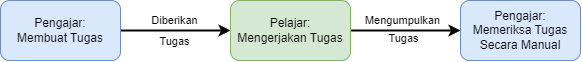
\includegraphics[width=\textwidth]{tradisional.drawio.png}
	\caption[Sistem Tradisional Pemberian Tugas]{Sistem Tradisional Pemberian Tugas}
	\label{fig:1:tradisional}
\end{figure}

\newpage

Pemberian tugas menulis kode program memiliki banyak masalah. Oleh karena itu, dibutuhkannya sistem baru untuk memberikan tugas kepada pelajar bidang informatika. Sistem baru yang dimaksud tentunya untuk melakukan penilaian secara otomatis. Sebuah sistem yang mengambil kode program pelajar dan memberikan sebuah nilai numerik yang menandakan hasil dari kode program tersebut\footnote{Kurnia, A., Lim, A., dan Cheang, B. (2001) Online judge. {\em Computers \& Education}.}. Suatu hal yang menarik, Tugas kode program dapat dibagi menjadi 2 jenis yaitu tugas individu dan tugas kelompok. Pada tugas kelompok merupakan tugas yang ditanggung oleh banyak pelajar, biasanya program yang dibuat memiliki antarmuka dan harus diperiksa oleh pengguna khusus yang mengetahui fitur-fitur yang dibutuhkan. Sedangkan tugas individu merupakan sebuah tugas yang diberikan untuk satu individu, biasanya program yang dibuat bersifat algoritmik dan tidak memerlukan antarmuka untuk dijalankan. Program algoritmik adalah sebuah jenis program yang dibuat berdasarkan algoritma untuk menyelesaikan masalah tertentu. Algoritma sendiri adalah langkah-langkah dalam pemecahan masalah secara sistematis\footnote{IDCloudHost (2020) Algoritma pemrograman beserta contohnya.
	\newblock \url{https://idcloudhost.com/blog/algoritma-pemrograman-pengertian-fungsi-cara-kerja-dan-contohnya/}.
	6 Desember 2024.}.
% FIXME: ini kalimat line 16, asa kurang tp buat memperjelas gt 
Algoritma itu seperti resep makanan, dimana akan ada bahan-bahan yang dibutuhkan dan serangkaian langkah untuk membuat suatu makanan yang dijelaskan.

Sebagian besar program yang bersifat algoritmik hanyak perlu mengambil \textit{input} dari \textit{input} standar seperti angka, huruf, dan sebuah kata atau kalimat dengan format yang sudah ditentukan, seolah-olah \textit{input} ini merupakan \textit{output} dari program lain. Kemudian program algoritmik akan memproses \textit{input} tersebut dalam komputer dan mengeluarkan hasil komputasinya dalam format yang sudah ditentukan untuk dibaca oleh program lain dan memanfaatkan hasil komputasi tersebut. Singkatnya, program algoritmik itu seperti \textit{filter} antar program. Dengan ini, sistem penilaian secara otomatis dapat dibuat dengan membuat sebuah program yang mengambil kode program, memasukkan \textit{input} sesuai format ke dalam program tersebut, membaca hasil keluaran program, dan menilai hasil keluaran program tersebut\footnote{Kurnia, A., Lim, A., dan Cheang, B. (2001) Online judge. {\em Computers \& Education}.}. Sistem penilaian otomatis \mbox{ini diberikan nama \textit{Online Judge}}. Terlebih lagi sistem ini dapat dilakukan secara \textit{offline} maupun \textit{online}. Gambar \ref{fig:1:onlinejudge} menunjukkan bagaimana \textit{online judge} berintegrasi dengan sistem \mbox{pemberian tugas yang sudah ada.}

Tugas pemrograman sudah menjadi keseharian dalam pembelajaran pada bidang informatika.
Termasuk pada perguruan tinggi pada bidang informatika, maka \textit{online judge} menjadi sebuah kebutuhan termasuk pada Universitas Katolik Parahyangan atau yang biasa disebut UNPAR.
\textit{Online Judge} yang digunakan oleh UNPAR dinamakan SharIF-Judge\footnote{Vallian, S. (2018) {Kustomisasi Sharif Judge Untuk Kebutuhan Program Studi Teknik Informatika}. Skripsi. Universitas Katolik Parahyangan, Indonesia.} yang merupakan hasil dimodifikasi oleh Stillmen Vallian terhadap Sharif-Judge\footnote{Version 1.4 (2014) {\em Sharif Judge Documentation}. Mohammad Javad Naderi. Tehran, Iran.} buatan Mohammad Javad Naderi yang dibuat menggunakan \textit{framework} CodeIgniter dan Bash. Gambar~\ref{fig:1:dashboardpng} merupakan halaman utama setelah masuk ke dalam SharIF-Judge.

\vspace{0.5cm}

\begin{figure}[H]
	\centering
	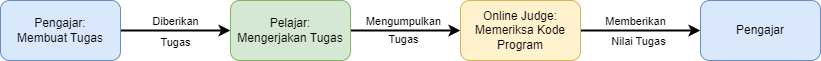
\includegraphics[width=\textwidth]{online_judge.drawio.png}
	\caption[Sistem Integrasi oleh \textit{Online Judge}]{Sistem Integrasi oleh \textit{Online Judge}}
	\label{fig:1:onlinejudge}
\end{figure}

\begin{figure}[H]
	\centering
	\includegraphics[width=\textwidth]{dashboard.png}
	\caption[Tampilan Awal SharIF Judge]{Tampilan Awal SharIF Judge}
	\label{fig:1:dashboardpng}
\end{figure}

\vspace{-0.25cm}

Ujian juga merupakan sebuah bentuk penilaian dari pengajar kepada pelajarnya. Tentunya pelajar maupun mahasiswa ingin memperoleh nilai yang memuaskan dalam ujiannya. Banyak cara yang dilakukan oleh pelajar maupun mahasiswa untuk memperoleh nilai tersebut, salah satunya adalah dengan melakukan kecurangan yaitu \textit{copy paste} atau menyalin jawaban teman atau rekan mereka\footnote{Prihatini, F.~N. dan Indudewi, D. (2016) {Kesadaran dan Perilaku Plagiarisme dikalangan Mahasiswa(Studi pada Mahasiswa Fakultas Ekonomi Jurusan Akuntansi Universitas Semarang)}. {\em Dinamika Sosial Budaya}.}. Praktek ini diperparah jika ujian dilakukan secara \textit{online}, dikarenakan pelajar dapat mengakses berbagai fasilitas di internet. Oleh karena itu, diperlukannya sebuah sistem pada sistem \textit{online judge} untuk mengawasi saat terjadinya ujian online.

Pada saat siswa mengerjakan tugas maupun ujian pembuatan kode program, umumnya pengerjaan kode tersebut dilakukan pada aplikasi eksternal seperti \textit{visual studio code} atau \textit{notepad}. Hal ini juga terjadi pada sistem dalam UNPAR dimana mahasiswa akan membuat kode program pada aplikasi eksternal. Ini membuat pengawasan saat pembuatan kode program lebih sulit untuk dilakukan, terlebih jika ujian dilakukan secara \textit{online}. Maka dari itu, Nicholas Aditya Halim memodifikasi SharIF Judge agar semua sistem pemberian tugas seperti pada gambar \ref{fig:1:onlinejudge} dapat dilakukan dalam sistem yang sama yaitu pada SharIF Judge. Sistem yang bangun oleh Nicholas Aditya Halim adalah ``Implementasi editor kode pada Sharif Judge''\footnote{Halim, N.~A. (2021) {Implementasi Editor Kode pada SharIF Judge}. Skripsi. Universitas Katolik Parahyangan,  Indonesia.}, dimana SharIF Judge ditambahkan sebuah \textit{Integrated Development Environment} atau yang disebut dengan IDE. IDE merupakan sebuah sistem yang memiliki kemampuan untuk membuat kode dalam editor kode dan menjalankan kode program tersebut. Dengan adanya IDE, seluruh proses pembuatan kode program dapat dilakukan dalam SharIF Judge. Maka dari itu, seluruh proses sistem pemberian tugas dapat dilakukan dalam satu sistem saja, yaitu SharIF Judge.

Walaupun begitu, pada dasarnya IDE yang digunakan pada SharIF Judge tidak dapat mengawasi proses pembuatan kode program dan jika terjadinya praktek \textit{copy paste} pada saat pembuatan kode program tersebut. Maka dari itu pada Tugas akhir ini, IDE pada SharIF Judge akan dimodifikasi untuk menangani hal tersebut dengan ditambahkannya fitur untuk merekam semua ketikan atau kejadian dalam editor kode dalam IDE. Lalu ketikan atau kejadian dalam editor dapat di putar kembali seperti rekaman. Fitur ini akan membuat pengawasan terhadap kegiatan kuliah lebih mudah untuk pengawas dan dapat \mbox{menjadi bukti kecurangan jika dibutuhkan.}

\newpage

\section{Rumusan Masalah}

Rumusan Masalah yang akan dibahas pada tugas akhir ini adalah:
\begin{enumerate}
	% \item Bagaimana agar editor kode lebih mudah untuk dipakai oleh mahasiswa.
	\item Bagaimana mengimplementasikan perekaman dan pemutaran ulang ketikan mahasiswa pada IDE SharIF-Judge?
	\item Bagaimana cara menyimpan data pemutaran ulang mahasiswa secara rutin dengan otomatis dan tidak mengambil penyimpanan \textit{database} sangat besar?
	\item Bagaimana tanggapan pengguna terhadap implementasi perekaman dan pemutaran ulang kode ketikan pada SharIF Judge?
\end{enumerate}

\section{Tujuan}

Tujuan yang ingin dicapai skripsi ini adalah sebagai berikut:
\begin{enumerate}
	\item Mengimplementasikan perekaman dan pemutaran ulang ketikan mahasiswa pada IDE SharIF-Judge.
	\item Mencari cara penyimpanan data efektif dan mengimplementasikannya pada perekaman dan pemutaran ulang ketikan.
	\item Mendapatkan umpan balik dari tanggapan pengguna terhadap perekaman dan pemutaran ulang ketikan mahasiswa pada SharIF-Judge.
\end{enumerate}

\section{Detail Perkembangan Pengerjaan Skripsi}
Detail bagian pekerjaan tugas akhir sesuai dengan rencan kerja/laporan perkembangan terkahir :
\begin{enumerate}
	\item \textbf{Melakukan studi mengenai bahasa pemrograman PHP\footnote{Dokumentasi php. https://www.php.net/manual/en/(10 Desember 2024)}.}\\
	      {\bf Status :} Ada sejak rencana kerja skripsi.\\
	      {\bf Hasil :} Bahasa pemrograman PHP sudah dipelajari.

	      Berikut merupakan ringkasan dari hasil pembelajaran bahasa pemrograman PHP.

	      PHP atau \textit{Hypertext Preprocessor} merupakan sebuah \textit{scripting language} yang dibuat untuk web development\footnote{https://www.php.net/}. Awalnya PHP dibuat oleh Denmark-Kanada dan Rasmus Lerdorf pada tahun 1993 dan dirilis pada tahun 1995.

	      Untuk membuat \textit{file} php, \textit{file} akan memiliki extensi \verb|php| seperti contohnya adalah \verb|index.php|. Biasanya \textit{file} PHP akan di proses pada web servernya oleh sebuah PHP \textit{interpreter}. Pada \textit{file} php, tag \verb|<?php| menandakan dimana php \textit{interpreter} akan menterjemahkan teks menjadi kode php, sedangkan diluar tag tersebut akan dianggap sebagai HTML biasa. Dalam PHP, \verb|echo| menandakan dimana PHP interpreter akan mencetak text dimana kutik ke dalam HTML. Berikut contoh kode \ref{kode:5:simplephp} sederhana dari \textit{file} php.

	      \begin{lstlisting}[language={php}, caption={Contoh Sederhana \textit{File} PHP}, label={kode:5:simplephp}]
Hello 
<? php
echo 'World'
?>
		  \end{lstlisting}

	      Kode \ref{kode:5:simplephp} akan menghasilkan tulisan \verb|Hello World| pada websitenya. Sebagai umum bahasa pemrograman, PHP memiliki beberapa fitur yang umum yaitu sebagai berikut:

	      \begin{itemize}
		      \item \textbf{Comments} \\
		            Salah satu hal yang penting dalam bahasa pemrograman adalah untuk memberikan komentar di dalam kodenya. Ada beberapa cara untuk memberikan komentar yaitu sebagai berikut:

		            \begin{lstlisting}[language={php}, caption={Contoh Komentar Satu baris}, label={kode:5:commentoneline}]
// komentar satu baris
/* komentar sebagian kode dalam suatu baris */
			  		\end{lstlisting}

		            Untuk memberikan komentar untuk beberapa baris, caranya adalah sebagai berikut:

		            \begin{lstlisting}[language={php}, caption={Contoh Komentar Banyak Baris}, label={kode:5:commentmanyline}]
/*
Ini
Sebuah
Komentar
*/

// atau 

/* Ini
 * Juga
 * Sebuah
 * Komentar
 */
			  \end{lstlisting}

		      \item \textbf{Variabel} \\ % ada jg print var_dump
		            Pada PHP, untuk mendefinisikan sebuah variabel dimulai dengan tanda \verb|$|, dan diikuti oleh sekumpulan karakter alfabet, nomor, dan simbol \verb|_|. Nama variabel pada PHP juga \textit{case-sensitive}, yang berarti nama \verb|$text| dan \verb|$Text| merupakan variabel yang berbeda.
		            PHP juga tidak perlu dan tidak bisa mendeklarasi variabel. Setelah variabel diberikan nilai, PHP akan membuat variabel dengan tipe sesuai dengan nilai yang diberikan. Seperti contoh untuk membuat variabel adalah sebagai berikut:

		            \begin{lstlisting}[language={php}, caption={Contoh Pembuatan Variabel}, label={kode:5:variabel_ex}]
$isPerson = TRUE
$name = 'Kenzhi'
$age = 20
					\end{lstlisting}

		            PHP juga tidak akan mengeluarkan error ketika variabel dengan tipe angka di tetapkan kembali nilainya seperti \verb|$age = 'remaja'|.

		            Jika ingin mengetahui isi nilai variabel, dapat menggunakan fungsi \verb|var_dump()|. Sebagai contoh untuk mengetahui variabel \verb|$name| akan dipanggil \verb|var_dump($name)|.

		      \item \textbf{Type} \\
		            Bahasa pemrograman juga memiliki tipe-tipe variabel. Tipe-tipe dalam PHP adalah sebagai berikut:

		            \begin{itemize}
			            \item \verb|bool|: nilai boolean (\verb|TRUE| atau \verb|FALSE|)
			            \item \verb|int|: bilangan bulat
			            \item \verb|float|: bilangan ril
			            \item \verb|string|: sebuah teks atau string
			            \item \verb|array|: sebuah array
			            \item \verb|object|: sebuah object
			            \item \verb|null|: nilai yang menandakan nilai yang tidak diberikan
		            \end{itemize}

		      \item \textbf{Operators} \\
		            Dalam PHP juga memiliki operators seperti umumnya. Pengunaan operator dalam PHP itu mengikuti bahasa pemrograman umum, contoh pengguna operator adalah sebegai berikut:

		            \begin{center}
			            \verb|{nilai} {operator} {nilai}|
		            \end{center}

		            Dalam bahasa pemrograman PHP, Operator dapat dibagi menjadi 5 bagian yaitu:

		            \begin{itemize}
			            \item \textbf{Assignment Operators} \\
			                  \textit{Assigment Operator} digunakan untuk memberikan nilai kepada variabel. Hanya ada satu \textit{assignment operator} pada PHP yaitu \verb|=|. Pengunaan \textit{assignment operator} berbeda dengan lainnya dikarenakan nilai pertamanya menjadi sebuah \textit{variabel}. Sebagai contoh cara menggunakan \textit{assignment operator} adalah sebagai berikut:

			                  \begin{center}
				                  \verb|$variabel = 'isi variabel'|
			                  \end{center}

			            \item \textbf{Arithmetic Operators} \\
			                  \textit{Arithmetic Operators} digunakan untuk melakukan operasi matematika dasar, seperti penjumlahan, pengurangan, perkalian, dan sebagainya. Pada PHP, ada beberapa \textit{arithmetic operators} yaitu sebagai berikut:

			                  \begin{itemize}
				                  \item \verb|+| : Penjumlahan
				                  \item \verb|-| : Pengurangan
				                  \item \verb|*| : Perkalian
				                  \item \verb|/| : Pembagian
				                  \item \verb|%| : Sisa bagi (modulo)
				                  \item \verb|**| : Perpangkatan
			                  \end{itemize}

			            \item \textbf{Comparasion Operators} \\
			                  \textit{Comparasion Operators} digunakan untuk melakukan perbandingan antara dua nilai yang akan menghasilkan sebuah nilai boolean. Pada PHP, ada beberapa \textit{comparasion operator} yaitu sebagai berikut:

			                  \begin{itemize}
				                  \item \verb|<| : Lebih kecil dari
				                  \item \verb|<=| : Lebih kecil atau sama dengan
				                  \item \verb|>| : Lebih besar dari
				                  \item \verb|>=| : Lebih besar atau sama dengan
				                  \item \verb|==| : Sama dengan (mencek isi nilai sama. `\verb|==|' akan tetap mengamggap nilai sama walaupun memiliki tipe yang berbeda. Seperti contoh \verb|1 == '1'| akan mengembalikan \verb|TRUE|)
				                  \item \verb|===| : Sama dengan (mencek isi nilai dan tipe nilai yang sesuai. Seperti contoh \verb|1 === '1'| akan mengembalikan \verb|FALSE|)
				                  \item \verb|!=| : tidak sama dengan (mencek isi nilai, kebalikan dari `\verb|==|')
				                  \item \verb|!==| : tidak sama dengan (menccek isi nilai dan juga tipe nilai, kebalikan dari `\verb|===|')
			                  \end{itemize}

			            \item \textbf{Logical Operators} \\
			                  \textit{Logical Operators} digunakan untuk melakukan operasi logika dengan dua atau lebih nilai boolean. Hasil dari \textit{logical operators} adalah sebuah nilai boolean. Pada PHP, ada beberapa \textit{logical operators} yaitu sebagai berikut:

			                  \begin{itemize}
				                  \item \verb|&&| atau \verb|and| : menghasilkan \verb|TRUE| jika kedua nilai bernilai \verb|TRUE|
				                  \item \verb|||| atau \verb|or| : menghasilkan \verb|TRUE| jika salah satu nilai bernilai \verb|TRUE|
				                  \item \verb|xor| : menghasilkan \verb|TRUE| jika kedua nilai berbeda.
			                  \end{itemize}

			            \item \textbf{Unary Operators} \\
			                  \textit{Unary Operators} adalah operator yang bekerja dengan hanya satu operand. Operator ini sering digunakan untuk memodifikasi atau mengoperasikan nilai dari satu variabel saja. Pada PHP hanya ada dua \textit{unary oprator} yaitu:

			                  \begin{itemize}
				                  \item \verb|++| : Meningkatkan nilai variabel sebesar satu (Penggunaan didepan nilai)
				                  \item \verb|--| : Mengurangi nilai variabel sebesar satu (Penggunaan didepan nilai)
				                  \item \verb|!| : Negasi sebuah nilai boolean (Penggunaan dibelakang nilai)
			                  \end{itemize}
		            \end{itemize}

		      \item \textbf{Strings} \\
		            Dalam PHP, String merupakan sebuah tipe. Untuk mendeklarasi sebuah string dalam variabel dapat menggunakan kutip tunggal (\verb|'|) atau kutip ganda (\verb|"|). Perbedaan kedua kutip adalah dengan tanda kutip ganda string dapat dimasukkan oleh variabel lain dan juga dapat dimasukkan \textit{escape characters} seperti \textit{new line} (\verb|\n|) atau tabs (\verb|\t|). Seperti contohnya adalah

		            \begin{lstlisting}[language={php}, caption={Contoh Pembuatan String}, label={kode:5:string_ex}]
$test = 'an example';

$example = "This is $test"; // Keluaran: 'This is an example'
					\end{lstlisting}

		            Variabel string juga dapat di concat atau digabungkan dengan menggunakan simbol titik (\verb|.|). Contohnya adalah sebagai berikut:

		            \begin{lstlisting}[language={php}, caption={Contoh Penggabungan String}, label={kode:5:stringconcat}]
$firstName = 'Andreas';
$lastName = 'Ronaldi';

$fullName = $firstName . ' ' . $lastName; // Keluaran: 'Andreas Ronaldi'
					\end{lstlisting}

		            \begin{comment}
		            Ada beberapa fungsi pada string yang seding digunakan. Kode \ref{kode:5:stringmethod} menunjukkan fungsi-fungsi untuk tipe string.

		            \begin{lstlisting}[language={php}, caption={Fungsi Untuk Tipe String}, label={kode:5:stringmethod}]
$teks = 'string'
// Mengeluarkan panjang variabel string, jika tidak ada
strlen($teks) // Keluaran: 6.

// Mengambil sebagian teks dari variabel 
substr($teks, 3) // Keluaran: 'ing'. Mengambil dari index 3 hingga akhir
substr($teks, 3, 2) // Keluaran: 'in'. Di mulai index 3, ambil 2 huruf saja

// Mengubah sebagian teks menjadi teks lain
str_replace('ring', 'ep', $teks) // Keluaran: 'step'. Mengubah 'ring' menjadi 'ep'

// Fungsi-fungsi lain yang berguna adalah:
// trim() : menghilangkan spasi di awal dan akhir teks
// strtoupper() : membuat string menjadi huruf besar
// strtolower() : membuat string menjadi huruf kecil
// ucfirst() : membuat karakter pertama menjadi huruf besar
// strpos() : menemukan kemunculan pertama sebuah teks dalam string
// explode() : membagi string menjadi sebuah array
// implode() : menggabungkan array menjadi sebuah string
					\end{lstlisting}
		            \end{comment}

		      \item \textbf{Array} \\
		            Array merupakan sebuah tipe variabel dalam PHP. Array merupakan daftar nilai yang dikelompokkan di bawah satu nama umum. Dalam PHP, isi dalam array tidak harus memiliki tipe yang sama. Untuk mendeklarasi sebuah variabel array dapat menggunakan tanda kurung kotak \verb|[]|. Contoh deklarasi array adalah sebagai berikut:

		            \begin{lstlisting}[language={php}, caption={Contoh mendeklarasi variabel array}, label={kode:5:array_ex}]
// Mendeklarasi array kosong
$array = [];
$array = array();

// Mendeklarasi array dengan isi
$array = [1, 'str'];
$array = array(1, 'str');
			  		\end{lstlisting}

		            Seperti bahasa pemrograman lainnya untuk mengakses sebuah nilai dalam array, dapat menggunakan \textit{index} yang dimulai dengan angka 0. Seperti contoh \verb|$arr| memiliki tiga nilai yaitu \verb|['a', 'b',| \verb|'c']|. Dapat dilihat nilai \verb|'b'| ada pada nilai ke dua. Dikarenakan index dimulai dari angka 0, maka untuk mengakses \verb|'b'|, Maka untuk mengakses \verb|'b'| butuh mengakses index ke satu dengan menggunakan kurung kotak (\verb|[]|) setelah nama variabel array, Jadi hasil notasi \mbox{untuk~mengakses}~\verb|'b'|~adalah~\verb|$arr[1]|.

		            \begin{comment}
		            Ada beberapa fungsi yang sering digunakan untuk variabel array yaitu sebagai berikut:

		            \begin{itemize}
			            \item \verb|array_unshift()| : Menambahkan nilai ke awal array
			            \item \verb|count()| : Menghitung banyak nilai dalam array
			            \item \verb|in_array()| : Mencek jika array memiliki nilai tertentu
			            \item \verb|is_array()| : Memeriksa apakah sebuah variabel adalah array
			            \item \verb|array_unique()| : Menghapus nilai duplikat dari array
			            \item \verb|array_search()| : Mencari nilai dalam array dan mengembalikan indexnya
			            \item \verb|array_reverse()| : Membalikkan array
			            \item \verb|array_reduce()| : Mengurangi array menjadi satu nilai
			            \item \verb|array_map()| : Menerapkan sebuah fungsi ke setiap item dalam array.
			            \item \verb|array_filter()| : Memfilter array menggunakan sebuah fungsi.
			            \item \verb|max()| : Mendapatkan nilai maksimum dalam array.
			            \item \verb|min()| : Mendapatkan nilai minimum dalam array.
			            \item \verb|array_rand()| : Mendapatkan nilai acak dari array.
			            \item \verb|array_count_values()| : Menghitung semua nilai yang ada di dalam array.
			            \item \verb|implode()| : Mengubah array menjadi sebuah string.
			            \item \verb|array_pop()| : Menghapus nilai terakhir dari array dan mengembalikan nilainya.
			            \item \verb|array_shift()| : seperti \verb|array_pop()| tetapi menghapus nilai pertama, bukan yang terakhir.
			            \item \verb|sort()| : Mengurutkan array.
			            \item \verb|rsort()| : Mengurutkan array dalam urutan terbalik.
			            \item \verb|array_walk()| : seperti \verb|array_map()| melakukan sesuatu untuk setiap item dalam array, tetapi sebagai tambahan, \verb|array_walk()| dapat mengubah nilai dalam array yang ada
		            \end{itemize}
		            \end{comment}

		      \item \textbf{Associative Arrays} \\ % array key string
		            Dalam array biasa, index merupakan sebuah angka yang terus bertambah yang dimulai dari 0. Tetapi \textit{associative array} menggunakan index yang berbeda-beda seperti menggunakan string atau teks. Index pada \textit{associative array} dinamakan \textit{key}. Berikut contoh mendeklarasi sebuah \textit{associative~array}:

		            \begin{lstlisting}[language={php}, caption={Contoh mendeklarasi associative array}, label={kode:5:aarrayex}]
$list = ['first' => 'a', 'second' => 'b'];

$list['first'] // Keluaran: 'a'
$list['second'] // Keluaran: 'b'
					\end{lstlisting}

		            \begin{comment}
		            Ada beberapa fungsi yang sering digunakan untuk variabel \textit{associative array} yaitu sebagai berikut:

		            \begin{itemize}
			            \item \verb|array_key_exists()| : Memeriksa apakah sebuah \textit{key} ada dalam array.
			            \item \verb|array_keys()| : Mendapatkan semua \textit{key} dari array.
			            \item \verb|array_values()| : Mendapatkan semua nilai dari array.
			            \item \verb|asort()| : Mengurutkan \textit{associative array} berdasarkan nilai.
			            \item \verb|arsort()| : Mengurutkan \textit{associative array} dalam urutan menurun berdasarkan nilai.
			            \item \verb|ksort()| : Mengurutkan \textit{associative array} berdasarkan \textit{key}.
			            \item \verb|krsort()| : Mengurutkan \textit{associative array} dalam urutan menurun berdasarkan \textit{key}.
		            \end{itemize}
		            \end{comment}

		      \item \textbf{Conditionals} \\ % if else
		            Dalam PHP, \textit{conditional} digunakan untuk mengeksekusi blok kode tertentu berdasarkan suatu kondisi, biasanya kondisi ini merupakan sebuah boolean. \textit{Conditional} membantu mengontrol jalan kode program dengan memungkinkan tindakan yang berbeda untuk diambil tergantung pada kondisi yang diberikan. Berikut notasi pengguna \textit{conditional} dalam PHP:

		            \begin{lstlisting}[language={php}, caption={Notasi conditional}, label={kode:5:con_notasi}]
if ($condition) {
	// kode blok akan dijalankan saat $condition merupakan TRUE
} elseif ($condition2) {
	// jika kondisi di atas kondisi elseif ini merupakan FALSE, maka kode blok dapat dijalankan saat $condition2 merupakan TRUE.
	// elseif dapat di buat sebanyak yang diinginkan.
} else {
	// jika semua kondisi di atas merupakan FALSE, maka kode blok akan dijalankan.
}
			  		\end{lstlisting}

		            Kode \ref{kode:5:con_notasi} menunjukkan berbagai notasi \textit{conditional} yaitu \verb|if|, \verb|elseif|, dan \verb|else|.
		            Pernyataan \verb|if| digunakan untuk menjalankan sebuah blok kode jika kondisi tertentu bernilai benar.
		            Pernyataan \verb|elseif| (atau else if) berfungsi untuk mencek beberapa kondisi. Jika kondisi dalam \verb|if| salah, PHP akan beralih ke blok \verb|elseif| untuk memeriksa apakah kondisi tersebut benar. Jika benar, kode di dalam blok tersebut akan dijalankan. Jika kondisi tersebut juga salah, program akan beralih ke blok \verb|elseif| berikutnya atau blok else jika ada.
		            Jika salah satu kondisi sudah dipenuhi, maka semua kondisi berikutnya tidak ada dijalankan.
		            Kode \ref{kode:5:con_ex} merupakan contoh penggunaan conditional dalam bahasa pemrograman PHP.

		            \begin{lstlisting}[language={php}, caption={Contoh Penggunaan Conditional}, label={kode:5:con_ex}]
$time = 14;

if ($time < 12) {
	echo "Good morning!"; // karena $time lebih besar dari 12, maka kondisi pertama gagal.
} elseif ($time < 18) {
	echo "Good afternoon!"; // kode akan dijalankan karena $time masih lebih kecil dari 18.
} else {
	echo "Good evening!"; // kode tidak dijalankan karena kondisi di atas sudah ada yang memenuhi.
}

// Keluaran: Good afternoon!
			  		\end{lstlisting}

		            Seperti bahasa programming yang umum digunakan juga, PHP memiliki notasi \verb|switch|. \textit{Switch} digunakan ketika Anda memiliki banyak kondisi berdasarkan variabel tunggal. Umumnya \textit{switch} lebih mudah dibaca ketika beberapa kondisi if/elseif yang memeriksa variabel yang sama.
		            Berikut merupkan notasi penggunaan \verb|switch|:

		            \begin{lstlisting}[language={php}, caption={Notasi switch}, label={kode:5:switch_notasi}]
switch (variabel) {
	case nilai1:
		// kode blok yang akan dijalankan hingga ditemukan break jika variabel sama dengan nilai1
		break;
	default:
		// kode blok yang akan dijalankan jika tidak ada kasus yang sesuai
}
					\end{lstlisting}

		            \begin{lstlisting}[language={php}, caption={Contoh Penggunaan switch}, label={kode:5:switch_ex}]
$day = 3;

switch ($day) {
	case 1:
		echo "Monday";
		break;
	case 2:
		echo "Tuesday";
		break;
	case 3:
		echo "Wednesday";
		break;
	default:
		echo "Invalid day";
}

// Keluaran: Wednesday 
					\end{lstlisting}

		            Kode \ref{kode:5:switch_ex} merupakan contoh penggunaan \verb|switch| dalam PHP.

		      \item \textbf{Loops} \\
		            Dalam PHP, loop digunakan untuk menjalankan blok kode secara berulang-ulang selama kondisi yang ditentukan benar. Perulangan membantu mengotomatiskan tugas-tugas yang berulang dan mengurangi kebutuhan untuk menulis kode yang sama beberapa kali. PHP memiliki beberapa jenis perulangan yaitu \verb|while|, \verb|do-while|, \verb|for|, dan \verb|foreach|. Berikut penjelasan untuk setiap jenis perulangan dalam PHP:

		            \begin{itemize}
			            \item \verb|while| \\
			                  \verb|While| adalah perulangan yang paling sederhana. \verb|While| akan terus mengulang jika kondisi tertentu itu benar. Notasi penggunaan \verb|while| adalah sebagai berikut:

			                  \begin{lstlisting}[language={php}, caption={Notasi while}, label={kode:5:while_notasi}]
while ($condition) {
	// kode blok yang berulang.
}
							  \end{lstlisting}

			            \item \verb|do-while| \\
			                  \verb|do-while| mirip dengan \verb|while|, perbedaannya adalah \verb|do-while| akan memeriksa kondisi setelah menjalankan blok kode. Hal tersebut membuat blok kode akan selalu dijalankan setidaknya sekali, meskipun kondisi awalnya salah.

			                  \begin{lstlisting}[language={php}, caption={Notasi do-while}, label={kode:5:do-while_notasi}]
do {
	// kode blok yang berulang.
} while ($condition);
								\end{lstlisting}

			            \item \verb|for| \\
			                  \verb|For| mirip dengan \verb|while|, tetapi untuk mendefinisikan variabel yang digunakan dalam kondisi sebelum perulangan, dan untuk menaikkan variabel kondisi tersebut secara manual, semuanya dilakukan pada baris dalam \verb|for|. Kode \ref{kode:5:for_notasi} merupakan notasi untuk menggunakan~\verb|for|~dalam~PHP.

			                  \begin{lstlisting}[language={php}, caption={Notasi for}, label={kode:5:for_notasi}]
for (initialization; condition; increment/decrement) {
	// kode blok yang berulang.
}
								\end{lstlisting}

			                  \begin{lstlisting}[language={php}, caption={Contoh Penggunaan for}, label={kode:5:for_ex}]
for ($i = 0; $i < 10; $i++) {
  echo $i;
}
								\end{lstlisting}

			                  Kode \ref{kode:5:for_ex} merupakan contoh penggunaan \verb|for|. Dimana \verb|$i| langsung dideklarasikan dalam baris \verb|for|, dan penambahan pada variabel \verb|$i| juga ada pada baris yang sama.

			            \item \verb|foreach| \\
			                  \verb|Foreach| secara khusus digunakan untuk mengulang nilai dalam sebuah array. \verb|Foreach| ini ideal untuk mengulang semua nilai dalam array (baik array biasa maupun associative array) tanpa perlu mengelola indeks atau penghitung secara manual. Untuk notasi penggunaan \verb|foreach| adalah sebagai berikut:

			                  \begin{lstlisting}[language={php}, caption={Notasi foreach}, label={kode:5:foreach_notasi}]
// untuk mendapatkan nilai dalam array maupun associative array
foreach ($array as $value) {
	// Kode yang akan dijalankan (dapat mengakses variabel $value)
}

// untuk mendapatkan nilai beserta key dalam array maupun associative array
foreach ($array as $key => $value) {
    // Kode yang akan dijalankan (dapat mengakses variabel $key dan $value)
}
						\end{lstlisting}

		            \end{itemize}

		      \item \textbf{Functions} \\
		            Pada bahasa pemrograman PHP, \textit{function} atau fungsi adalah sebuah blok kode yang dapat digunakan kembali yang dibuat untuk melakukan sebuah tugas tertentu. Fungsi digunakan untuk membantu menyusun kode agar lebih terstruktur dan mengurangi pengulangan kode yang sama.

		            \begin{lstlisting}[language={php}, caption={Notasi fungsi}, label={kode:5:fungsi_notasi}]
function functionName($parameter1, $parameter2, ...) {
    // Code to be executed
	return $nilai; // Mengembalikan nilai ke pemanggil fungsi
}
			  \end{lstlisting}

		            Kode \ref{kode:5:fungsi_notasi} merupakan notasi untuk membuat fungsi dalam PHP. Dimulai dengan \textit{keyword function}, dilanjutkan dengan nama fungsinya, selanjutnya terdapat kurung `()' yang didalamnya dapat diberikan parameter, dan terakhir diikuti oleh kurung kurawal `{}'. Parameter dalam fungsi itu bersifat opsional, dan digunakan untuk menerima variable dari luar kedalam fungsi tersebut. Tetapi saat fungsi dipanggil jika memiliki parameter maka pemberian paramater untuk fungsi itu bersifat wajib, jika tidak memiliki parameter yang tepat maka php \textit{interpreter} akan mengeluarkan error. Pada kode \ref{kode:5:fungsi_notasi} dalam blok kode, ada sebuah \textit{keyword} \verb|return| yang berarti fungsi akan mengembalikan nilai \verb|$nilai| (yang dapat diganti menjadi apapun) ke pemanggil fungsi tersebut.

		            Untuk memanggil sebuah fungsi dalam PHP dapat menggunakan notasi seperti berikut.

		            \begin{center}
			            \verb|functionName($parameter1, $parameter2, ...)|
		            \end{center}

		            Dalam fungsi jika parameter dapat memiliki nilai awal, jadi jika saat pemanggil fungsi tidak memiliki parameternya tidak akan terjadi error. Contoh penggunaan fungsi dengan nilai awal adalah sebagai berikut:

		            \begin{lstlisting}[language={php}, caption={Contoh Penggunaan fungsi}, label={kode:5:fungsi_ex}]
function sapa($name = "Tamu") {
    echo "Hello, $name!";
}

sapa("Alice");  // Keluaran: Hello, Alice!
sapa();         // Keluaran: Hello, Tamu!
					\end{lstlisting}

		            Dalam PHP, fungsi tidak dapat mengakses variabel yang terdapat di luar fungsinya itu sendiri kecuali dalam blok kode fungsi ditambahkan deklarasi \textit{keyword} \verb|global|. Seperti contohnya untuk mengakses variabel \verb|$varGlobal| maka harus ditambahkan \verb|global $varGlobal| sebelum mengakses variabel tersebut dalam fungsi.

		            \begin{lstlisting}[language={php}, caption={Contoh fungsi dengan variabel global}, label={kode:5:fungsi_exglobal}]
$varGlobal = "global variabel";

function myFunc() {
	global $varGlobal;
	echo $varGlobal; // Keluaran: global variabel
}

myFunc();
					\end{lstlisting}

		            PHP juga menyediakan cara untuk memanggil fungsi menggunakan nama fungsi yang disimpan dalam variabel. Seperti contohnya adalah sebagai berikut:

		            \begin{lstlisting}[language={php}, caption={Contoh pemanggil fungsi menggunakan variabel}, label={kode:5:fungsi_exname}]
function hello() {
	echo "Hello, World!";
}

$namaFungsi = "hello"; // nama fungsi yang dimasukkan kedalam kutik ganda
$namaFungsi();  // Keluaran: Hello, World!
					\end{lstlisting}

		            PHP juga memiliki \textit{anonymous function}, yaitu fungsi yang tidak memiliki nama. Fungsi ini dapat disimpan dalam variabel, diteruskan sebagai argumen, atau digunakan sebagai callback. Notasi penggunaan \textit{anonymous function} adalah sebagai berikut:

		            \begin{lstlisting}[language={php}, caption={Contoh anonymous function}, label={kode:5:fungsi_exanon}]
$myfunction = function() {
	// Kode blok yang dijalankan
};
$myfunction();
					\end{lstlisting}

		            Dalam \textit{anonymous function}, bisa digunakan \textit{keyword} \verb|use| untuk mendapatkan variable yang dideklarasikan diluar fungsi. Contoh penggunaan \verb|use| adalah sebagai berikut:


		            \begin{lstlisting}[language={php}, caption={Contoh penggunaan use}, label={kode:5:fungsi_exuse}]
$test = 'test';
$myfunction = function() use ($test) {
	echo $test;
	return 'ok';
};
$myfunction(); // Keluaran : test
					\end{lstlisting}

		            Selanjutnya adalah fungsi bernama \textit{callback} yang merupakan fungsi yang diteruskan sebagai parameter ke dalam fungsi lain. \textit{Callback} sering digunakan dalam {event handling} atau manipulasi variable array. Contoh penggunaan \textit{callback} adalah sebagai berikut:

		            \begin{lstlisting}[language={php}, caption={Contoh penggunaan callback}, label={kode:5:fungsi_excallback}]
function sayHello($name) {
	echo "Hello, $name!";
}

function greetUser($callback) {
	$callback("Andreas");  // Call the passed callback function
}

greetUser("sayHello");  // Keluaran: Hello, Kenzhi!
					\end{lstlisting}

		            Terakhir adalah fungsi bernama \textit{arrow function} yang merupakan sebuah \textit{anonymous function} yang hanya memiliki satu ekspresi atau satu baris saja dan langsung mengembalikan ekspresi tersebut secara langsung. Contohnya adalah sebagai berikut:

		            \begin{lstlisting}[language={php}, caption={Contoh penggunaan array function}, label={kode:5:fungsi_exarrow}]
$multiply = fn($a, $b) => $a * $b;

$multiply(2, 4) // Keluaran: 8
					\end{lstlisting}

		            Parameter dan keluaran dalam fungsi dapat di \textit{assign} sebuah tipe agar tidak terjadi error saat penjalanan kode program contohnya adalah sebagai berikut:

		            \begin{lstlisting}[language={php}, caption={Contoh penggunaan array function}, label={kode:5:fungsi_ex_type}]
// tipe dalam parameter
function sendEmail(string $to, string $subject, string $body) {
  //...
}

// tipe untuk keluaran fungsi
function sendEmail($to): bool {
    return true;
}
					\end{lstlisting}

		      \item \textbf{Class} \\
		            \textit{Class} atau kelas adalah konsep dasar dalam Pemrograman Berorientasi Objek atau OOP. Kelas adalah sebuah \textit{blueprint} untuk sebuah \textit{object}. Dalam kelas, bisa terdapat \textit{attributes} (variabel) dan \textit{methods} (fungsi) yang mendefinisikan suatu object.

		            Untuk mendeklarasi sebuah kelas dalam PHP, dibutuhkannya \textit{keyword class} diikuti dengan nama kelas tersebut dan tanda kurung kurawal yang dapat diisi oleh \textit{attributes} dan \textit{methods}. Untuk membuat sebuah \textit{attributes} atau \textit{methods} dibutuhkannya \textit{keyword visibility} yang terdiri dari \verb|public|, \verb|protected|, dan \verb|private|. \textit{visibility} \verb|public| membuat \textit{attributes} atau \textit{methods} dapat akses dimanapun. \textit{visibility} \verb|protected| hanya dapat diakses oleh kelas tersebut dan kelas yang di \textit{inherited}. \textit{visibility} \verb|private| hanya dapat diakses oleh kelas tersebut.

		            Notasi pembuatan kelas adalah sebagai berikut:

		            \begin{lstlisting}[language={php}, caption={Notasi Kelas}, label={kode:5:class_notasi}]
class ClassName {
	// Attributes
    public $variable1;
    private $variable2;

    // Methods
    public function method1() {
        // Kode untuk fungsi method1
    }

    private function method2() {
        // Kode untuk fungsi method2
    }
}
					\end{lstlisting}

		            \begin{lstlisting}[language={php}, caption={Contoh Kelas}, label={kode:5:class_ex}]
class Dog {
	public $name;
	
	public function bark() {
		echo $this->name . ' barked!';
	}
}
					\end{lstlisting}

		            Kode \ref{kode:5:class_ex} adalah contoh mendeklarasi sebuah kelas. Dimana \verb|Dog| memiliki sebuah \textit{attributes} \verb|$name| dan \textit{methods} \verb|bark()|. Pada \textit{methods} sebuah kelas untuk mengakses \textit{attributes} dan \textit{methods} lainnya dapat menggunakan \textit{keyword} \verb|$this|. \textit{methods} \verb|bark()| terdapat \verb|$this->name| yang akan mengakses \textit{attributes} \verb|$name| dalam kelas tersebut.

		            Untuk memanggil kelas, dibutuhkannya object dengan kelas tersebut.  Untuk membuat object dengan kelas tertentu dapat menggunakan \textit{keyword new} di sebelum nama kelas. Setelah itu kelas baru akan di \textit{assign} kedalam sebuah variabel. Melalui variabel itu, \textit{attributes} dan \textit{methods} kelas tersebut dapat di akses.
		            Untuk memanggil \textit{attributes} atau \textit{methods} dalam variabel tersebut, butuh sebuah tanda baca panah (\verb|->|) yang menandakan php \textit{interpreter} untuk mengakses ke dalam instance object tersebut. Untuk
		            Seperti contoh menggunakan kode \ref{kode:5:class_ex} untuk membuat kelas baru dan mengakses data didalam kelas tersebut adalah sebegai berikut:

		            \begin{lstlisting}[language={php}, caption={Contoh Pemanggilan Kelas}, label={kode:5:class_call_ex}]
$robert = new Dog();
$robert->name = 'Robert';
$robert->bark(); // Keluaran: Robert barked!
					\end{lstlisting}

		            Pada saat membuat kelas baru ke dalam sebuah variabel, setelah nama kelas ada tanda kurung `()' seperti pada pemanggil sebuah fungsi. Sebenarnya kelas memiliki method awal bernama \verb|_construct| yang digunakan untuk membangun object kelas tersebut pada saat object dibuat. Fungsi \verb|_construct| akan dipanggil dengan parameter yang ada saat object baru dibuat. Berikut perubahan yang akan pada Kode \ref{kode:5:class_ex} dan Kode \ref{kode:5:class_call_ex}:

		            \begin{lstlisting}[language={php}, caption={Contoh Kelas}, label={kode:5:class_ex}]
class Dog {
	public $name;
	
	public function __construct($name) {
        $this->name = $name;
  	}
	
	public function bark() {
		echo $this->name . ' barked!';
	}
}

$robert = new Dog('Robert');
$robert->bark(); // Keluaran: Robert barked!
					\end{lstlisting}

		            Seperti pada fungsi, \textit{attributes} dan \textit{methods} dapat ditambahkan tipe untuk mengurangi \textit{error}. Contoh perubahan yang adalah sebagai berikut:

		            \begin{lstlisting}[language={php}, caption={Contoh Kelas}, label={kode:5:class_ex}]
class Dog {
	public string $name;
	
	public function __construct(string $name) {
		$this->name = $name;
	}
	
	public function bark(): string {
		return $this->name . ' barked!';
	}
}

$robert = new Dog('Robert');
echo $robert->bark(); // Keluaran: Robert barked!
					\end{lstlisting}

		      \item \textbf{Exceptions} \\
		            Dalam PHP, \textit{Exceptions} dapat ditangani dengan menggunakan \verb|try|, \verb|catch|, dan jika dibutuhkan \verb|finally|. Notasi penggunaan \textit{exception} dalam PHP adalah sebagai berikut:

		            \begin{lstlisting}[language={php}, caption={Notasi Penggunaan Exception}, label={kode:5:exception_notasi}]
try {
    // Kode blok yang mungkin akan mengeluarkan error atau exception
} catch (Exception $e) {
    // Kode blok yang mengatasi jika terjadi the exception
} finally {
    // Kode blok yang pasti akan dijalankan setelah try/catch
}
			  \end{lstlisting}

	      \end{itemize}


	      %   https://www.freecodecamp.org/news/the-php-handbook/
	      % https://en.wikipedia.org/wiki/PHP#


	\item \textbf{Melakukan studi literatur mengenai \textit{framework} CodeIgniter 3\footnote{Dokumentasi CodeIgniter 3 https://codeigniter.com/userguide3/(10 Desember 2024)}.} \\
	      {\bf Status :} Ada sejak rencana kerja skripsi.\\
	      {\bf Hasil :} Sudah melakukan studi mengenai cara kerja \textit{framework} CodeIgniter 3.

	      Berikut ringkasan hasil studi mengenai \textit{framework} CodeIgniter 3:

	      CodeIgniter 3 adalah sebuah \textit{framework opensource} untuk mempermudah pengguna dalam membangun sebuah aplikasi \textit{website} menggunakan bahasa PHP. CodeIgniter 3 bertujuan untuk membantu pengguna dalam membangun sebuah aplikasi \textit{website} lebih cepat dengan menyedikan \textit{library} yang beragam dengan fungsi yang umum digunakan dan tampilan dan \textit{logic} yang simpel. Gambar \ref{fig:2:ciflowchart} merupakan bagaimana data mengalir pada sistem CodeIgniter.

	      \begin{figure}[H]
		      \centering
		      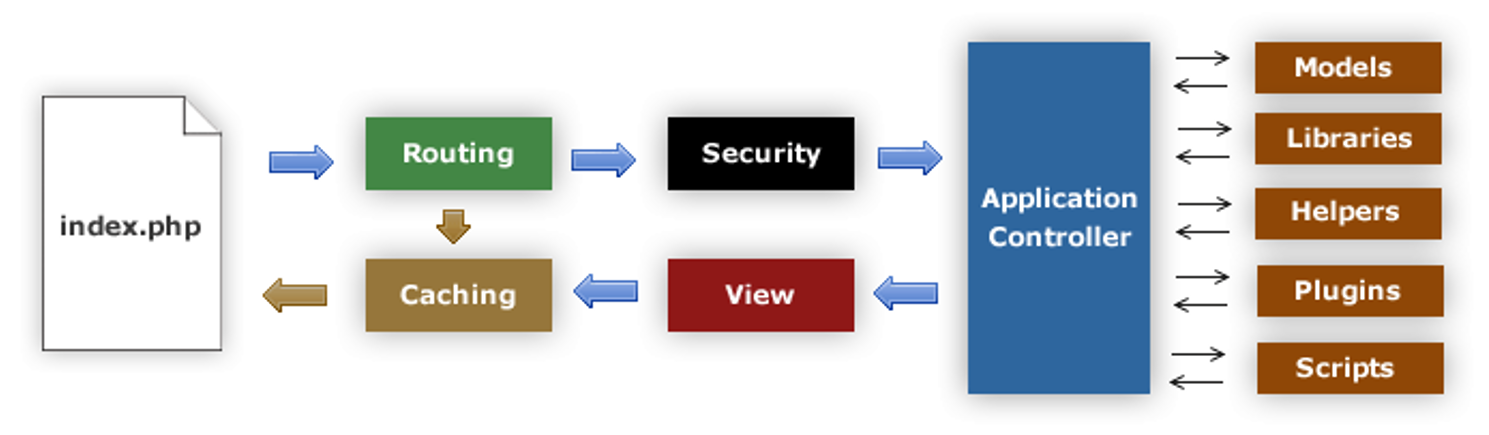
\includegraphics[scale=0.275]{ci-flowchart.png}
		      \caption{\textit{Flow Chart} CodeIgniter}
		      \label{fig:2:ciflowchart}
	      \end{figure}

	      Berikut merupakan penjelasan sederhana dari \textit{flow chart} sistem CodeIgniter 3:

	      \begin{enumerate}
		      \item \verb|index.php| berfungsi sebagai \textit{front controller} yang akan melakukan inisiasi \textit{resource} utama.
		      \item Router mencek HTTP \textit{request} dan menentukan apa yang harus dilakukan dengan \textit{request} tersebut.
		      \item Jika terdapat \textit{cache}, maka langsung dikirimkan ke \textit{browser} melewati eksekusi sistem yang biasanya.
		      \item Sebelum \textit{controller} dimuat, seluruh HTTP \textit{request} dan data disaring untuk keamanan.
		      \item \textit{Controller} memuat \textit{model} dan \textit{resource} lainnya yang diperlukan.
		      \item \textit{View} akhir lalu dikirim ke browser untuk dilihat.
	      \end{enumerate}

	      \begin{itemize}
		      \item \textbf{Model-View-Controller}
		            \label{sub:2:2:modelviewcontroller}

		            CodeIgniter merupakan \textit{framework} berbasis arsitektur Model-View-Controller atau yang selanjutnya akan disebut dengan MVC. MVC adalah pendekatan \textit{software} yang memisahkan \textit{logic} aplikasi dan tampilannya. Pendekatan ini membuat \textit{website} hanya memiliki sedikit \textit{script} karena tampilan \textit{website} terpisah dari \textit{scripting} PHP. Berikut merupakan penjelasan mengenai struktur MVC:

		            \begin{enumerate}
			            \item \textbf{Model}
			                  \label{sub:2:2:1:model}

			                  \textit{Model} mewakili struktur data pada sistem untuk mengambil, memasukkan, dan memperbaharui data pada \textit{database}. \textit{Model} dapat dibuat dengan membuat sebuah kelas yang mengekstensi \verb|CI_Model| dan diletakkan pada \verb|application/models/|.

			                  \begin{lstlisting}[language=php, caption=Contoh \textit{model}, label=kode:2:2:1:model]
class Blog_model extends CI_Model {

	public $title;
	public $content;
	public $date;

	public function get_last_ten_entries()
	{
			$query = $this->db->get('entries', 10);
			return $query->result();
	}

	public function insert_entry()
	{
			$this->title    = $_POST['title'];
			$this->content  = $_POST['content'];
			$this->date     = time();

			$this->db->insert('entries', $this);
	}

	public function update_entry()
	{
			$this->title    = $_POST['title'];
			$this->content  = $_POST['content'];
			$this->date     = time();

			$this->db->update('entries', $this, array('id' => $_POST['id']));
	}

}
\end{lstlisting}

			                  Kode \ref{kode:2:2:1:model} merupakan contoh kelas model bernama \verb|Blog_model| pada CodeIgniter. \textit{Model} \verb|Blog_model| dapat mengambil, menambahkan, dan memperbaharui \textit{database} bernama `entries'. File \textit{model} tersebut akan disimpan pada \verb|application/models/Blog_model|. Selanjutnya, pengguna dapat memanggil \textit{Model} tersebut pada \textit{file controller} (dijelaskan pada bagian \hyperref[sub:2:2:3:Controller]{Controller}) untuk memanggil model pada Kode \ref{kode:2:2:1:model} dengan mengunakan notasi sebagai \mbox{berikut}:

			                  \begin{center}
				                  \verb|$this->load->model('Blog_model');|.
			                  \end{center}

			                  Untuk memanggil \textit{method} yang terdapat pada model tersebut, notasi yang digunakan adalah sebagai berikut:

			                  \begin{center}
				                  \verb|$this->Blog_model->get_last_ten_entries();|
			                  \end{center}

			                  Kode diatas akan memuat kelas \verb|Blog_model| dan memanggil \textit{method} \verb|get_last_ten_entries|.

			            \item \textbf{View}
			                  \label{sub:2:2:2:View}

			                  \textit{View} adalah informasi yang akan di tunjukkan kepada user. Biasanya \textit{view} merupakan sebuah halaman web, tetapi pada CodeIgniter, view dapat berupa pecahan halaman seperti \textit{header, footer, sidebar}, dan lainnya. Pecahan halaman tersebut dapat dimasukkan secara fleksibel ke dalam \textit{view} lainnya apabila dibutuhkan.

			                  \begin{lstlisting}[language=php, caption={Contoh \textit{view}}, label={kode:2:2:2:view}]
<html>
<head>
        <title>My Blog</title>
</head>
<body>
        <h1>Welcome to my Blog!</h1>
</body>
</html>
					\end{lstlisting}

			                  Kode \ref{kode:2:2:2:view} merupakan contoh dari \textit{file view} pada CodeIgniter. File akan disimpan pada direktori \verb|application/views/|. Untuk dapat diperlihatkan dibutuhkannya penggalian halaman pada \textit{file controller} dengan cara sebagai berikut:

			                  \vspace{0.25cm}
			                  \begin{center}
				                  \verb|$this->load->view(`name');|
			                  \end{center}
			                  \vspace{0.25cm}

			                  Notasi diatas akan mengembalikan halaman \textit{view} dengan nama \verb|name| yang terletak pada direktori \verb|application/views/name.php| dan menampilkannya kepada pengguna.


			            \item \textbf{Controller}
			                  \label{sub:2:2:3:Controller}

			                  \textit{Controller} adalah bagian utama dari aplikasi CodeIgniter, berfungsi sebagai perantara antara \textit{model}, \textit{view}, dan \textit{resources} lainnya yang dibutuhkan untuk memproses HTTP \textit{request} dan membuat sebuah web page. Kelas \textit{Controller} akan mengekstensi \verb|CI_Controller| dan disimpan pada \verb|application/controllers/|. Contoh \textit{controller} ditunjukkan pada Kode \ref{kode:2:2:3:controller}.

			                  \begin{lstlisting}[language=php, caption={Contoh \textit{controller}}, label={kode:2:2:3:controller}]
<?php
class Blog extends CI_Controller {

		public function index()
		{
				echo 'Hello World!';
		}

		public function comments()
		{
				echo 'Look at this!';
		}

}
\end{lstlisting}

			                  Kode \ref{kode:2:2:3:controller} berfungsi dalam mengembalikan string sesuai dengan fungsi \textit{controller} yang dipanggil. Nama file \textit{controller} pada direktori \verb|application/controllers/blog.php| dan metode diatas akan dijadikan segmen pada URL seperti berikut:

			                  \vspace{0.25cm}
			                  \begin{center}
				                  \verb|example.com/index.php/blog/index/|
			                  \end{center}
			                  \vspace{0.25cm}

			                  URL diatas akan mengembalikan sebuah teks `Hello World!'.

			                  \begin{lstlisting}[language=php, caption=Contoh memuat \textit{model} dan menampilkan \textit{view}, label=kode:2:2:3:cimodelview]
class Blog_controller extends CI_Controller {

		public function blog()
		{
				$this->load->model('blog');

				$data['query'] = $this->blog->get_last_ten_entries();

				$this->load->view('blog', $data);
		}

}
					\end{lstlisting}

			                  Pada CodeIgniter, \textit{model} dan \textit{view} hanya dapat dimuat melalui controller. Seperti contoh, Kode \ref{kode:2:2:3:cimodelview} akan memuat \textit{model} \verb|blog| dan mengambil data dari \textit{database}, lalu menampilkan \textit{view} yang memuat data tersebut.

		            \end{enumerate}

		            \newpage

		      \item \textbf{CodeIgniter URLs}
		            \label{sub:2:2:codeigniterurls}

		            URL pada CodeIgniter menggunakan \textit{segment-based approach} dibandingkan dengan \textit{query string approach} yang biasanya dipakai. \textit{Segment-based approach} dirancang untuk \textit{search-engine} dan dapat mempermudah pengguna juga. Berikut merupakan contoh dari URL CodeIgniter:

		            \begin{center}
			            \verb|example.com/news/article/my_article|
		            \end{center}

		            Struktur URL pada CodeIgniter juga mengikuti pendekatan MVC (referensi \ref{sub:2:2:modelviewcontroller}) dan biasanya memiliki struktur sebagai berikut:

		            \begin{center}
			            \verb|example.com/class/function/ID|
		            \end{center}

		            \begin{enumerate}
			            \item Segmen pertama mewakili kelas \textit{controller} yang ingin dipanggil.
			            \item Segmen berikutnya mewakili fungsi kelas atau \textit{method} yang ingin di panggil.
			            \item Segmen ketiga dan selanjutnya mewakili \textit{identifier} atau pengenal dan variabel-variabel lain yang akan di kirimkan ke \textit{controller}.
		            \end{enumerate}
	      \end{itemize}

	\item \textbf{Melakukan studi literatur mengenai editor kode Ace\footnote{Dokumentasi Ace. https://ace.c9.io/(10 Desember 2024)}.} \\
	      {\bf Status :} Ada sejak rencana kerja skripsi.\\
	      {\bf Hasil :} Sudah melakukan studi mengenai editor kode Ace.

	      Berikut ringkasan hasil studi mengenai editor kode Ace:

	      Ace merupakan sebuah editor kode yang dapat dimasukkan ke dalam sebuah website yang dibuah mengunakan bahasa \textit{Javascript}. Ace memiliki kemampuan dari editor pada umumnya. Berikut merupakan beberapa fitur utama yang dimiliki oleh Ace:

	      \begin{itemize}
		      \item \textit{Syntax highlighting} untuk bahasa pemrograman.
		      \item Automatic indent dan  outdent.
		      \item Kemampuan \textit{cut}, \textit{copy}, dan \textit{paste}.
		      \item Kemampuan \textit{drag and drop} teks menggunakan mouse.
		      \item Banyak \textit{Cursors} dan \textit{selections}
		      \item \textit{Line wrapping}
		      \item \textit{Code folding}
	      \end{itemize}

	      Beberapa kelas penting yang terdapat pada library Ace adalah sebagai berikut:

	      \begin{itemize}
		      \item \verb|Ace| \\
		            Merupakan kelas utama untuk menyiapkan editor kode Ace pada \textit{browser}
		      \item \verb|Editor| \\
		            Entri utama untuk fungsionalitas library Ace. Editor sendiri merepresentasikan editor kode yang dibuat pada web. Editor juge menjadi kelas utama untuk mengakses kelas-kelas yang berhubungan dengan editor kode.

		      \item \verb|EditSession| \\
		            Sebuah kelas yang menyimpan semua status dalam editor seperti isi editor, \textit{selection}, dan lain-lain. Kelas ini dinamakan \verb|EditSession|, tetapi untuk mengakses dari editor dinamakan \textit{session}.

		      \item \verb|Anchor| \\
		            Menangani posisi \textit{pointer} pada dokumen. Saat teks dimasukkan atau dihapus, posisi \textit{anchor} akan diperbaharui.
		      \item \verb|Document| \\
		            Menyimpan teks dokumen.
		      \item \verb|Range| \\
		            Kelas ini digunakan di berbagai tempat untuk mengindikasikan suatu wilayah di dalam editor. Kelas ini menyimpan posisi baris awal dan kolom awal, serta baris akhir dan kolom akhir.
		      \item \verb|Selection| \\
		            Kelas ini menyimpan posisi yang di pilih oleh pengguna dalam editor.
		      \item \verb|Commands| \\
		            Kelas ini digunakan untuk menjalankan perintah pada sebuah editor. Contoh perintah yang sudah ada dalam editor yaitu \textit{insert}, \textit{copy}, \textit{paste}.
	      \end{itemize}

	      \begin{lstlisting}[language={php}, caption={Contoh kode pengunaan Ace}, label={kode:2:5:ace}]
<!DOCTYPE html>
<html lang="en">
<head>
<title>ACE in Action</title>
<style type="text/css" media="screen">
	#editor { 
		position: absolute;
		top: 0;
		right: 0;
		bottom: 0;
		left: 0;
	}
</style>
</head>
<body>

<div id="editor">function foo(items) {
	var x = "All this is syntax highlighted";
	return x;
}</div>
	
<script src="/ace-builds/src-noconflict/ace.js" type="text/javascript" charset="utf-8"></script>
<script>
	var editor = ace.edit("editor");
	editor.setTheme("ace/theme/monokai");
	editor.session.setMode("ace/mode/javascript");
</script>
</body>
</html>
\end{lstlisting}

	      Kode \ref{kode:2:5:ace} merupakan cara pengunaan Ace pada sebuah \texttt{div} dengan id \texttt{editor}. Ace juga memiliki beberapa konfigurasi, seperti contoh ini yaitu mengunakan tema \textit{monokai} dan mengunakan \textit{syntax highlighting} untuk bahasa pemrograman JavaScript.

	      \vspace{0.25cm}
	      \textbf{\Large Perekaman Event}
	      \vspace{0.1cm}

	      Pada editor kode Ace, disediakannya fungsi \textit{event listener} atau pendengar \textit{event} atau kejadian yang berhubungan dengan sebuah kelas. Pada \textit{event listener} ini akan disediakannya sebuah fungsi \textit{callback} yang akan dipanggil saat \textit{event} tersebut terjadi. Berikut merupakan beberapa \textit{event listener} dalam sebuah kelas:

	      \begin{itemize}
		      \item \verb|Editor| \\
		            Pada editor sendiri disediakannya satu \textit{event listener} yaitu \verb|mouseup| yang akan mendengarkan saat melepaskan tombol pada tetikus atau \textit{mouse}.

		      \item \verb|EditSession| \\
		            Pada kelas \textit{session} ada satu \textit{event listener} yaitu \verb|change| yang akan mendengarkan perubahan pada isi atau kode pada editor kode. Pada fungsi \textit{callback} yang akan dijalankan oleh \textit{event listener} ini akan diberikan parameter \verb|delta| yang menunjukkan perubahan apa yang terjadi pada editor kode.

		      \item \verb|Selection| \\
		            Pada kelas \textit{selection} ada beberapa \textit{event listener} yaitu sebagai berikut:

		            \begin{itemize}
			            \item \verb|changeCursor| : Mendengarkan perubahan pada kursor atau \textit{anchor} dalam editor kode.
			            \item \verb|changeSelection| : Mendengarkan perubahan pemilihan isi kode dalam editor kode.
		            \end{itemize}

		      \item \verb|Commands| \\
		            Pada kelas ini tersedia dua \textit{event listener} yaitu \verb|exec| dan \verb|afterExec|. \verb|exec| akan mendengarkan saat perintah akan dijalankan pada editor kode, sedangkan \verb|afterExec| akan mendengarkan perintah yang sudah selesai dijalankan pada editor kode. Pada fungsi \textit{callback} yang akan dijalankan oleh \textit{event listener} ini akan diberikan perintah yang dijalankan oleh kelas \verb|Commands|.
	      \end{itemize}

	      Untuk menggunakan fungsi \textit{event listener} pada kelas yang diinginkan, dibutuhkan fungsi \verb|on| pada kelas tersebut. Fungsi \verb|on| memiliki dua parameter yaitu nama \textit{event} ingin didengar (\verb|exec| atau \verb|change|) dan sebuah fungsi \textit{callback} yang akan dijalankan saat \textit{event} terjadi. Kode \ref{kode:2:5:1:eventlistener} merupakan perhubahan kode yang dilakukan dalam \textit{tag} \verb|<script>| pada Kode \ref{kode:2:5:ace} agar perubahan isi editor dapat didengar.

	      \begin{lstlisting}[language={php}, caption={Contoh kode event listener}, label={kode:2:5:1:eventlistener}]
<script>
	var editor = ace.edit("editor");
	editor.setTheme("ace/theme/monokai");
	editor.session.setMode("ace/mode/javascript");

	editor.session.on("change", (delta) => {
        console.log(delta);
		// Contoh Keluaran :
		// {
		// 		action: "insert"
		// 		end: {row: 3, column: 5}
		// 		id: 1
		// 		lines: ['a']
		// 		start: {row: 3, column: 4}
		// }
	});
</script>
\end{lstlisting}

	      Kode \ref{kode:2:5:1:eventlistener} akan menggunakan \textit{event listener} \verb|change| dalam kelas \verb|EditSession|, dengan mengakses kelas \verb|EditSession| melalui \verb|editor| yang dinamakan \verb|session|. Pada kelas tersebut akan dijalankan fungsi \verb|on| dengan parameter ``change'' dan sebuah fungsi annonimus sebagai fungsi \textit{callback} yang akan memprint ke \textit{console} isi perubahan pada editor kode.

	\item \textbf{Melakukan studi literatur mengenai SharIF Judge\footnote{Dokumentasi SharIF Judge https://github.com/ifunpar/SharIF-Judge/blob/docs/readme.md(10 Desember 2024)}.}\\
	      {\bf Status :} baru ditambahkan pada semester ini\\
	      {\bf Hasil :} Sudah mempelajari structur MVC SharIF Judge dan berhasil di jalankan pada local.

	      Berikut hasil pembelajaran SharIF Judge:

	      SharIF Judge merupakan modifikasi dari \textit{open source} bernama Sharif Judge, sebuah website judge gratis dengan kemampuan mengkompilasi bahasa C, C++, Java, dan Python. Sharif Judge dibuat oleh Mohammad Javad Naderi dengan interface web berbahasa PHP menggunakan \textit{framework} CodeIgniter 3 dan BASH\footnote{Version 1.4 (2014) {\em Sharif Judge Documentation}. Mohammad Javad Naderi. Tehran, Iran.}. Modifikasi dilakukan untuk menambahkan fitur pada Sharif Judge dan juga untuk menyesuaikan sesuai dengan kebutuhan Teknik Informatika UNPAR.

	      \begin{itemize}
		      \item \textbf{Instalasi}
		            \label{sub:2:1:instalasi}

		            Ada beberapa prasyarat yang diperlukan dalam menjalankan SharIF Judge pada sebuah \textit{server} Linux adalah sebagai berikut:

		            \vspace{0.25cm}
		            \begin{itemize}
			            \item \textit{Webserver} dengan PHP versi 5.3 atau lebih dengan \texttt{mysqli} extension
			            \item PHP Command Line Interface (CLI)
			            \item \textit{Database} MySql atau PostgreSql
			            \item PHP harus memiliki akses untuk menjalankan \textit{shell commands} dengan fungsi \verb|shell_exec|
			            \item Kemampuan untuk mengompilasi dan menjalankan kode yang dikumpulkan (\texttt{gcc}, \texttt{g++}, \texttt{javac}, \texttt{java}, \texttt{python2}, dan \texttt{python3})
			            \item Perl
		            \end{itemize}
		            \vspace{0.25cm}

		            Setelah perangkat yang sudah memenuhi prasyarat, berikut merupakan cara instalasi SharIF Judge:

		            \vspace{0.25cm}
		            \begin{enumerate}
			            \item Unduh versi terakhir dari Sharif Judge dan menempatkannya pada direktori publik.
			            \item Pindahkan folder \texttt{system} dan \texttt{application} ke luar direktori publik. Kemudian simpan alamatnya pada \texttt{index.php}.
			            \item Buat sebuah \textit{Database} MySql atau PostgreSql.
			            \item Atur pengaturan koneksi \textit{database} pada \texttt{application/config/database.php}.
			            \item Atur pengaturan \texttt{RADIUS} dan \texttt{SMTP} pada \texttt{application/config/secrets.php} jika dibutuhkan.
			            \item Atur agar direktori \texttt{application/cache/Twig} dapat ditulis oleh php.
			            \item Buka halaman utama SharIF Judge pada \textit{browser} dan ikuti proses instalasi.
			            \item Log in dengan akun admin
			            \item Pindahkan folder \texttt{tester} dan \texttt{assignments} ke luar direktori publik. Kemudian simpan alamatnya pada halaman pengaturan.
		            \end{enumerate}
		            \vspace{0.25cm}

		            Dikarenakan prasyarat untuk menjalankan SharIF Judge adalah untuk menjalankannya pada sistem operasi linux. Sedangkan perangkat lunak dengan sistem operasi Windows tidak dapat menjalankannya secara langsung. Oleh karena itu, dibutuhkannya sebuah sistem lain untuk menjalankan SharIF Judge. Sistem tersebut adalah \textit{docker}, yang merupakan sebuah wadah atau \textit{container} yang dapat menjalankan sebuah aplikasi dan microservices pada sistem operasi windows, mac, atau linux\footnote{Dokumentasi Docker. https://docs.docker.com/ (10 Desember 2024)}. Untuk menjalankan SharIF Judge dalam \textit{docker} aplikasi yang dijalankan adalah sebuah web service yang mengunakan sistem operasi linux dan menjalankan SharIF Judge. Oleh karena itu, dibutuhkan dua file tambahan untuk mendefinisikan wadah yang diperlukan agar \textit{docker} dapat menjalankan SharIF Judge yaitu \verb|docker-compose.yml| dan \verb|Dockerfile| pada folder \textit{root} SharIF Judge. Isi file tersebut ada pada Kode \ref{kode:5:dockercompose} dan Kode \ref{kode:5:dockerfile}.

		            \newpage

		            \begin{lstlisting}[language={docker-compose}, caption={docker-compose.yml}, label={kode:5:dockercompose}]
version: "3"
services:
  codeigniter-3:
    build: .
    ports:
      - "80:80"
    volumes:
      - .:/var/www/html
    depends_on:
      - db

  db:
    image: mysql:5.7
    ports:
      - "3306:3306"
    environment:
      MYSQL_DATABASE: judge
      MYSQL_USER: user
      MYSQL_PASSWORD: judge
      MYSQL_ROOT_PASSWORD: root
    command: --sql_mode=STRICT_TRANS_TABLES,NO_ZERO_IN_DATE,NO_ZERO_DATE,ERROR_FOR_DIVISION_BY_ZERO,NO_ENGINE_SUBSTITUTION
    volumes:
      - db_data:/var/lib/mysql

  phpmyadmin:
    image: phpmyadmin/phpmyadmin
    ports:
      - "8080:80"
    environment:
      PMA_HOST: db
      MYSQL_ROOT_PASSWORD: freehost
    depends_on:
      - db

volumes:
  db_data:

					\end{lstlisting}

		            \begin{lstlisting}[language={docker}, caption={Dockerfile}, label={kode:5:dockerfile}]
# Menggunakan image PHP 7.3 sebagai base image
FROM php:7.3-apache

# Install dependensi dan ekstensi PHP yang dibutuhkan untuk CodeIgniter
RUN apt-get update && apt-get install -y \
    libpng-dev \
    libjpeg-dev \
    libfreetype6-dev \
    zip \
    unzip \
	default-jdk \
	g++ \
	python2 \
	python3

# Install ekstensi GD dan mysqli
RUN docker-php-ext-configure gd --with-freetype-dir=/usr/include/ --with-jpeg-dir=/usr/include/ \
    && docker-php-ext-install gd mysqli

# Aktifkan mod_rewrite untuk Apache
RUN a2enmod rewrite

# Copy kode CodeIgniter ke dalam container
COPY . /var/www/html/

# Set direktori kerja
WORKDIR /var/www/html/

# Make Folder tester writeable by PHP
RUN chmod 777 /var/www/html/restricted/tester
RUN chmod 777 /var/www/html/application/cache/Twig

# Expose port 80
EXPOSE 80

# Jalankan Apache server
CMD ["apache2-foreground"]

					\end{lstlisting}

		            Pada \textit{root folder} SharIF Judge jalankan \textit{command} \verb|docker-compose up| dalam sebuah \textit{command prompt} untuk menjalankan SharIF Judge. Pastikan aplikasi \textit{docker} sudah berjalan. Lalu SharIF Judge dapat di akses pada \textit{port} 80 dalam \textit{localhost} (http://localhost/).

		      \item \textbf{Users}
		            \label{sub:2:1:users}

		            Pada SharIF Judge, pengguna dibagi menjadi 4 \textit{role}. Role yang tersedia adalah sebagai berikut:

		            \begin{enumerate}
			            \item \textit{admin}
			            \item \textit{head instructor}
			            \item \textit{instructor}
			            \item \textit{student}
		            \end{enumerate}

		            Setiap \textit{role} memiliki akses pada aksi yang berbeda berdasakan \textit{role}-nya. Tabel \ref{tab:2:1:fitur_user} merupakan aksi-aksi yang dapat dilakukan untuk setiap pengguna pada SharIF Judge.

		            \begin{table}[H]
			            \centering
			            \caption{\textit{Tabel fitur untuk setiap role}}
			            \label{tab:2:1:fitur_user}
			            \begin{tabular}{|l|c|c|c|c|}
				            \hline
				            Aksi                              & \textit{Admin} & \textit{Head Instructor} & \textit{Instructor} & \textit{Student} \\

				            \hline
				            Mengubah \textit{Settings}        & \ding{51}      & \ding{53}                & \ding{53}           & \ding{53}        \\
				            Mengelola Pengguna                & \ding{51}      & \ding{53}                & \ding{53}           & \ding{53}        \\
				            Mengelola \textit{Assignment}     & \ding{51}      & \ding{51}                & \ding{53}           & \ding{53}        \\

				            Mengelola Notifikasi              & \ding{51}      & \ding{51}                & \ding{53}           & \ding{53}        \\
				            \textit{Rejudge}                  & \ding{51}      & \ding{51}                & \ding{53}           & \ding{53}        \\
				            Mengelola \textit{Queue}          & \ding{51}      & \ding{51}                & \ding{53}           & \ding{53}        \\
				            Mendeteksi Kode yang Mirip        & \ding{51}      & \ding{51}                & \ding{53}           & \ding{53}        \\
				            Melihat Semua \textit{Submission} & \ding{51}      & \ding{51}                & \ding{51}           & \ding{53}        \\

				            Mengunduh Kode Final              & \ding{51}      & \ding{51}                & \ding{51}           & \ding{53}        \\
				            Memilih \textit{Assignment}       & \ding{51}      & \ding{51}                & \ding{51}           & \ding{51}        \\
				            \textit{Submit} Kode              & \ding{51}      & \ding{51}                & \ding{51}           & \ding{51}        \\

				            \hline
			            \end{tabular}
		            \end{table}

		      \item \textbf{Penyimpanan Kode Submission}
		            \label{sub:3:1:penyimpanankode}

		            Pada SharIF Judge, Kode akan disimpan pada lokasi \verb|Assignment| yang dapat di ubah pada halaman \verb|Settings|. Berikut merupakan format penyimpanan sebuah kode:

		            \begin{center}
			            \verb|assignment_<a_id>/p_<p_id>/<nama user>/<nama file>-<s_id>.<file ext>|
		            \end{center}

		            Penjelasan untuk format di atas adalah sebagai berikut:

		            \begin{itemize}
			            \item \verb|<a_id>| \\
			                  \verb|id| pada \textit{assignment}.
			            \item \verb|<p_id>| \\
			                  \verb|id| pada \textit{problem}.
			            \item \verb|<nama user>| \\
			                  Nama dari pengguna yang mengumpulkan kode/file.
			            \item \verb|<nama file>| \\
			                  Nama file yang dikumpulkan, \verb|editor| jika mengumpulkan menggunakan editor kode.
			            \item \verb|<s_id>| \\
			                  \verb|id| pada \textit{submission}.
			            \item \verb|<file ext>| \\
			                  Extensi file kode yang dikumpulkan.
		            \end{itemize}

		            Sebagai contoh, pengguna bernama \verb|kenzhi| mengumpulkan kode dengan nama file \verb|probA.java| ke dalam \textit{problem} pertama dari \textit{assignment} dengan id 5. \verb|kenzhi| sudah melakukan pengumpulan pada \textit{problem} yang sama sebanyak 5 kali dan \textit{submission} kali ini akan menjadi nomor 6, sehingga \verb|submission id| adalah 6. Maka kode pengguna akan disimpan pada alamat:

		            \begin{center}
			            \verb|assignment_5/p_1/kenzhi/probA-6.java|
		            \end{center}

		      \item \textbf{Antrean Penilaian Kode}
		            \label{sub:3:1:antreanpenilaiankode}

		            Pada SharIF Judge, Kode yang dikumpulkan akan di jalankan satu per satu pada antrean menggunakan \verb|bash|. Berikut merupakan cara SharIF Judge menilai kode pada sistem:

		            \begin{enumerate}
			            \item \textit{Controller} \verb|Submit| akan menyimpan kode ke dalam \textit{file} pada folder sesuai pada \ref{sub:3:1:penyimpanankode}.
			            \item \textit{Controller} \verb|Submit| akan memasukkan data \textit{submission} kedalam \textit{model} \verb|Queue_model|.
			            \item \textit{Model} \verb|Queue_model| akan menyimpan data \textit{submission} pada \textit{database} \verb|submission| dan menambahkan data \verb|queue|.
			            \item Selanjutnya \textit{Controller} \verb|Submit| akan memanggil fungsi \verb|process_the_queue()| yang akan menjalankan fungsi \verb|run()| pada \textit{controller} \verb|Queueprocess|.
			            \item Lalu \verb|Queueprocess| akan menjalankan \verb|tester.sh| pada folder \verb|tester| dengan data dari \verb|queue|.
			            \item \verb|tester.sh| akan menilai kode yang akan dibaca oleh \textit{controller} \verb|Queueprocess| yang akan menyimpan hasil penilaian.
			            \item Terakhir \verb|Queueprocess| akan menyimpan hasil penilaian pada \textit{database} \verb|submission| dan menghapus data \verb|queue| menggunakan \verb|Queue_model|.
		            \end{enumerate}

	      \end{itemize}

	      Dikarenakan SharIF Judge menggunakan \textit{framework} CodeIgniter 3, maka SharIF memiliki arsitektur MVC juga. Berikutnya merupakan hasil pembelajaran Model-View-Controller pada SharIF Judge:

	      Gambar \ref{fig:3:1:model}, Gambar \ref{fig:3:1:view}, dan Gambar \ref{fig:3:1:controller} merupakan kelas diagram struktur sederhana MVC pada SharIF Judge yang akan dijelaskan lebih detail pada bagian selanjutnya.

	      \begin{figure}[H]
		      \centering
		      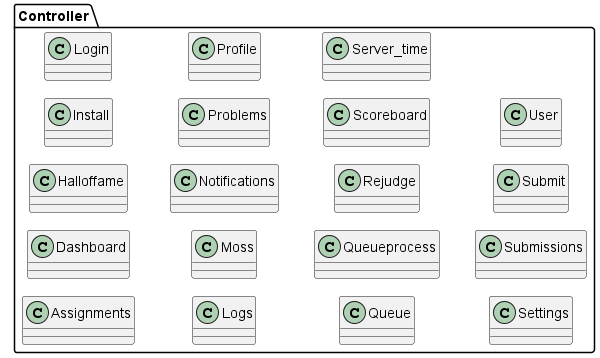
\includegraphics[width=0.65\textwidth]{analisis/class/class_controller.png}
		      \caption{Struktur Sederhana Controller pada SharIF Judge}
		      \label{fig:3:1:controller}
	      \end{figure}

	      \begin{figure}[H]
		      \centering
		      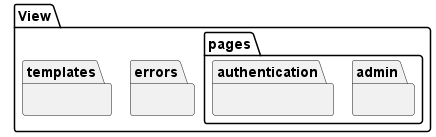
\includegraphics[width=0.5\textwidth]{analisis/class/class_view.png}
		      \caption{Struktur Sederhana View pada SharIF Judge}
		      \label{fig:3:1:view}
	      \end{figure}

	      Berikut merupakan hasil eksplorasi dari struktur MVC pada SharIF Judge:

	      \begin{itemize}
		      \item \textbf{Model}
		            \label{sub:3:1:1:model}

		            Hasil pembelajaran MVC akan dimulai dengan \textit{model} yang berada pada direktori \verb|application/mo|\\\verb|dels|. Direktori \textit{Model} berisi kelas-kelas yang digunakan untuk mengelola dan mengembalikan data dari \textit{database}. Gambar \ref{fig:3:1:1:model} merupakan struktur kelas \textit{model} dalam SharIF Judge.
		            \begin{figure}[H]
			            \centering
			            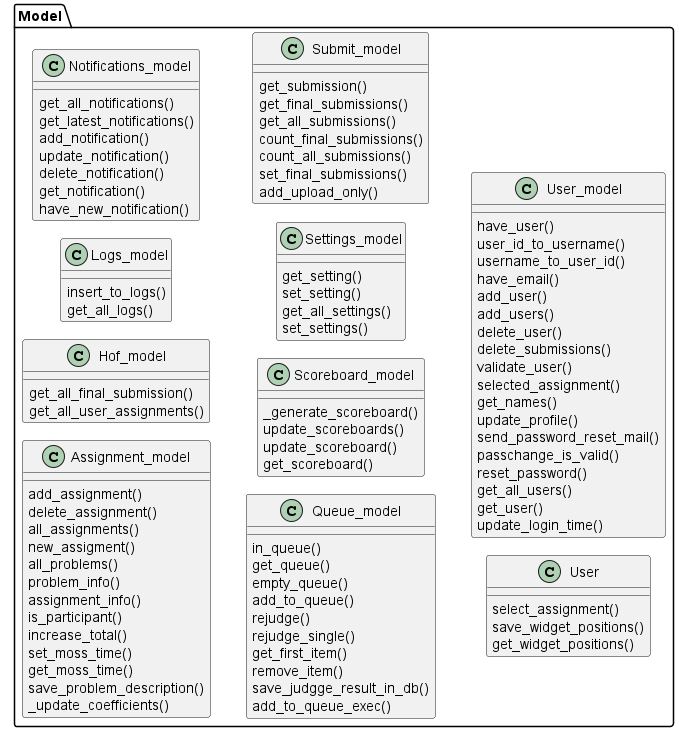
\includegraphics[width=0.95\textwidth]{analisis/mvc/model.png}
			            \caption{Struktur Kelas Model pada SharIF Judge}
			            \label{fig:3:1:1:model}
		            \end{figure}

		            \begin{figure}[H]
			            \centering
			            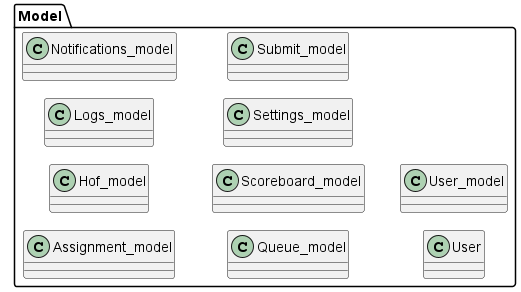
\includegraphics[width=0.9\textwidth]{analisis/class/class_model.png}
			            \caption{Struktur Sederhana Model pada SharIF Judge}
			            \label{fig:3:1:model}
		            \end{figure}

		            Berikut merupakan penjelasan dari kelas \textit{model} dan fungsi-fungsinya yang terdapat pada SharIF Judge:

		            \begin{itemize}
			            \item \verb|Assignment_model.php| \\
			                  Model ini digunakan untuk mengelola tabel \verb|assignments| dan mengembalikan informasi yang digunakan dalam halaman \textit{assignment} dan \textit{problem}. Fungsi yang dimiliki adalah sebagai berikut:

			                  \begin{itemize}
				                  \item \verb|add_assignment($id, $edit)| \\
				                        Menambahkan atau memperbaharui sebuah \textit{assignment}.
				                  \item \verb|delete_assignment($assignment_id)| \\
				                        Menghapus sebuah \textit{assignment}.
				                  \item \verb|all_assignments()| \\
				                        Mengembalikan daftar semua \textit{assignment} dan informasinya.
				                  \item \verb|new_assignment_id()| \\
				                        Mendapatkan nomor terkecil dan dapat digunakan sebagai \textit{id assignment} terbaru.
				                  \item \verb|all_problems($assignment_id)| \\
				                        Mengembalikan daftar semua \textit{problems} dari sebuah \textit{assignment}.
				                  \item \verb|problem_info($assignment_id, $problem_id)| \\
				                        Mengembalikan semua informasi sebuah \textit{problem}
				                  \item \verb|assignment_info($assignment_id)| \\
				                        Mengembalikan semua informasi sebuah \textit{assignment}
				                  \item \verb|is_participant($participants, $username)| \\
				                        Mengembalikan sebuah \verb|boolean| yang menyatakan bahwa \verb|$username| terdapat dalam \verb|$participants|.
				                  \item \verb|increase_total_submits($assignment_id)| \\
				                        Menambahkan jumlah \textit{total submits} sebanyak satu pada sebuah assignment.
				                  \item \verb|set_moss_time($assignment_id)| \\
				                        Memperbaharui ``\textit{Moss Update Time}'' pada sebuah \textit{assignment}.
				                  \item \verb|get_moss_time($assignment_id)| \\
				                        Mengembalikan ``\textit{Moss Update Time}'' pada sebuah assignment.
				                  \item \verb|save_problem_description($assignment_id, $problem_id, $text, $type)| \\
				                        Menambahkan atau memperbaharui deskripsi pada sebuah \textit{problem}.
				                  \item \verb|_update_coefficients($a_id, $extra_time, $finish_time, $new_late_rule)| \\
				                        Memperbaharui koefisien dari sebuah \textit{assignment}.
			                  \end{itemize}

			                  \vspace{0.5cm}
			            \item \verb|Hof_model.php| \\
			                  Model ini digunakan untuk mengembalikan informasi yang digunakan dalam \textit{hall of fame} dari tabel \verb|submissions|. Fungsi yang dimiliki adalah sebagai berikut:

			                  \begin{itemize}
				                  \item \verb|get_all_final_submission()| \\
				                        Mengembalikan seluruh total nilai \textit{final submission} untuk semua \textit{user}.
				                  \item \verb|get_all_user_assignments($username)| \\
				                        Mengembalikan nilai \textit{final submission} pada semua problem untuk \textit{user} tertentu.
			                  \end{itemize}

			                  \vspace{0.5cm}
			            \item \verb|Logs_model.php| \\
			                  Model ini berfungsi untuk mengelola tabel \verb|logins| dan mengembalikan catatan \textit{login}. Fungsi yang dimiliki adalah sebagai berikut:

			                  \begin{itemize}
				                  \item \verb|insert_to_logs($username, $ip_adrress)| \\
				                        Mencatat \textit{login} sebuah \textit{user} dan menghapus catatan jika melebihi 24 jam.
				                  \item \verb|get_all_logs()| \\
				                        Mengembalikan semua catatan \textit{login}.
			                  \end{itemize}

			                  \vspace{0.5cm}
			            \item \verb|Notifications_model.php| \\
			                  Model ini digunakan untuk mengelola tabel \verb|notifications|. Fungsi yang dimiliki oleh \textit{model} \verb|Notifications_model.php| adalah sebagai berikut:

			                  \begin{itemize}
				                  \item \verb|get_all_notifications()| \\
				                        Mengembalikan semua \textit{notifications}.
				                  \item \verb|get_latest_notifications()| \\
				                        Mengembalikan 10 \textit{notifications} terbaru.
				                  \item \verb|add_notification($title, $text)| \\
				                        Menambahkan \textit{notification} baru.
				                  \item \verb|update_notification($id, $title, $text)| \\
				                        Memperbaharui sebuah \textit{notification}.
				                  \item \verb|delete_notification($id)| \\
				                        Menghapus sebuah \textit{notification}.
				                  \item \verb|get_notification($notif_id)| \\
				                        Mengembalikan sebuah \textit{notification}.
				                  \item \verb|have_new_notification($time)| \\
				                        Mengembalikan sebuah \textit{boolean} yang menyatakan bahwa terdapatnya \textit{notification} baru.
			                  \end{itemize}

			                  \vspace{0.5cm}
			            \item \verb|Queue_model.php| \\
			                  Model ini digunakan untuk mengelola tabel \verb|queue| dan menampilkan data \verb|queue|. Fungsi yang dimiliki adalah sebagai berikut:

			                  \begin{itemize}
				                  \item \verb|in_queue($username, $assignment, $problem)| \\
				                        Fungsi ini digunakan untuk mengembalikan sebuah \textit{boolean} yang menyatakan bahwa \textit{username} masih memiliki \textit{queue} dalam sebuah \textit{problem}.
				                  \item \verb|get_queue()| \\
				                        Mengambil semua \textit{submission queue}.
				                  \item \verb|empty_queue()| \\
				                        Menghapus semua \textit{queue}.
				                  \item \verb|add_to_queue($submit_info)| \\
				                        Menambahkan sebuah \textit{submission} ke dalam \textit{queue}.
				                  \item \verb|rejudge($assignment_id, $problem_id)| \\
				                        Fungsi ini digunakan untuk menambahkan seluruh \textit{submissions} dalam sebuah \textit{problem} ke dalam \textit{queue} untuk dinilai ulang.
				                  \item \verb|rejudge_single($submission)| \\
				                        Menambahkan sebuah \textit{submission} ke dalam \textit{queue} untuk dinilai ulang.
				                  \item \verb|get_first_item()| \\
				                        Mengembalikan \textit{item} pertama dalam tabel \verb|queue|.
				                  \item \verb|remove_item($username, $assignment, $problem, $submit_id)| \\
				                        Menghapus sebuah \textit{item} tertentu dalam tabel \verb|queue|.
				                  \item \verb|save_judge_result_in_db ($submission, $type)| \\
				                        Menyimpan hasil penilaian \textit{judge} ke dalam \textit{database}.
				                  \item \verb|add_to_queue_exec($submit_info)| \\
				                        Fungsi ini digunakan untuk menambahkan sebuah \textit{dummy submission} yang digunakan hanya untuk dijalankan ke dalam \textit{queue}.
			                  \end{itemize}

			                  \vspace{0.5cm}
			            \item \verb|Scoreboard_model.php| \\
			                  Model ini digunakan untuk mengelola tabel \verb|scoreboard|. Fungsi yang dimiliki oleh \textit{model} \verb|Scoreboard_model.php| adalah sebagai berikut:

			                  \begin{itemize}
				                  \item \verb|_generate_scoreboard($assignment_id)| \\
				                        Menghasilkan \textit{scoreboard} untuk sebuah \textit{assignment} dari nilai akhir semua \textit{submission}.
				                  \item \verb|update_scoreboards()| \\
				                        Memperbaharui \textit{scoreboard} untuk semua \textit{assignment}.
				                  \item \verb|update_scoreboard($assignment_id)| \\
				                        Memperbaharui \textit{scoreboard} untuk sebuah \textit{assignment}.
				                  \item \verb|get_scoreboard($assignment_id)| \\
				                        Mengembalikan \textit{scoreboard} pada sebuah \textit{assignment}.
			                  \end{itemize}

			                  \vspace{0.5cm}
			            \item \verb|Settings_model.php| \\
			                  Model ini digunakan untuk mengelola tabel \verb|settings|. Fungsi yang dimiliki oleh \textit{model} \\\verb|Settings_model.php| adalah sebagai berikut:

			                  \begin{itemize}
				                  \item \verb|get_setting($key)| \\
				                        Mengembalikan nilai dari sebuah \verb|$key| pada tabel \verb|settings|.
				                  \item \verb|set_setting($key, $value)| \\
				                        Memperbaharui nilai dari pada \textit{setting} \verb|$key|.
				                  \item \verb|get_all_settings()| \\
				                        Mengembalikan seluruh \textit{settings}.
				                  \item \verb|set_settings($settings)| \\
				                        Memperbaharui seluruh nilai perubahan \textit{settings}.
			                  \end{itemize}

			                  \vspace{0.5cm}
			            \item \verb|Submit_model.php| \\
			                  Model ini digunakan untuk mengelola tabel \verb|submission|. Fungsi yang dimiliki oleh \textit{model} \verb|Submit_model.php| adalah sebagai berikut:

			                  \begin{itemize}
				                  \item \verb|get_submission($username, $assignment, $problem, $submit_id)| \\
				                        Mengembalikan sebuah baris data \textit{submission} tertentu.
				                  \item \verb|get_final_submissions($a_id, $u_vl, $uname, $p_num, $fil_u, $fil_prob)| \\
				                        Mengembalikan seluruh \textit{final submission} pada sebuah \textit{assignment}. \textit{User} dengan role \textit{student} hanya dapat melihat \textit{final submission} dirinya sendiri.
				                  \item \verb|get_all_submissions($a_id, $u_vl, $uname, $p_num, $fil_u, $fil_prob)| \\
				                        Mengembalikan seluruh \textit{submission} pada sebuah \textit{assignment}. \textit{User} dengan role \textit{student} hanya dapat melihat \textit{submission} dirinya sendiri.
				                  \item \verb|count_final_submissions($a_id, $u_vl, $uname, $fil_u, $fil_prob)| \\
				                        Mengembalikan jumlah \textit{final submission} pada sebuah \textit{assignment}.
				                  \item \verb|count_all_submissions($a_id, $u_vl, $uname, $fil_u, $fil_prob)| \\
				                        Mengembalikan jumlah \textit{submission} pada sebuah \textit{assignment}.
				                  \item \verb|set_final_submission($username, $assignment, $problem, $submit_id)| \\
				                        Memperbaharui sebuah \textit{submission} menjadi \textit{final submission}.
				                  \item \verb|add_upload_only($submit_info)| \\
				                        Menyimpan hasil \textit{upload only problem} ke dalam tabel \textit{database}.
			                  \end{itemize}

			                  \vspace{0.5cm}
			            \item \verb|User.php| \\
			                  Model ini digunakan untuk menyimpan \textit{settings} sebuah \textit{user}. Fungsi yang dimiliki oleh \textit{model} \verb|User.php| adalah sebagai berikut:

			                  \begin{itemize}
				                  \item \verb|select_assignment($assignment_id)| \\
				                        Menyimpan \textit{assignment} yang dipilih oleh \textit{user}.
				                  \item \verb|save_widget_positions($positions)| \\
				                        Menyimpan posisi \textit{widget} sebuah \textit{user}.
				                  \item \verb|get_widget_positions()| \\
				                        Mendapatkan posisi \textit{widget} sebuah \textit{user}.
			                  \end{itemize}

			                  \vspace{0.5cm}
			            \item \verb|User_model.php| \\
			                  Model \verb|User_model.php| digunakan untuk mengelola tabel \verb|users|. Fungsi yang dimiliki oleh \textit{model} \verb|User_model.php| adalah sebagai berikut:

			                  \begin{itemize}
				                  \item \verb|have_user($username)| \\
				                        Mengembalikan sebuah \textit{boolean} yang menyatakan \verb|$username| sudah ada pada \textit{database}.
				                  \item \verb|user_id_to_username($user_id)| \\
				                        Mengembalikan \textit{username} dari \verb|$user_id|.
				                  \item \verb|username_to_user_id($username)| \\
				                        Mengembalikan \textit{user id} dari \verb|$username|.
				                  \item \verb|have_email($email, $username)| \\
				                        Mengembalikan sebuah \textit{boolean} yang menyatakan jika \textit{user} memiliki \textit{email} pada \textit{database}.
				                  \item \verb|add_user($username, $email, $display_name, $password, $role)| \\
				                        Menambahkan satu \textit{user} baru ke dalam \textit{database}.
				                  \item \verb|add_users($text, $send_mail, $delay)| \\
				                        Menambahkan banyak \textit{user} baru ke dalam \textit{database}.
				                  \item \verb|delete_user($user_id)| \\
				                        Menghapus sebuah \textit{user} dalam \textit{database}.
				                  \item \verb|delete_submissions($user_id)| \\
				                        Mendelete semua \textit{submissions} yang di \textit{submit} oleh sebuah \textit{user}.
				                  \item \verb|validate_user($username, $password)| \\
				                        Mengembalikan sebuah \textit{boolean} yang menyatakan bahwa \verb|$password| dan \verb|$username|
				                  \item \verb|selected_assignment($username)| \\
				                        Mengembalikan \textit{assignment} yang dipilih oleh \verb|$username|.
				                  \item \verb|get_names()| \\
				                        Mengembalikan semua \textit{display name} pada tabel \textit{users}.
				                  \item \verb|update_profile($user_id)| \\
				                        Memperbaharui nama, email, password, atau role sebuah \textit{user}.
				                  \item \verb|send_password_reset_mail($email)| \\
				                        Mengirimkan \textit{link reset password} ke email \textit{user} yang dapat dipakai selama 1 jam.
				                  \item \verb|passchange_is_valid($passchange_key)| \\
				                        Mengembalikan sebuah \textit{boolean} yang menyatakan bahwa \textit{link reset password} masih dapat dipakai.
				                  \item \verb|reset_password($passchange_key, $newpassword)| \\
				                        Memperbaharui \textit{password} dengan divalidasinya \textit{password change key}.
				                  \item \verb|get_all_users()| \\
				                        Mengembalikan seluruh \textit{user} pada tabel \verb|users|.
				                  \item \verb|get_user($user_id)| \\
				                        Mengembalikan sebuah \textit{user} yang memiliki id \verb|$user_id|.
				                  \item \verb|update_login_time($username)| \\
				                        Memperbaharui catatan \textit{login} untuk sebuah \textit{user}.
			                  \end{itemize}
		            \end{itemize}

		      \item \textbf{View}
		            \label{sub:3:1:1:view}

		            \textit{View} merupakan tampilan yang menjadi perantara antara pengguna dan \textit{sistem}. Pada SharIF Judge, \textit{View} disimpan pada direktori \verb|application/views| dan dibagi menjadi 3 direktori terpisah yaitu errors, pages, dan template.
		            Gambar \ref{fig:3:1:1:view} merupakan struktur direktori \textit{view} beserta \textit{view} yang terdapat pada direktorinya dalam SharIF Judge.
		            \begin{figure}[H]
			            \centering
			            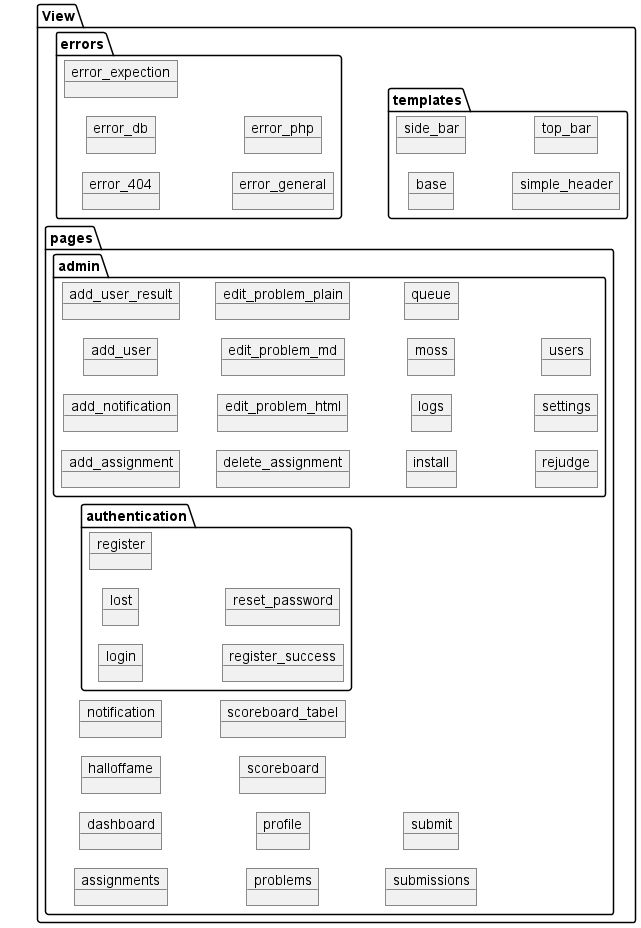
\includegraphics[width=0.65\textwidth]{analisis/mvc/view.png}
			            \caption{Struktur Direktori View pada SharIF Judge}
			            \label{fig:3:1:1:view}
		            \end{figure}
		            Berikut merupakan penjelasan mengenai direktori penyimpanan untuk \textit{view} pada SharIF Judge.

		            \begin{itemize}
			            \item \verb|errors| \\
			                  Pada direktori \textit{errors}, berisi tampilan halaman \textit{error} jika terjadi error pada pengunaan SharIF Judge. Berikut merupakan \textit{views} yang terdapat pada direktori \verb|errors|:

			                  \begin{itemize}
				                  \item \verb|error_404|
				                  \item \verb|error_db|
				                  \item \verb|error_expection|
				                  \item \verb|error_general|
				                  \item \verb|error_php|
			                  \end{itemize}

			            \item \verb|pages| \\
			                  Pada direktori \textit{pages}, berisi tampilan halaman-halaman utama. \textit{pages} juga memiliki dua direktori selain halaman-halama. Berikut merupakan \textit{views} dan direktori yang terdapat pada direktori \verb|pages|:

			                  \begin{itemize}
				                  \item \verb|pages/admin| \\
				                        Direktori \textit{admin} berisi tampilan halaman khusus untuk \textit{role admin}. Berikut merupakan \textit{views} yang terdapat pada direktori \verb|admin|:

				                        \begin{itemize}
					                        \item \verb|add_assignment.twig|
					                        \item \verb|add_notification.twig|
					                        \item \verb|add_user.twig|
					                        \item \verb|add_user_result.twig|
					                        \item \verb|delete_assignment.twig|
					                        \item \verb|edit_problem_html.twig|
					                        \item \verb|edit_problem_md.twig|
					                        \item \verb|edit_problem_plain.twig|
					                        \item \verb|install.twig|
					                        \item \verb|logs.twig|
					                        \item \verb|moss.twig|
					                        \item \verb|queue.twig|
					                        \item \verb|rejudge.twig|
					                        \item \verb|settings.twig|
					                        \item \verb|users.twig|
				                        \end{itemize}

				                        \vspace{0.25cm}
				                  \item \verb|pages/authentication| \\
				                        Direktori \textit{authentication} berisi tampilan halaman khusus untuk \textit{authentication} seperti halaman direktori \textit{Login}. Berikut merupakan \textit{views} yang terdapat pada direktori \verb|admin|:

				                        \begin{itemize}
					                        \item \verb|login.twig|
					                        \item \verb|lost.twig|
					                        \item \verb|register.twig|
					                        \item \verb|register_success.twig|
					                        \item \verb|reset_password.twig|
				                        \end{itemize}

				                  \item \verb|assignments.twig|
				                  \item \verb|dashboard.twig|
				                  \item \verb|halloffame.twig|
				                  \item \verb|notification.twig|
				                  \item \verb|problems.twig|
				                  \item \verb|profile.twig|
				                  \item \verb|scoreboard.twig|
				                  \item \verb|scoreboard_tabel.twig|
				                  \item \verb|submissions.twig|
				                  \item \verb|submit.twig|
			                  \end{itemize}

			                  \vspace{0.25cm}

			            \item \verb|templates| \\
			                  Pada direktori \textit{templates}, berisikan tampilan yang digunakan berulang oleh halaman utama seperti \textit{header} dan \textit{side bar}. Berikut merupakan \textit{views} yang terdapat pada direktori \verb|templates|:

			                  \begin{itemize}
				                  \item \verb|base.twig|
				                  \item \verb|side_bar.twig|
				                  \item \verb|simple_header.twig|
				                  \item \verb|top_bar.twig|
			                  \end{itemize}

		            \end{itemize}

		            \newpage

		      \item \textbf{Controller}
		            \label{sub:3:1:1:controller}

		            Pada bagian MVC terakhir, terdapat \textit{controller} yang berada pada direktori \verb|application/| \\ \verb|controller|. Seperti yang dijelaskan pada bagian \ref{sub:2:2:3:Controller}, \textit{Controller} digunakan sebagai perantara antara \textit{model}, \textit{view}, dan \textit{resources} lainnya yang dibutuhkan saat membuat sebuah web page. Direktori controller berisi kelas-kelas yang akan mengolah data yang didapat pada \textit{model} dan menyatukan data tersebut ke dalam \textit{views} yang akan ditampilkan kepada pengguna. Pada setiap kelas \textit{controller}, terdapat fungsi \verb|index()| yang menjadi fungsi utama saat kelas di akses oleh pengguna.
		            Gambar \ref{fig:3:1:1:controller} merupakan struktur kelas \textit{controller} yang terdapat pada SharIF Judge.
		            \begin{figure}[H]
			            \centering
			            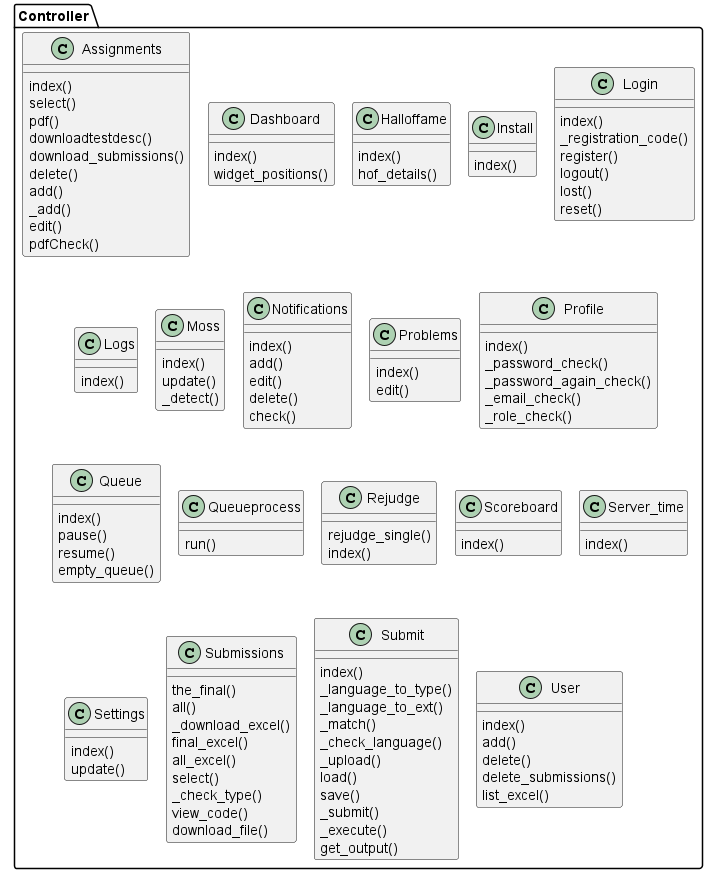
\includegraphics[width=0.65\textwidth]{analisis/mvc/controller.png}
			            \caption{Struktur Kelas Controller pada SharIF Judge}
			            \label{fig:3:1:1:controller}
		            \end{figure}
		            Berikut merupakan file \textit{controller} dan penjelasan fungsi-fungsinya yang terdapat pada SharIF Judge:

		            \begin{itemize}
			            \item \verb|Assignments.php| \\
			                  Berikut fungsi dengan penjelasannya pada \textit{controller} \verb|Assignments.php|:

			                  \begin{itemize}
				                  \item \verb|index()| \\
				                        Mengambil data dari \verb|Assignment_model| dan menaruh data dan mengembalikan \textit{views} \verb|assignments.twig|. Gambar \ref{fig:3:1:1:assignments} menunjukkan hasil halaman Assignment.

				                        \begin{figure}[H]
					                        \centering
					                        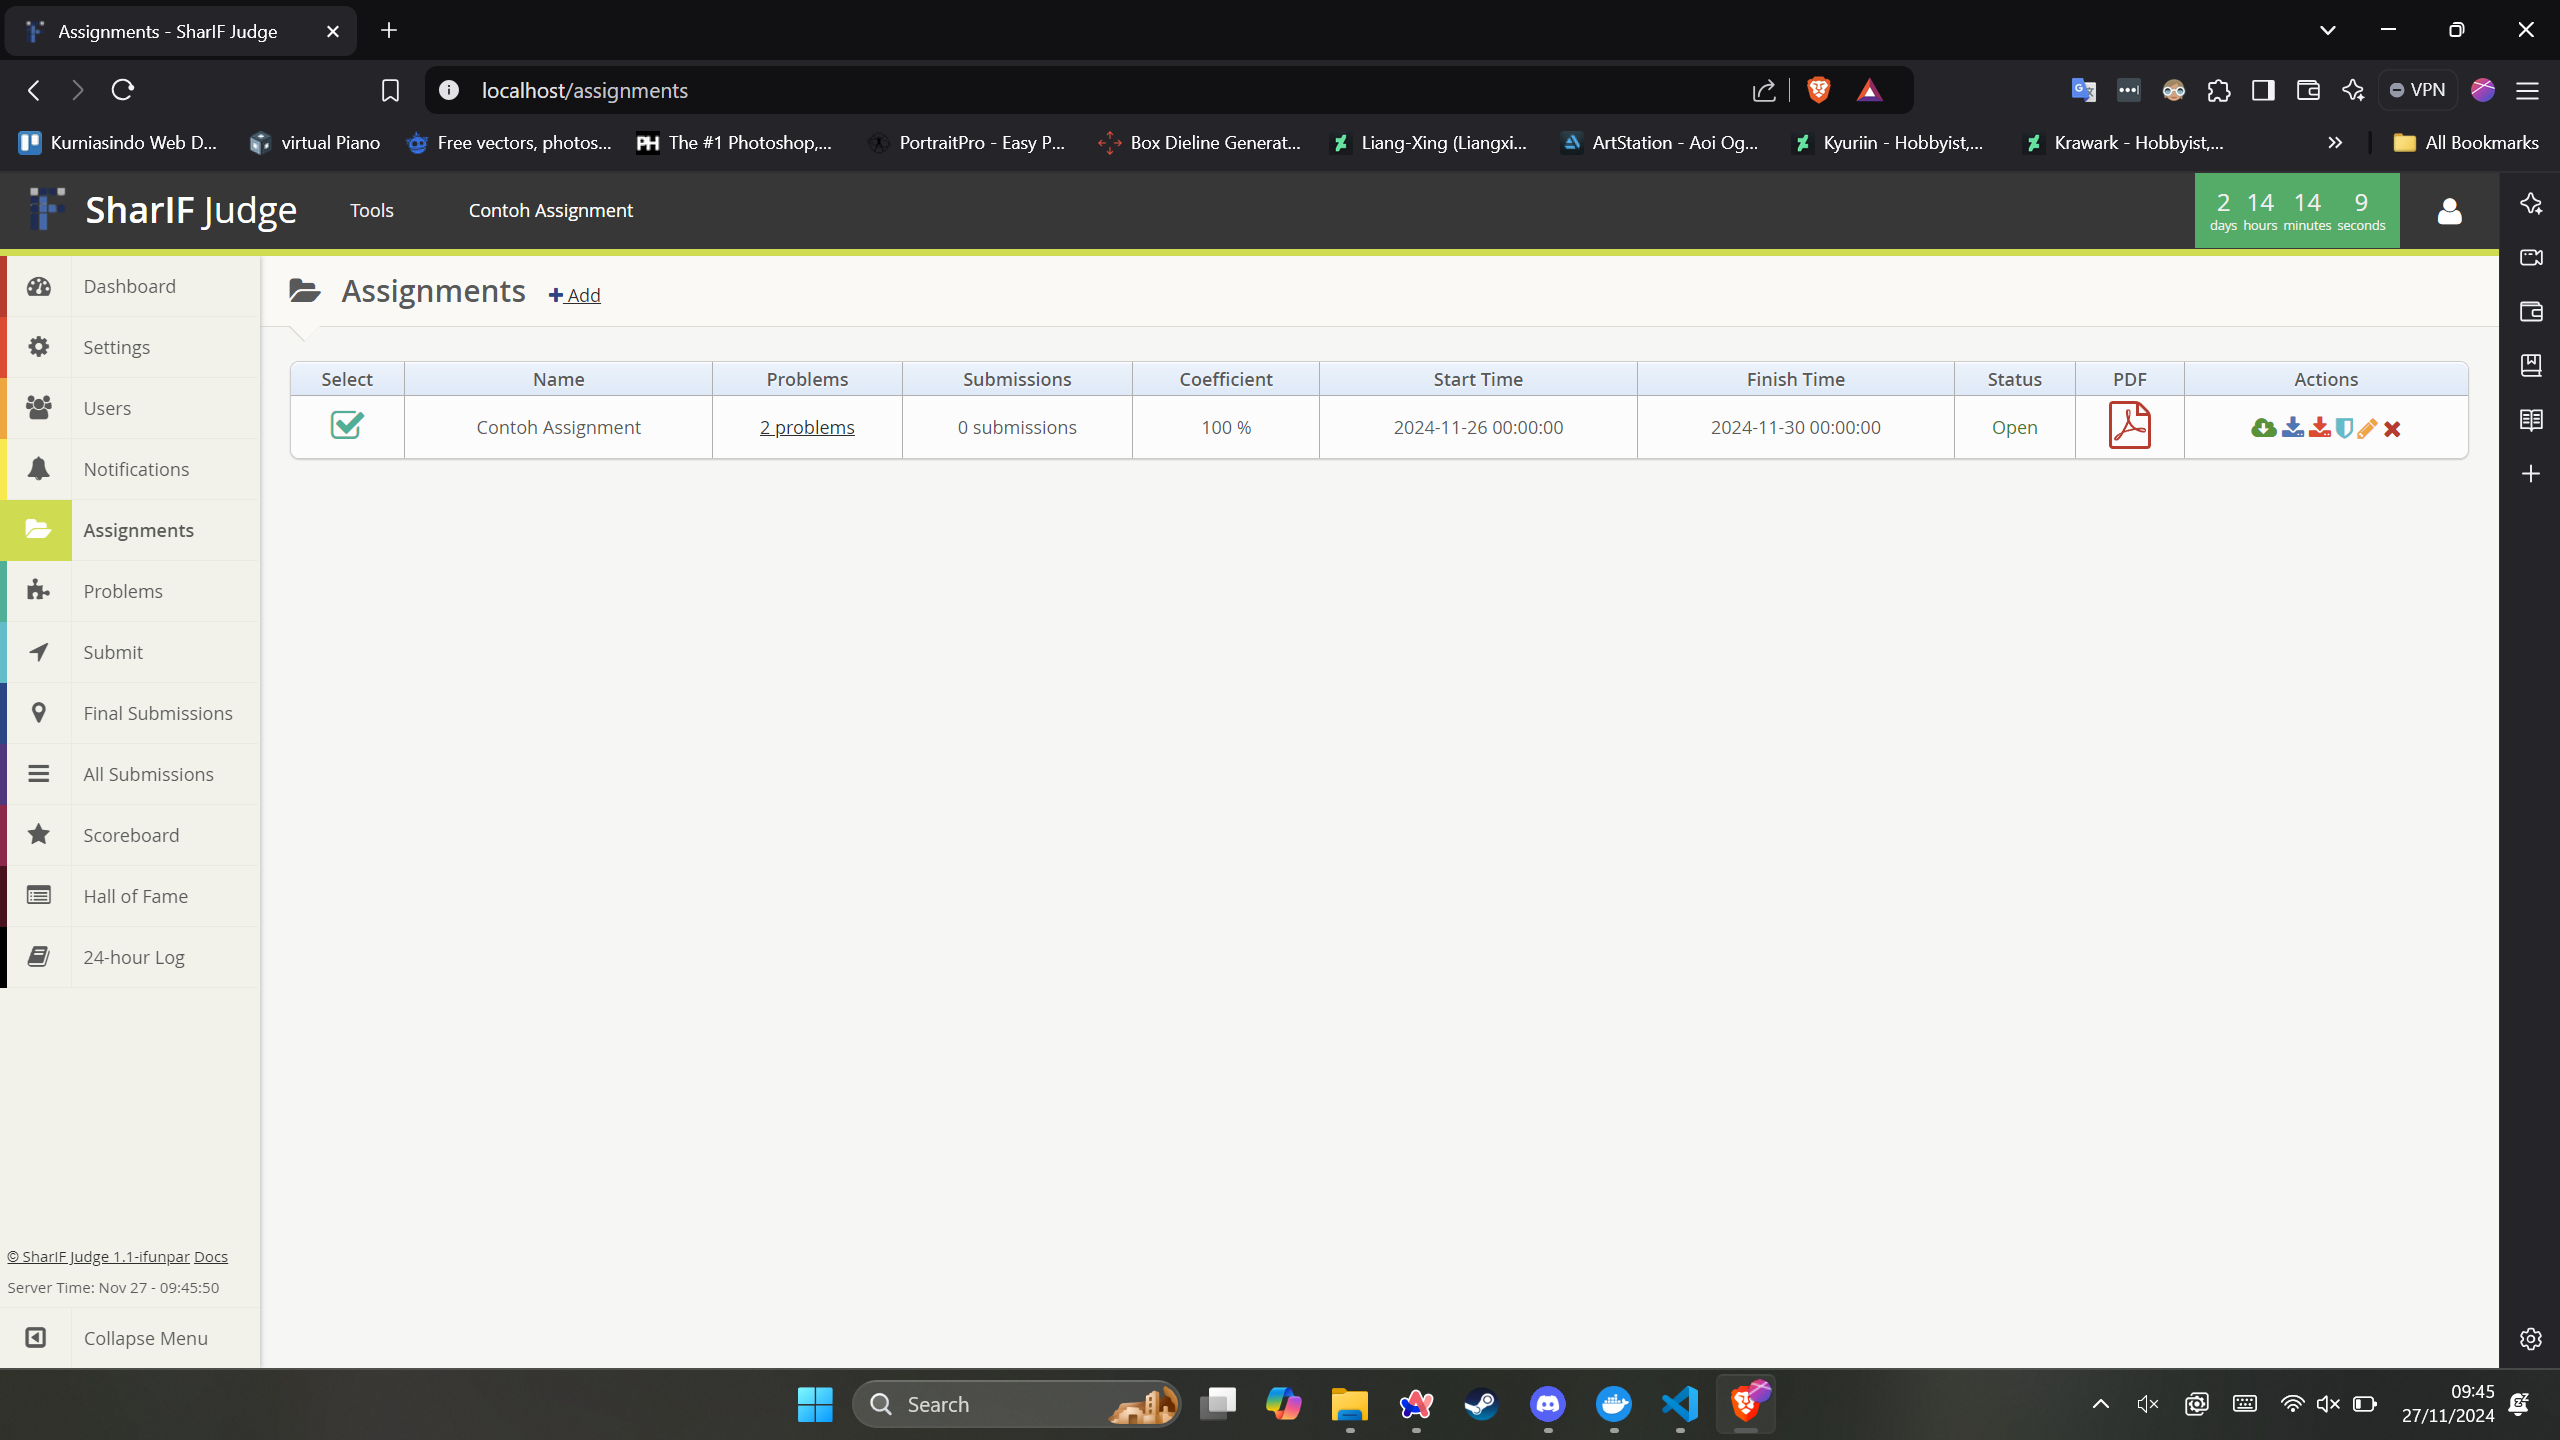
\includegraphics[width=0.8\textwidth]{views/assignments.png}
					                        \caption{Halaman Assignments}
					                        \label{fig:3:1:1:assignments}
				                        \end{figure}
				                  \item \verb|select()| \\
				                        Memilih \textit{assignment} yang ditampilkan pada \textit{top bar} menggunakan \textit{ajax request}.
				                  \item \verb|pdf($assignment_id, $problem_id, $no_download)| \\
				                        Mengunduh \textit{assignment} atau \textit{problem} dalam bentuk \textit{pdf file} ke browser.
				                  \item \verb|downloadtestsdesc($assignment_id)| \\
				                        Mengunduh dan mencompress data uji dan deskripsi sebuah \textit{assignment}.
				                  \item \verb|download_submissions($type, $assignment_id)| \\
				                        Mengunduh semua \textit{final submission} pada semua \textit{assignment}.
				                  \item \verb|delete($assignment_id)| \\
				                        Menghapus sebuah \textit{assignment}.
				                  \item \verb|add()| \\
				                        Mendapatkan \textit{input} dari pengguna dan mengirimkan \textit{input} pada fungsi \verb|_add()|.
				                  \item \verb|_add()| \\
				                        Menambahkan atau memperbaharui sebuah \textit{assignment}.
				                  \item \verb|edit($assignment_id)| \\
				                        Menandai \textit{assignment} yang akan di \textit{edit} dan memanggil fungsi \verb|add|.
				                  \item \verb|pdfCheck($assignment_id, $problem_id)| \\
				                        Melakukan validasi ketersediaan pdf pada sebuah \textit{assignment} atau pada sebuah \textit{problem}.
			                  \end{itemize}

			            \item \verb|Dashboard.php| \\
			                  Berikut fungsi dengan penjelasannya pada \textit{controller} \verb|Dashboard.php|:

			                  \begin{itemize}
				                  \item \verb|index()| \\
				                        Mendapatkan data dari beberapa model yaitu \verb|Assignment_model|, \verb|Settings_model|, \verb|User|, dan \verb|Notifications_model|. Data akan dimasukkan ke dalam \verb|dashboard.twig| yang akan dikembalikan ke pengguna. Gambar \ref{fig:3:1:1:dashboard} menunjukkan hasil halaman Dashboard yang dapat diakses oleh semua \textit{role}.

				                        \begin{figure}[H]
					                        \centering
					                        \includegraphics[width=0.75\textwidth]{views/dashboard.png}
					                        \caption{Halaman Dashboard}
					                        \label{fig:3:1:1:dashboard}
					                        \vspace{-0.25cm}
				                        \end{figure}


				                  \item \verb|widget_positions()| \\
				                        Mengunakan \textit{ajax request} untuk menyimpan posisi \textit{widget}.


			                  \end{itemize}

			            \item \verb|Halloffame.php| \\
			                  Berikut fungsi dengan penjelasannya pada \textit{controller} \verb|Halloffame.php|:

			                  \begin{itemize}
				                  \item \verb|index()| \\
				                        Mendapatkan data dari \verb|Hof_model| dan mengembalikan \textit{view} \verb|halloffame.twig|. Gambar \ref{fig:3:1:1:hof} menunjukkan hasil halaman Hall of Fame yang dapat diakses oleh semua \textit{role}.

				                        \begin{figure}[H]
					                        \centering
					                        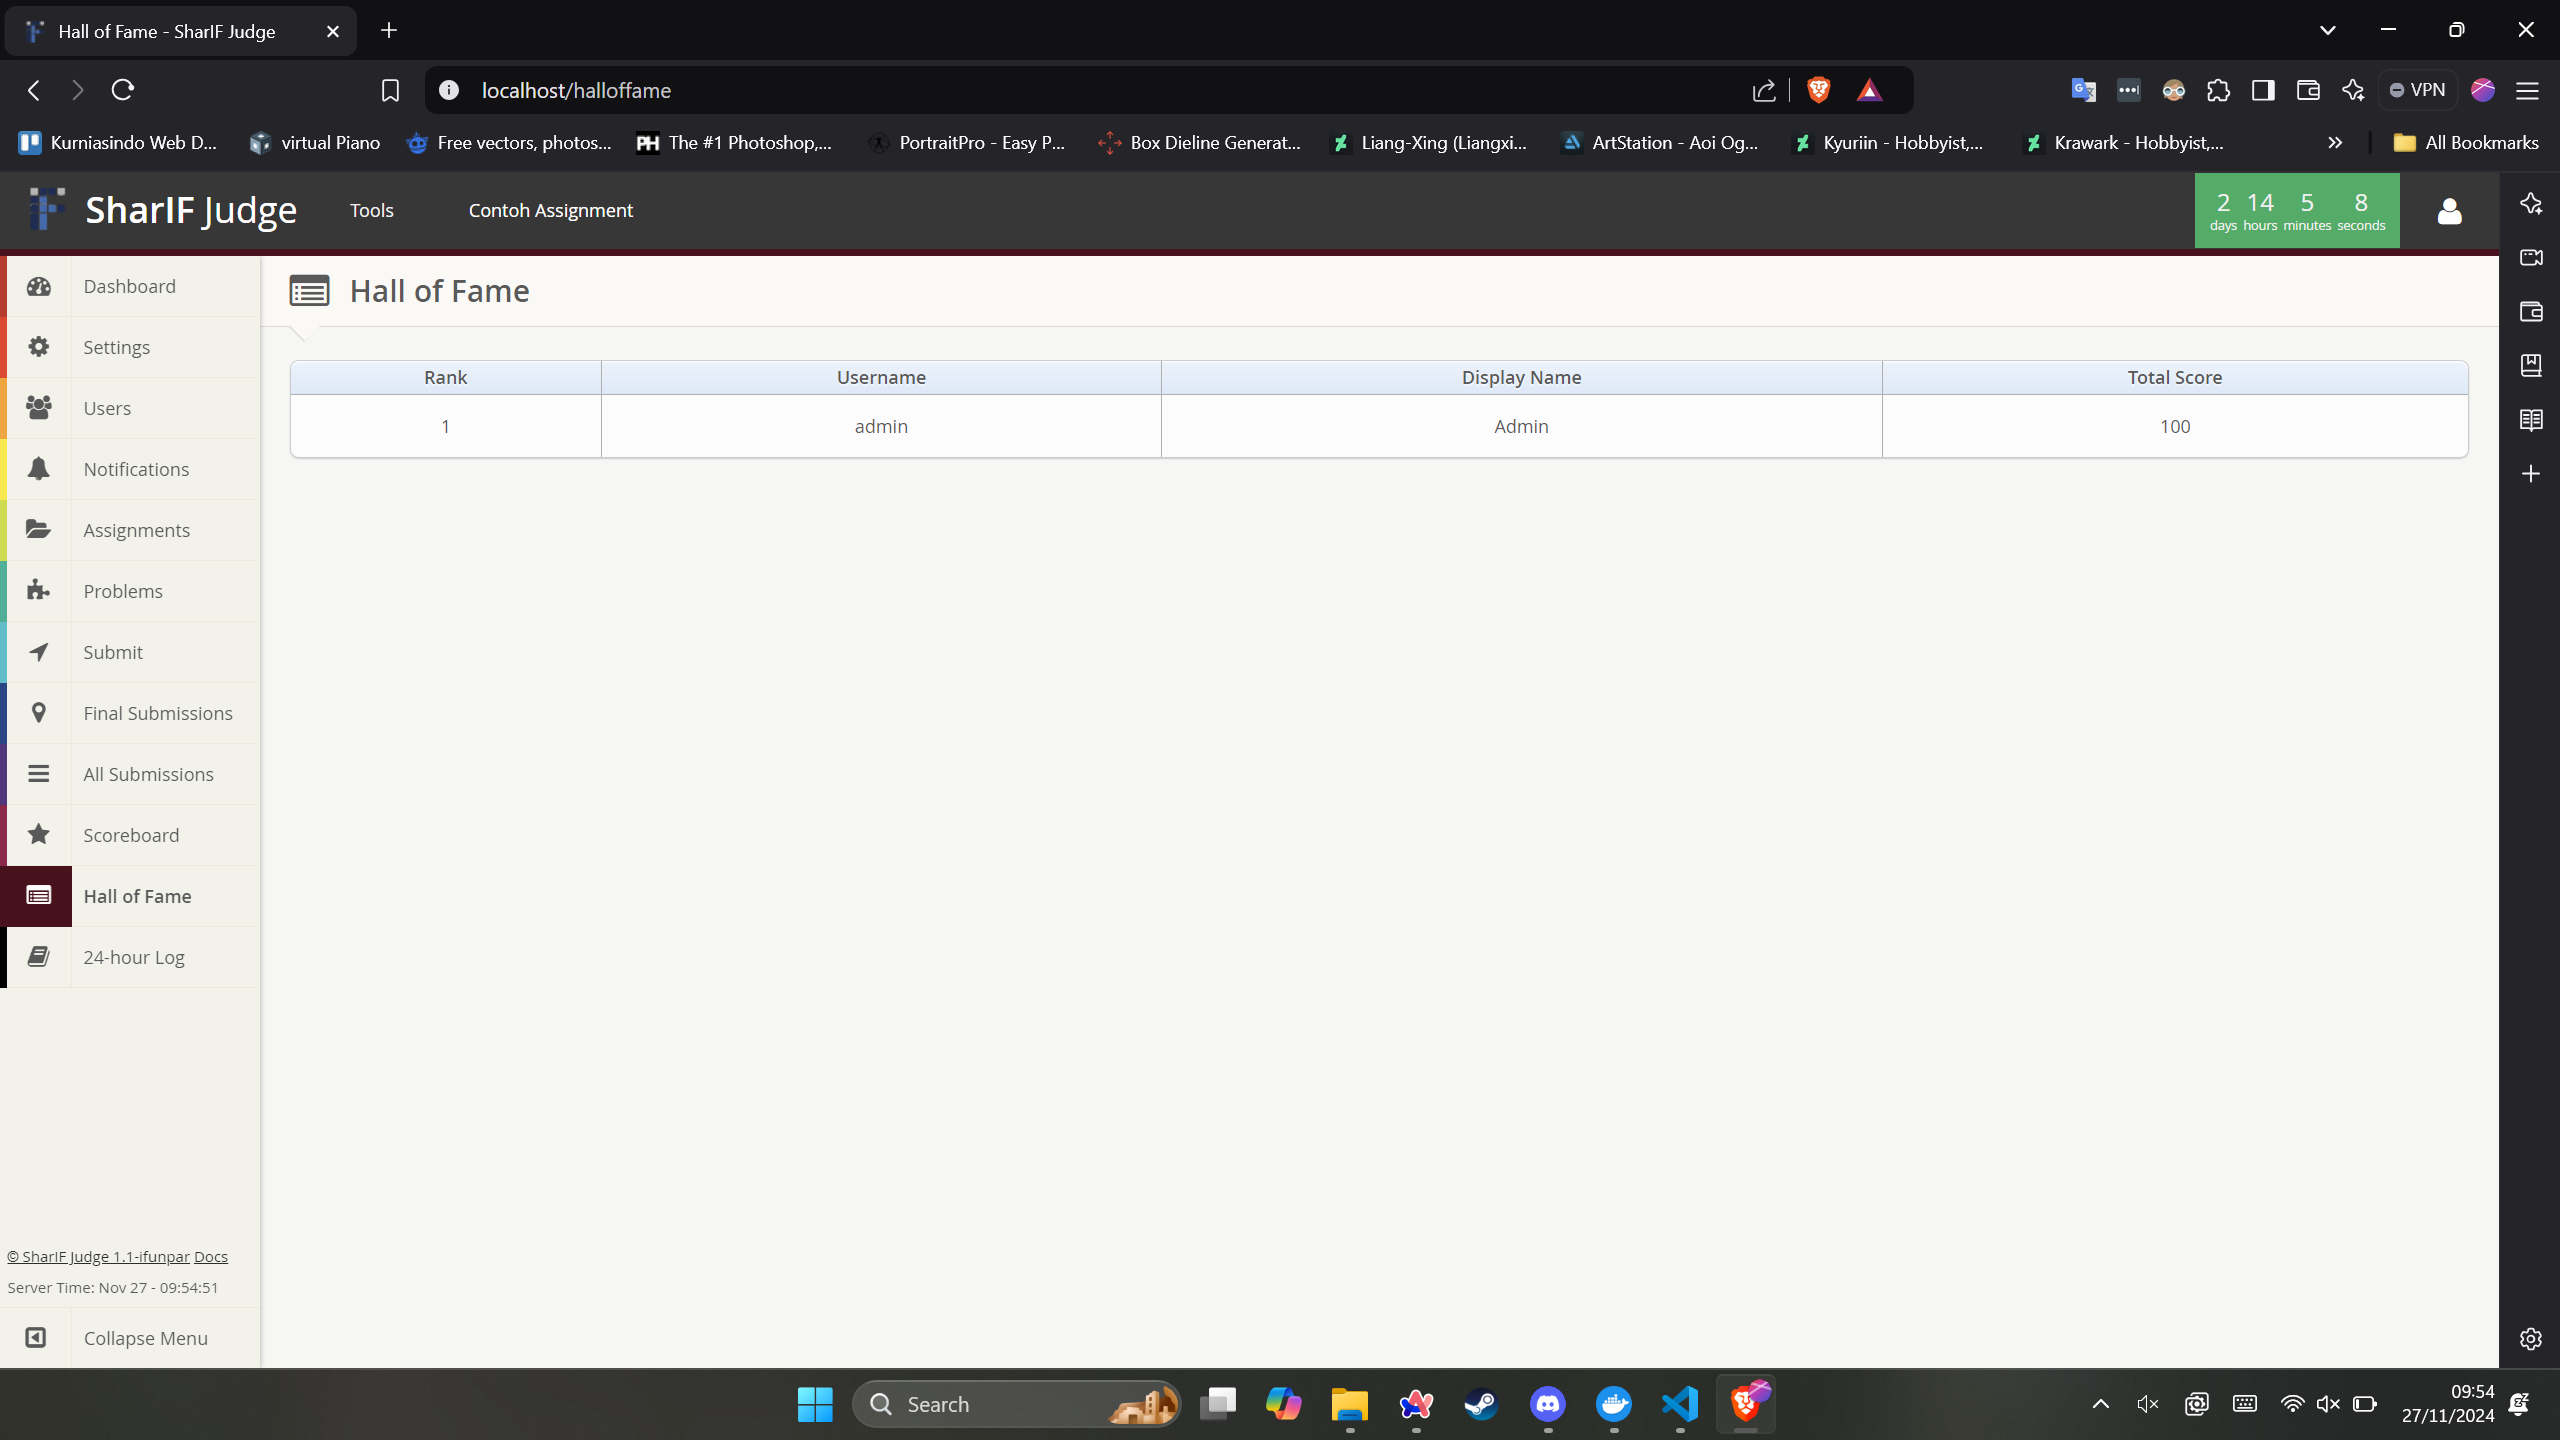
\includegraphics[width=0.75\textwidth]{views/hof.png}
					                        \caption{Halaman Hall of Fame}
					                        \label{fig:3:1:1:hof}
					                        % \vspace{-1.1cm}
				                        \end{figure}

				                  \item \verb|hof_details()| \\
				                        Menampilkan nilai akhir semua \textit{problem} dan \textit{assignments} pada sebuah \textit{user}.

			                  \end{itemize}

			            \item \verb|Install.php| \\
			                  Pada \textit{controller} \verb|Install.php| hanya ada satu fungsi yang menangani pembuatan seluruh tabel pada \textit{database} yang dibutuhkan oleh SharIF Judge. Setelah membuat \textit{database} akan mengembalikan \textit{view} \verb|install.twig| yang dapat diisi oleh pengguna tentang data \textit{user} dengan role \textit{admin} saat \textit{form} di kirim. Gambar \ref{fig:3:1:1:install} menunjukkan hasil halaman Install.

			                  \begin{figure}[H]
				                  \centering
				                  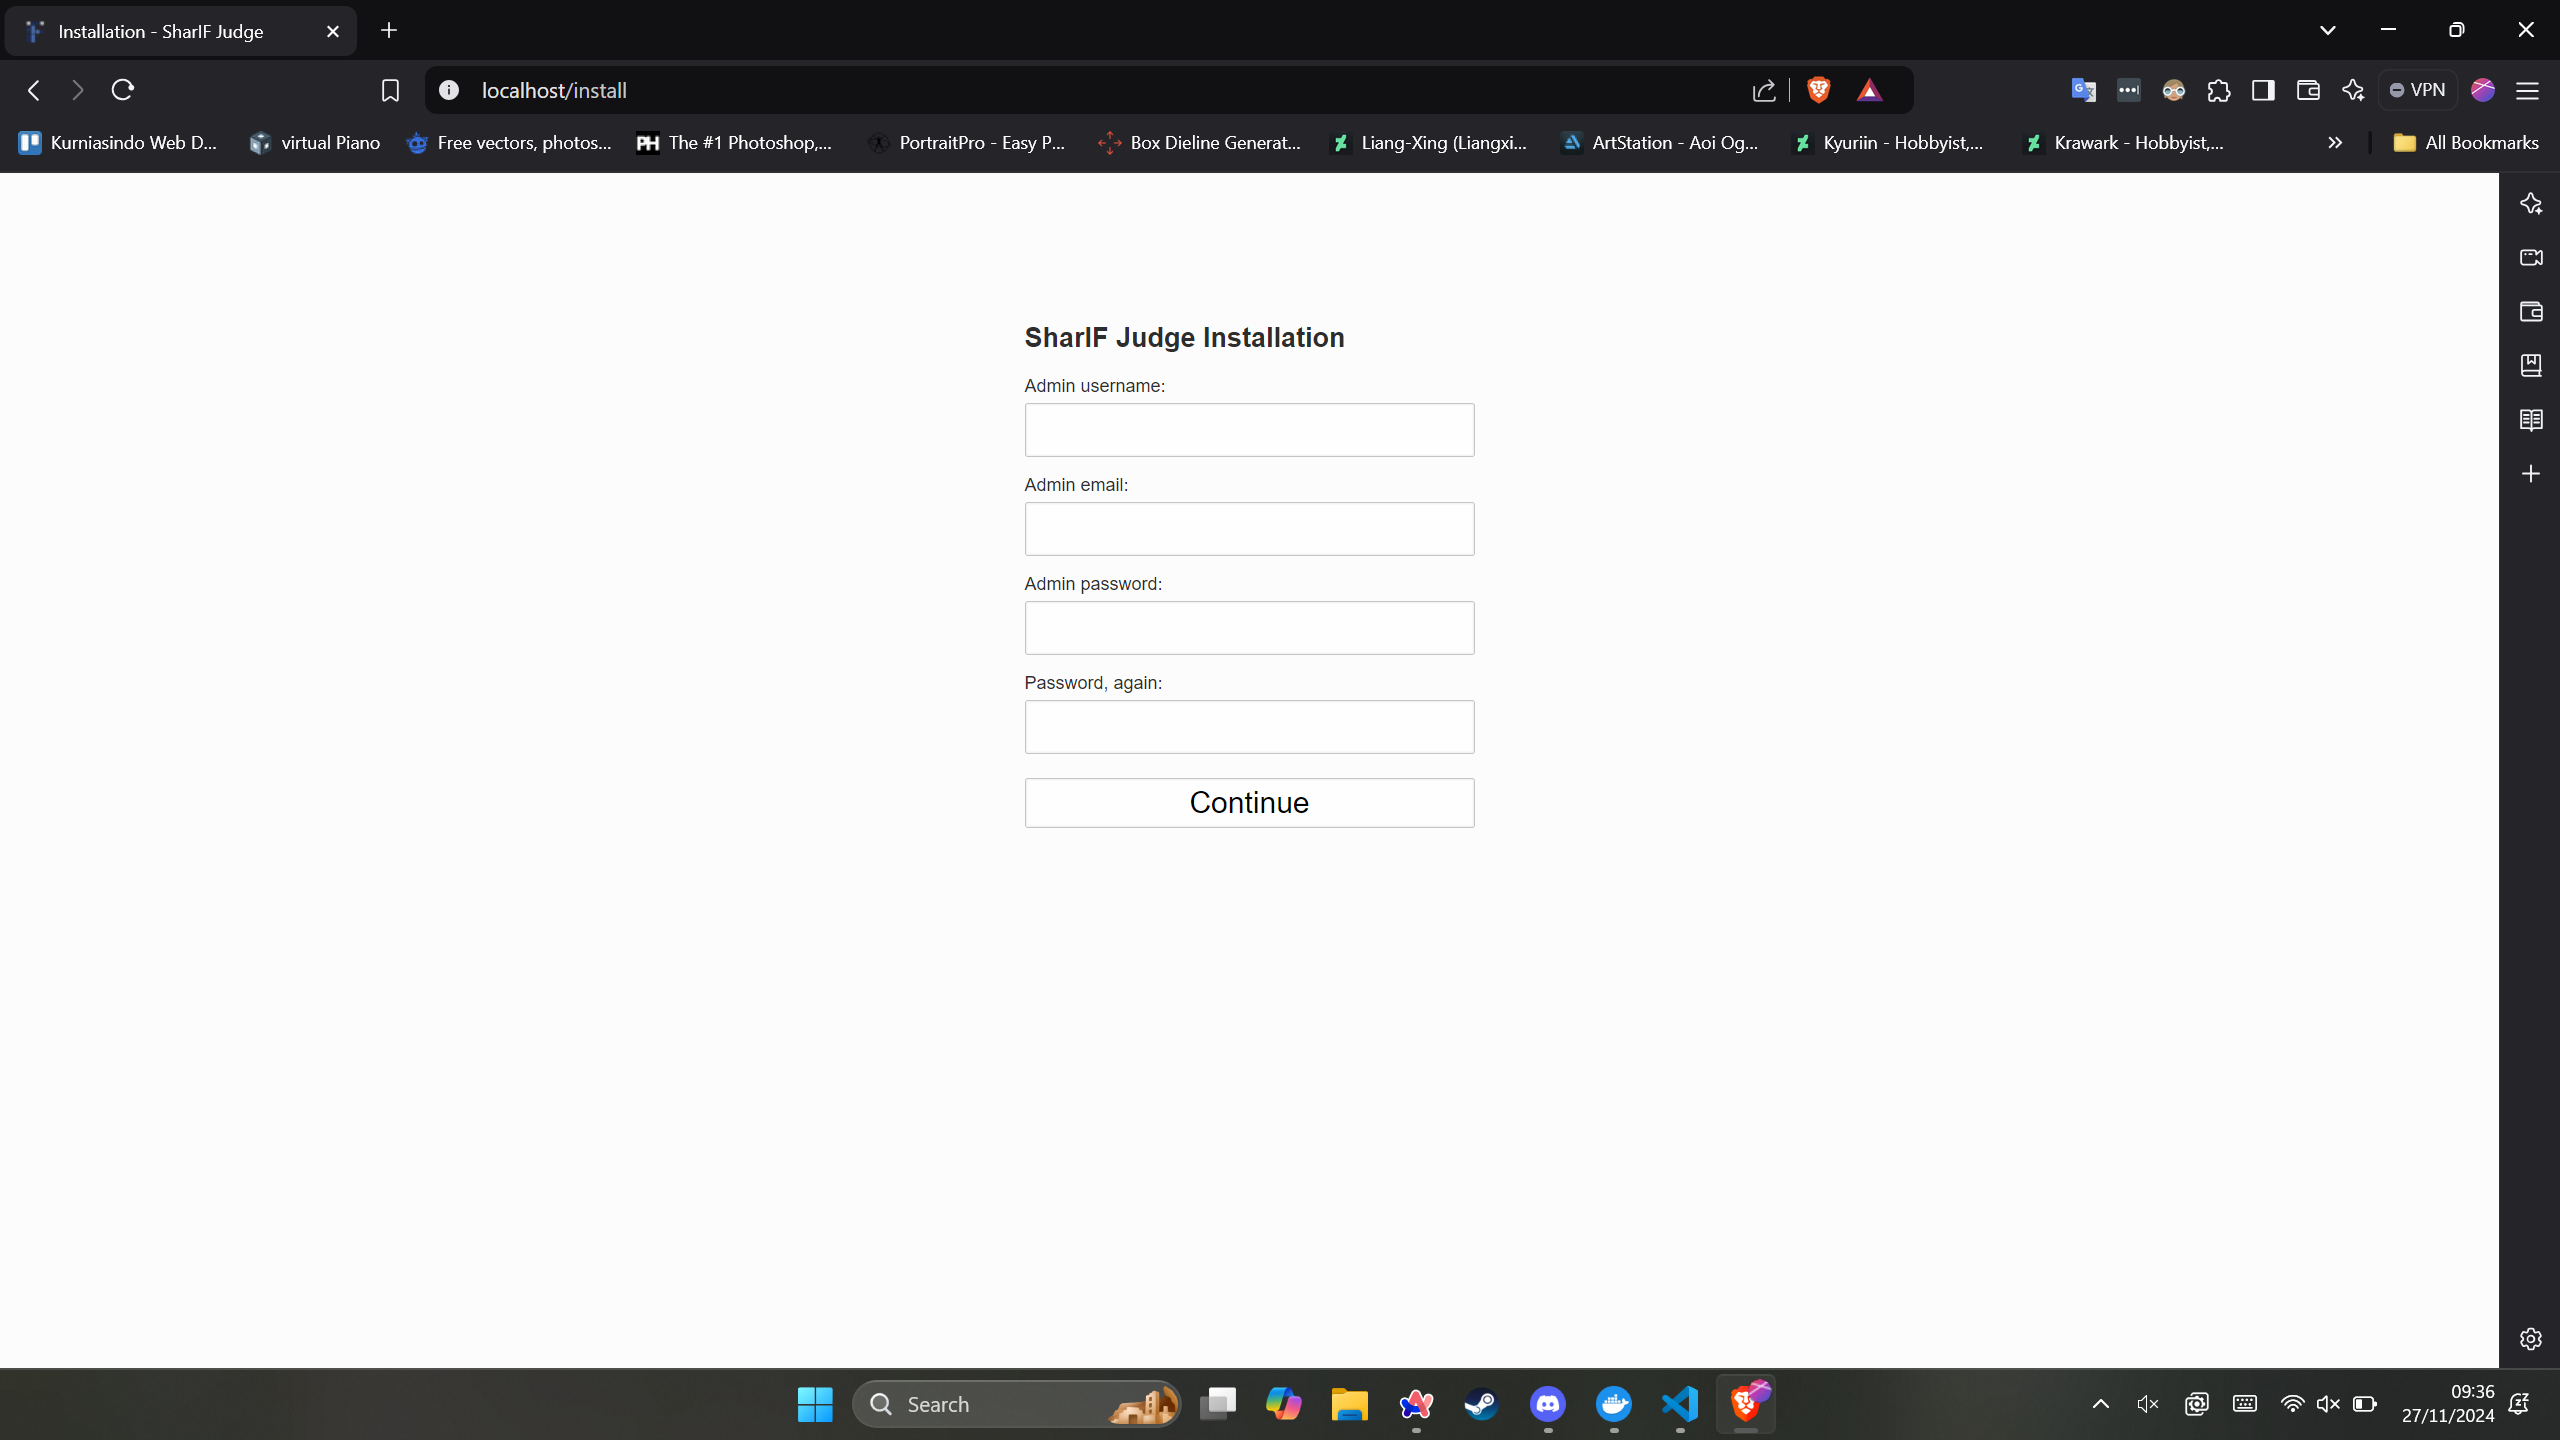
\includegraphics[width=0.85\textwidth]{views/install.png}
				                  \caption{Halaman Install}
				                  \label{fig:3:1:1:install}
			                  \end{figure}


			            \item \verb|Login.php| \\
			                  Berikut fungsi dengan penjelasannya pada \textit{controller} \verb|Login.php|:

			                  \begin{itemize}
				                  \item \verb|index()| \\
				                        Mengembalikan \textit{view} \verb|login.twig| dan memeriksa username dan password pada \textit{form} saat di kirim. Gambar \ref{fig:3:1:1:login} menunjukkan hasil halaman Login.

				                        \begin{figure}[H]
					                        \centering
					                        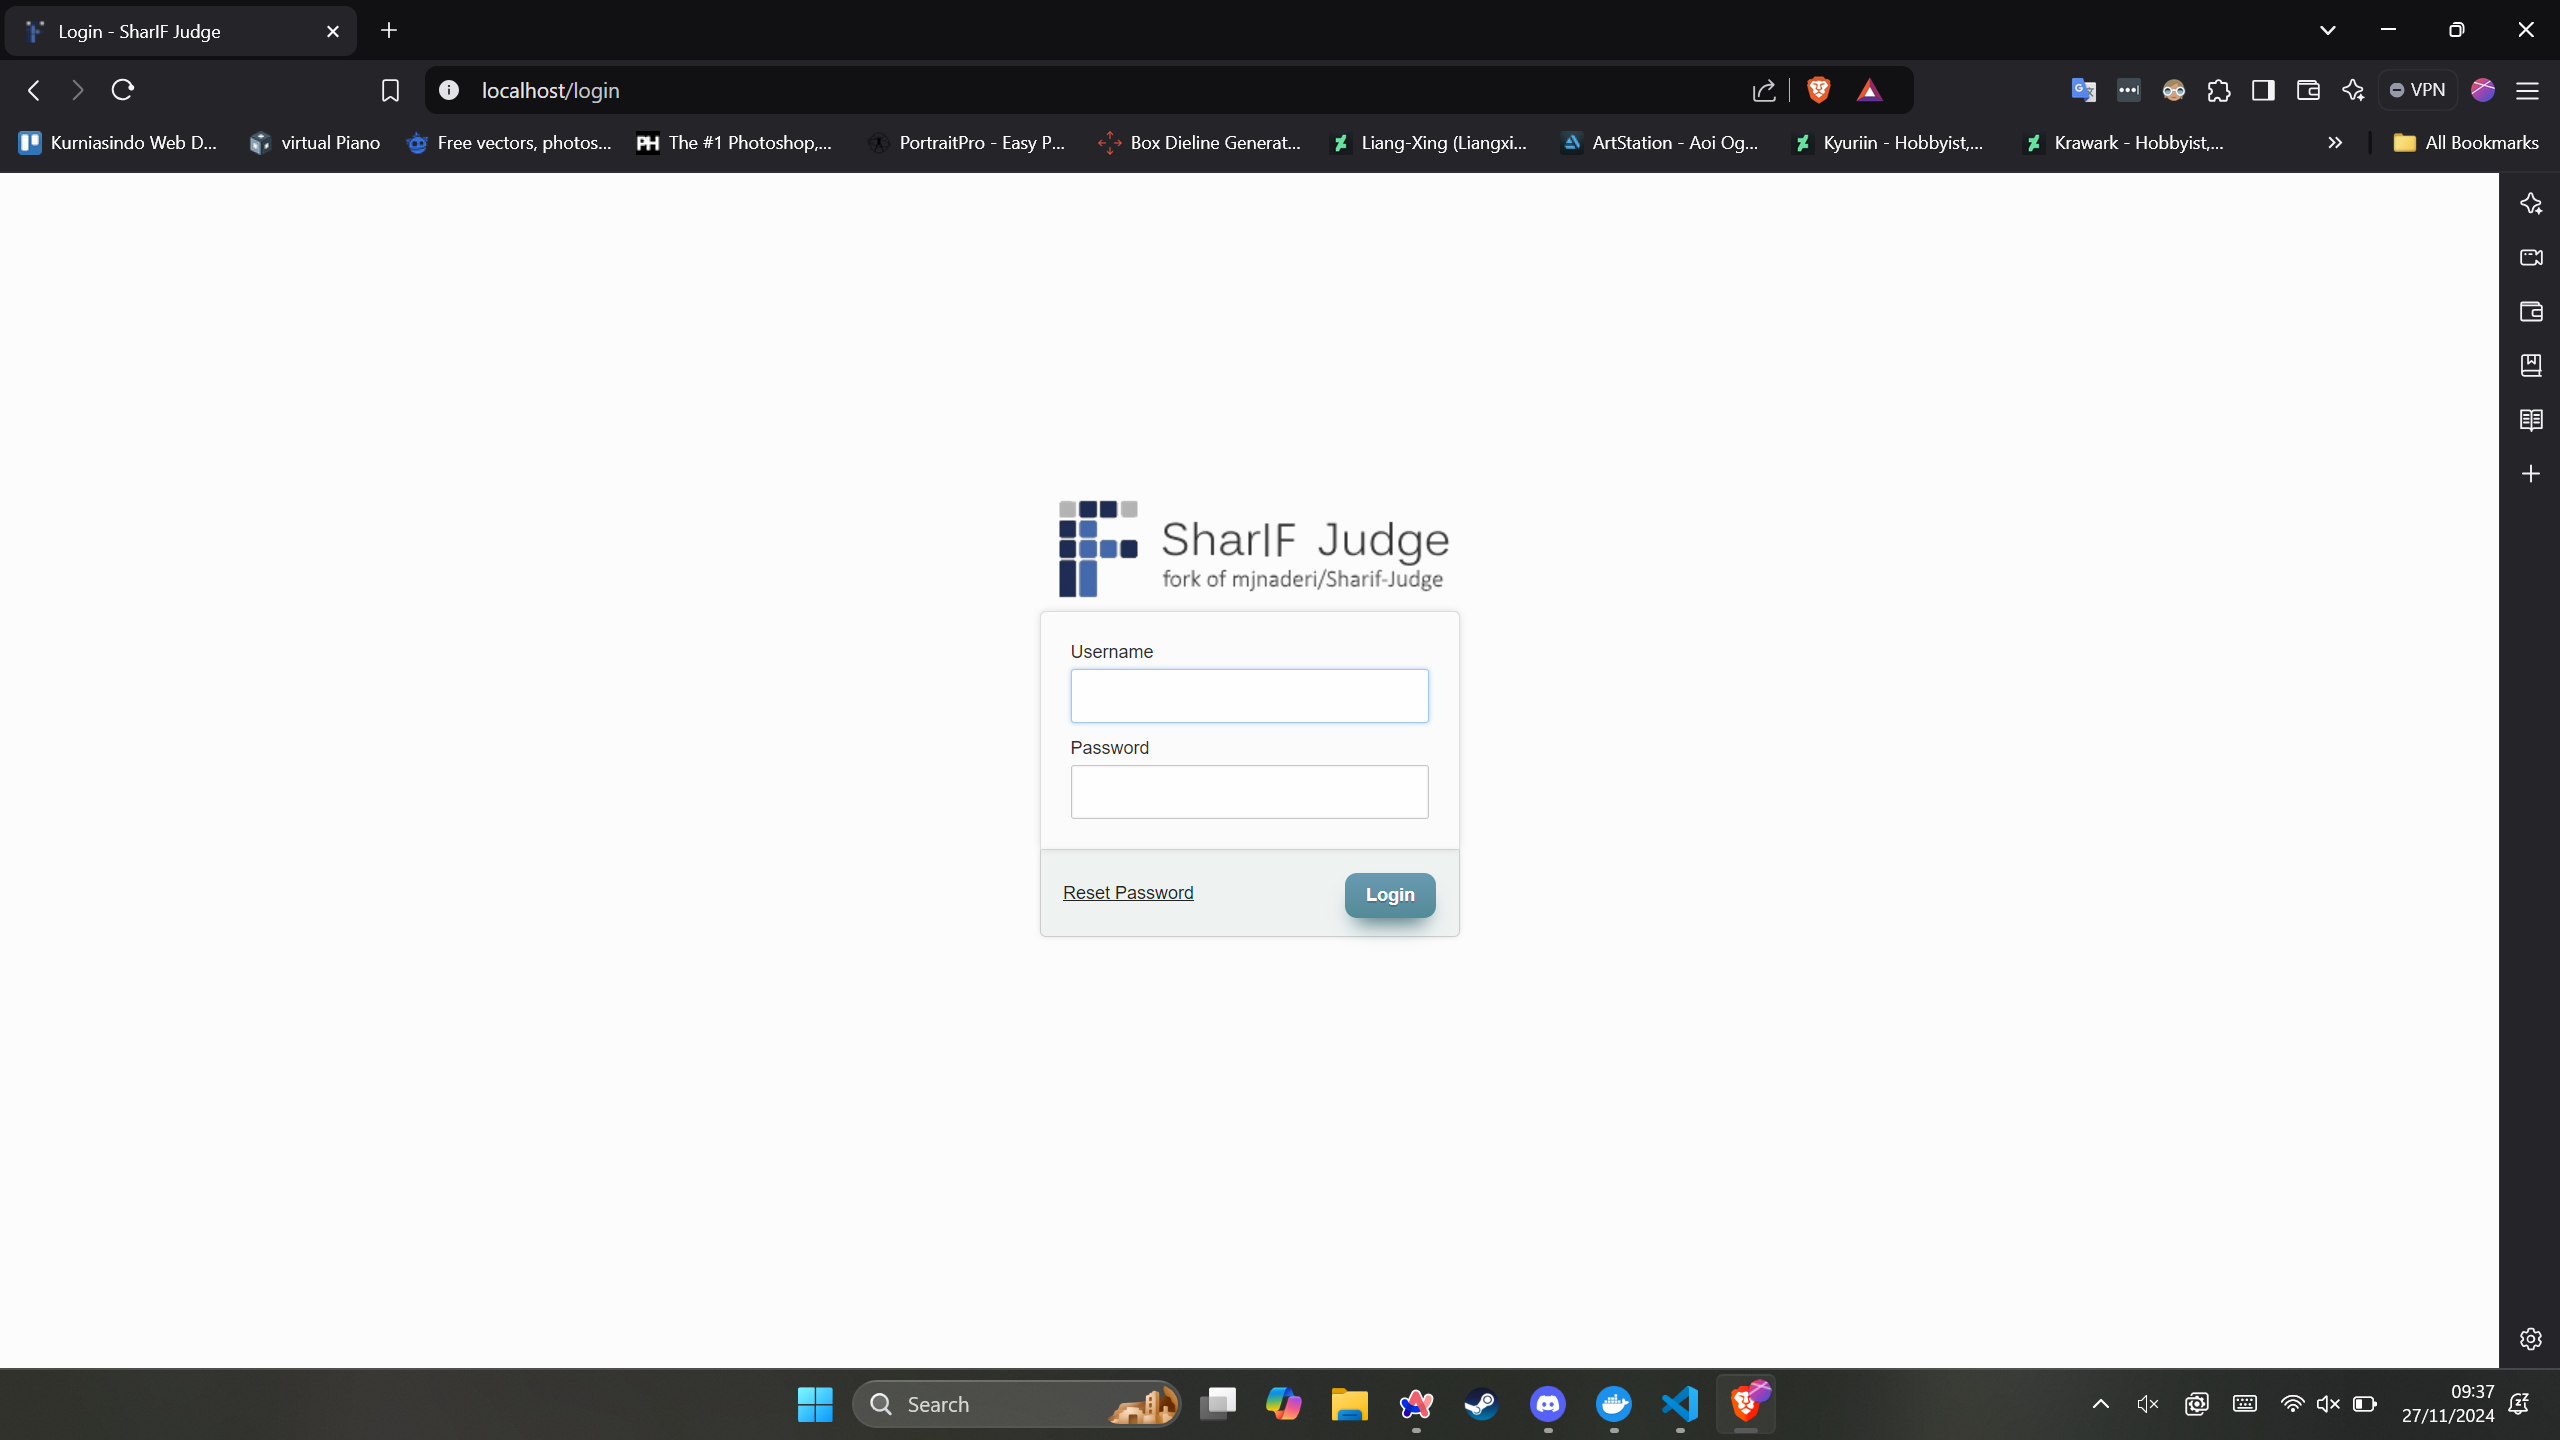
\includegraphics[width=0.85\textwidth]{views/login.png}
					                        \caption{Halaman Login}
					                        \label{fig:3:1:1:login}
				                        \end{figure}
				                  \item \verb|_registration_code($code)| \\
				                        Melakukan validasi kode registrasi.
				                  \item \verb|register()| \\
				                        Menunjukkan halaman \verb|register.twig| dan membuat \textit{user} baru.
				                  \item \verb|logout()| \\
				                        Melakukan \textit{Log out} dan mengalihkan ke halaman \textit{login}.
				                  \item \verb|lost()| \\
				                        Mengirimkan email \textit{reset password}.
				                  \item \verb|reset($passchange_key)| \\
				                        Melakukan \textit{reset password} dengan halaman \verb|reset_password.twig|.

			                  \end{itemize}

			            \item \verb|Logs.php| \\
			                  Pada \textit{controller} \verb|Logs.php| hanya memiliki satu fungsi yaitu \verb|index()|, dimana fungsi tersebut akan mendapatkan data dari \verb|Logs_model| dan memunculkan halaman \verb|logs.twig|. Gambar \ref{fig:3:1:1:log} menunjukkan halaman Log yang dinamakan halaman 24-Hour Log.

			                  \begin{figure}[H]
				                  \centering
				                  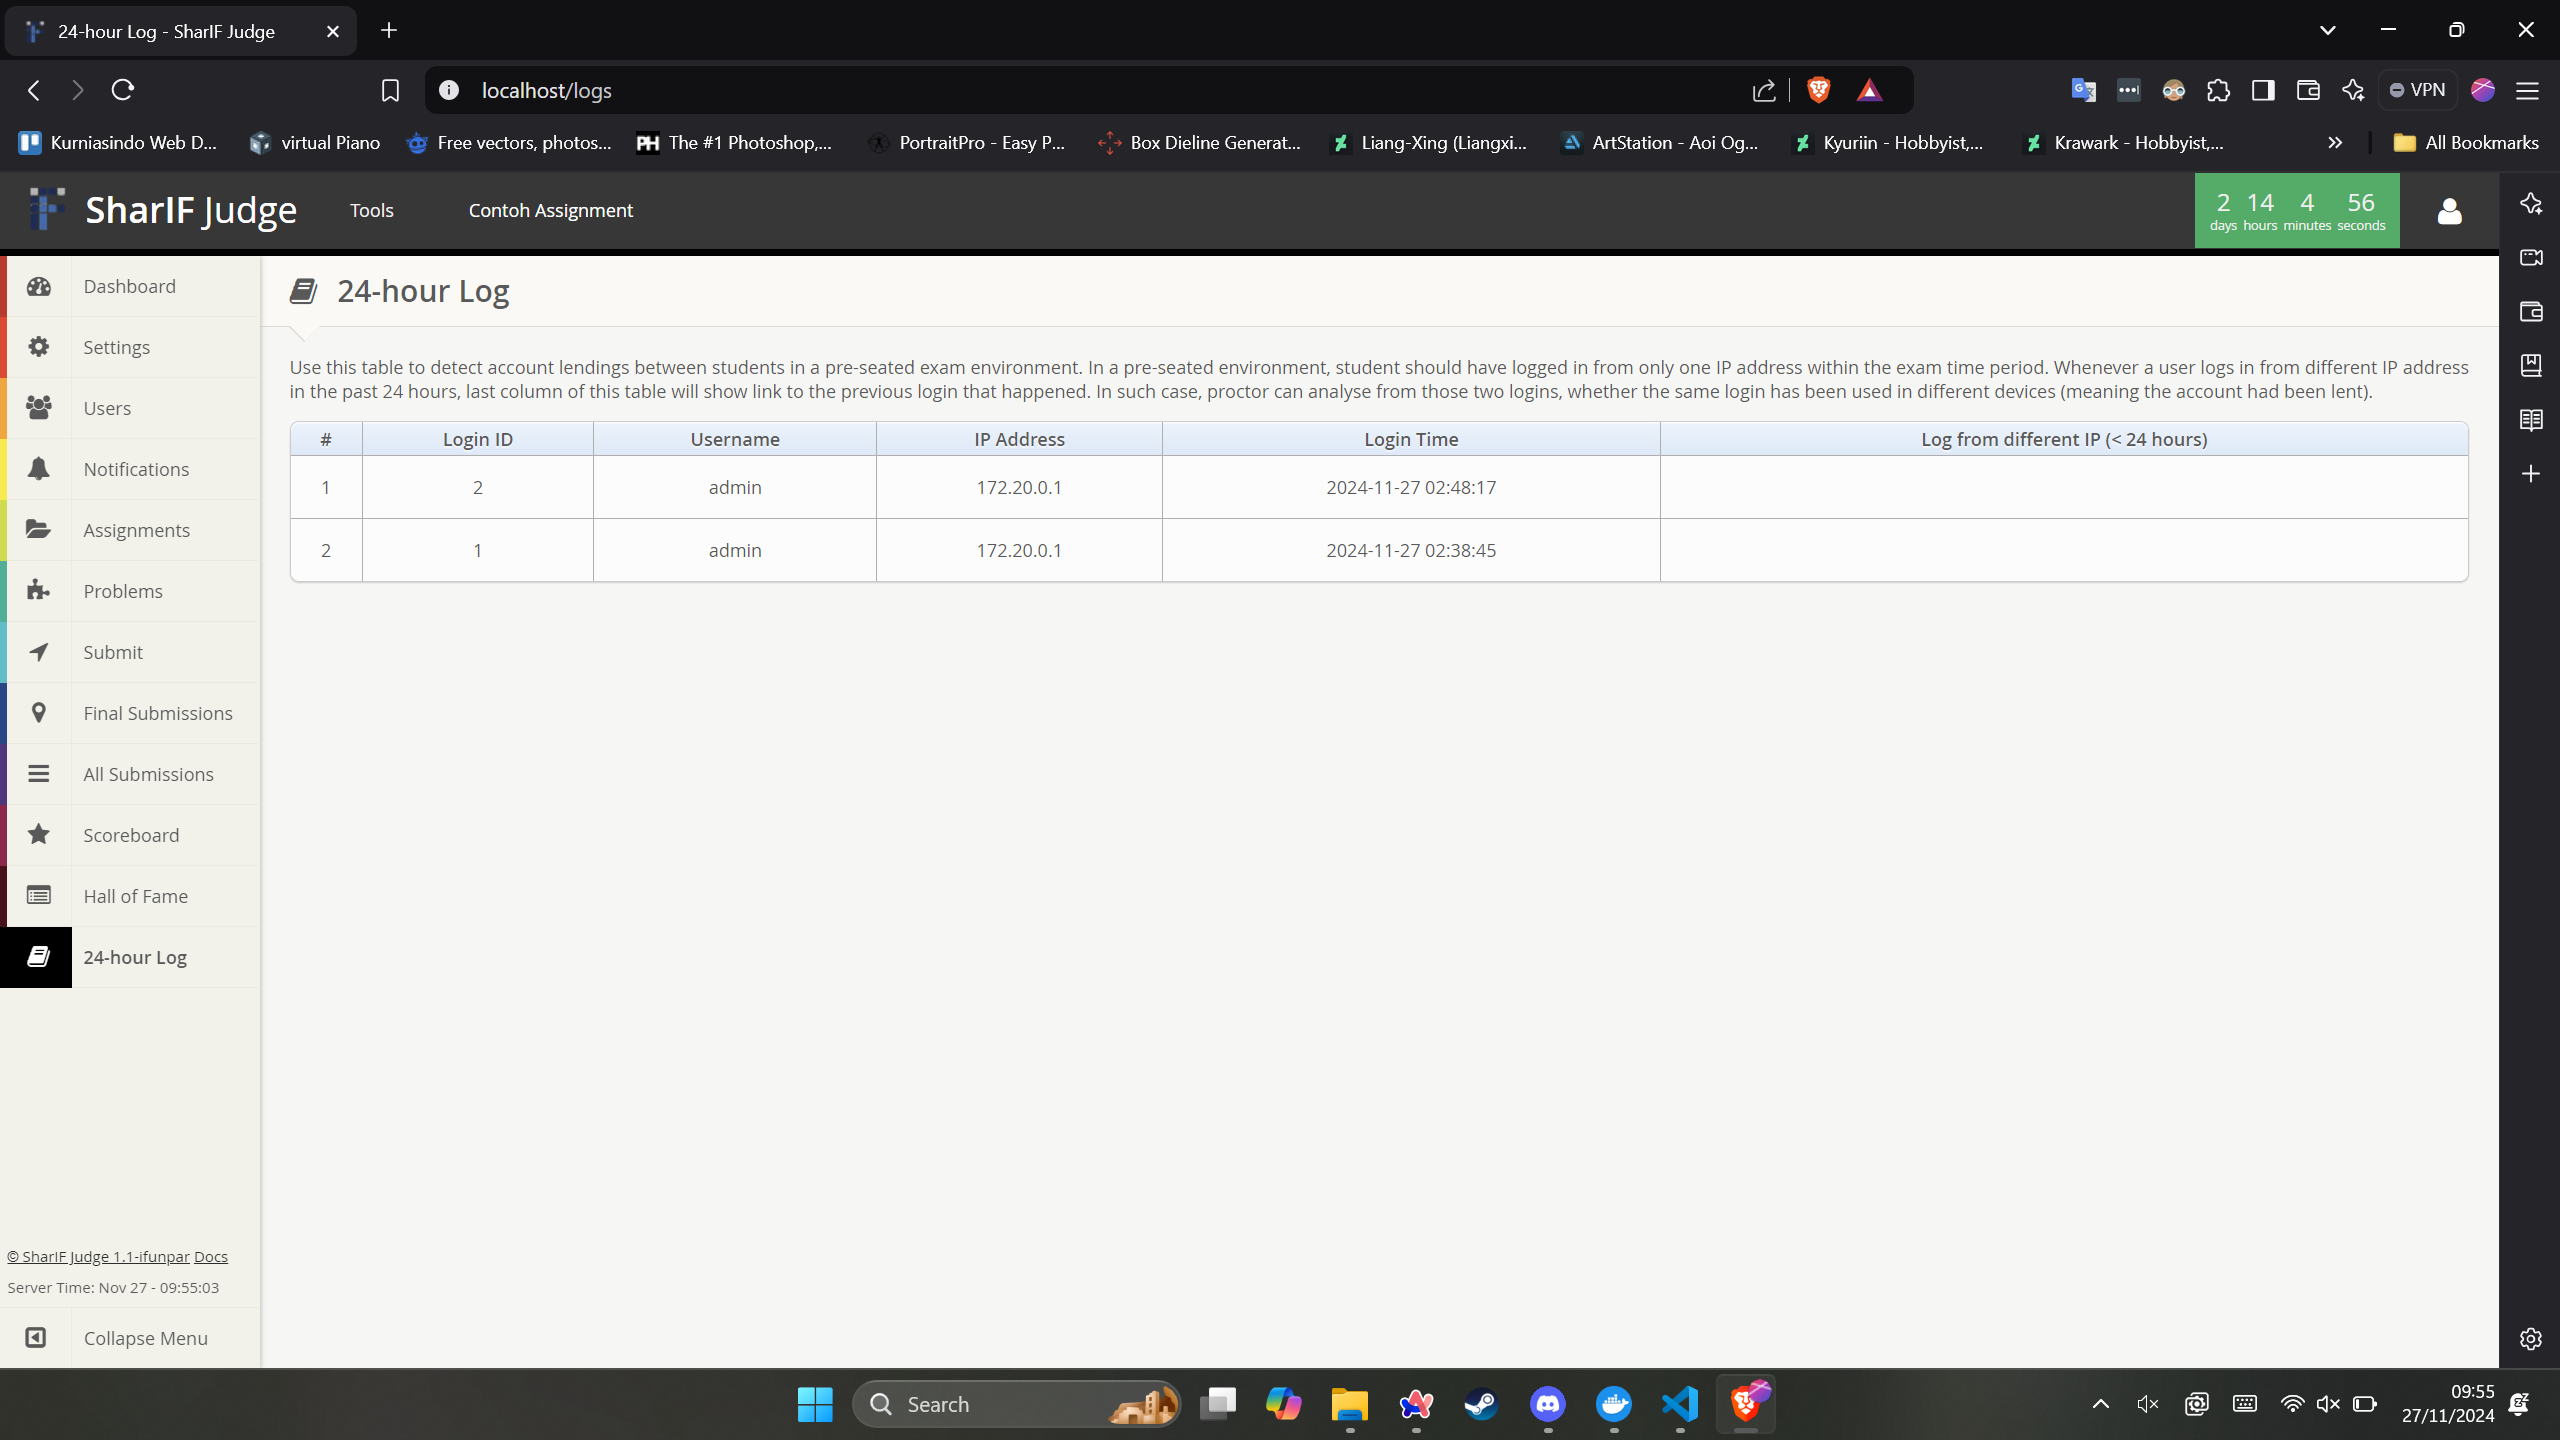
\includegraphics[width=\textwidth]{views/log.png}
				                  \caption{Halaman 24-Hour Log}
				                  \label{fig:3:1:1:log}
			                  \end{figure}


			            \item \verb|Moss.php| \\
			                  Berikut fungsi dengan penjelasannya pada \textit{controller} \verb|Moss.php|:

			                  \begin{itemize}
				                  \item \verb|update($assignment_id)| \\
				                        Memperbaharui \textit{settings} dari masukkan \verb|moss_userid| pengguna.
				                  \item \verb|_detect($assignment_id)| \\
				                        Melakukan pemeriksaan kesamaan kode dengan Moss.
				                  \item \verb|index()| \\
				                        Mengambil data dan memasukkannya ke dalam \textit{view} \verb|moss.twig|. Gambar \ref{fig:3:1:1:moss} merupakan hasil halaman moss. Fungsi \verb|_detect| juga akan dijalankan saat \textit{form} terkirim.

				                        \begin{figure}[H]
					                        \centering
					                        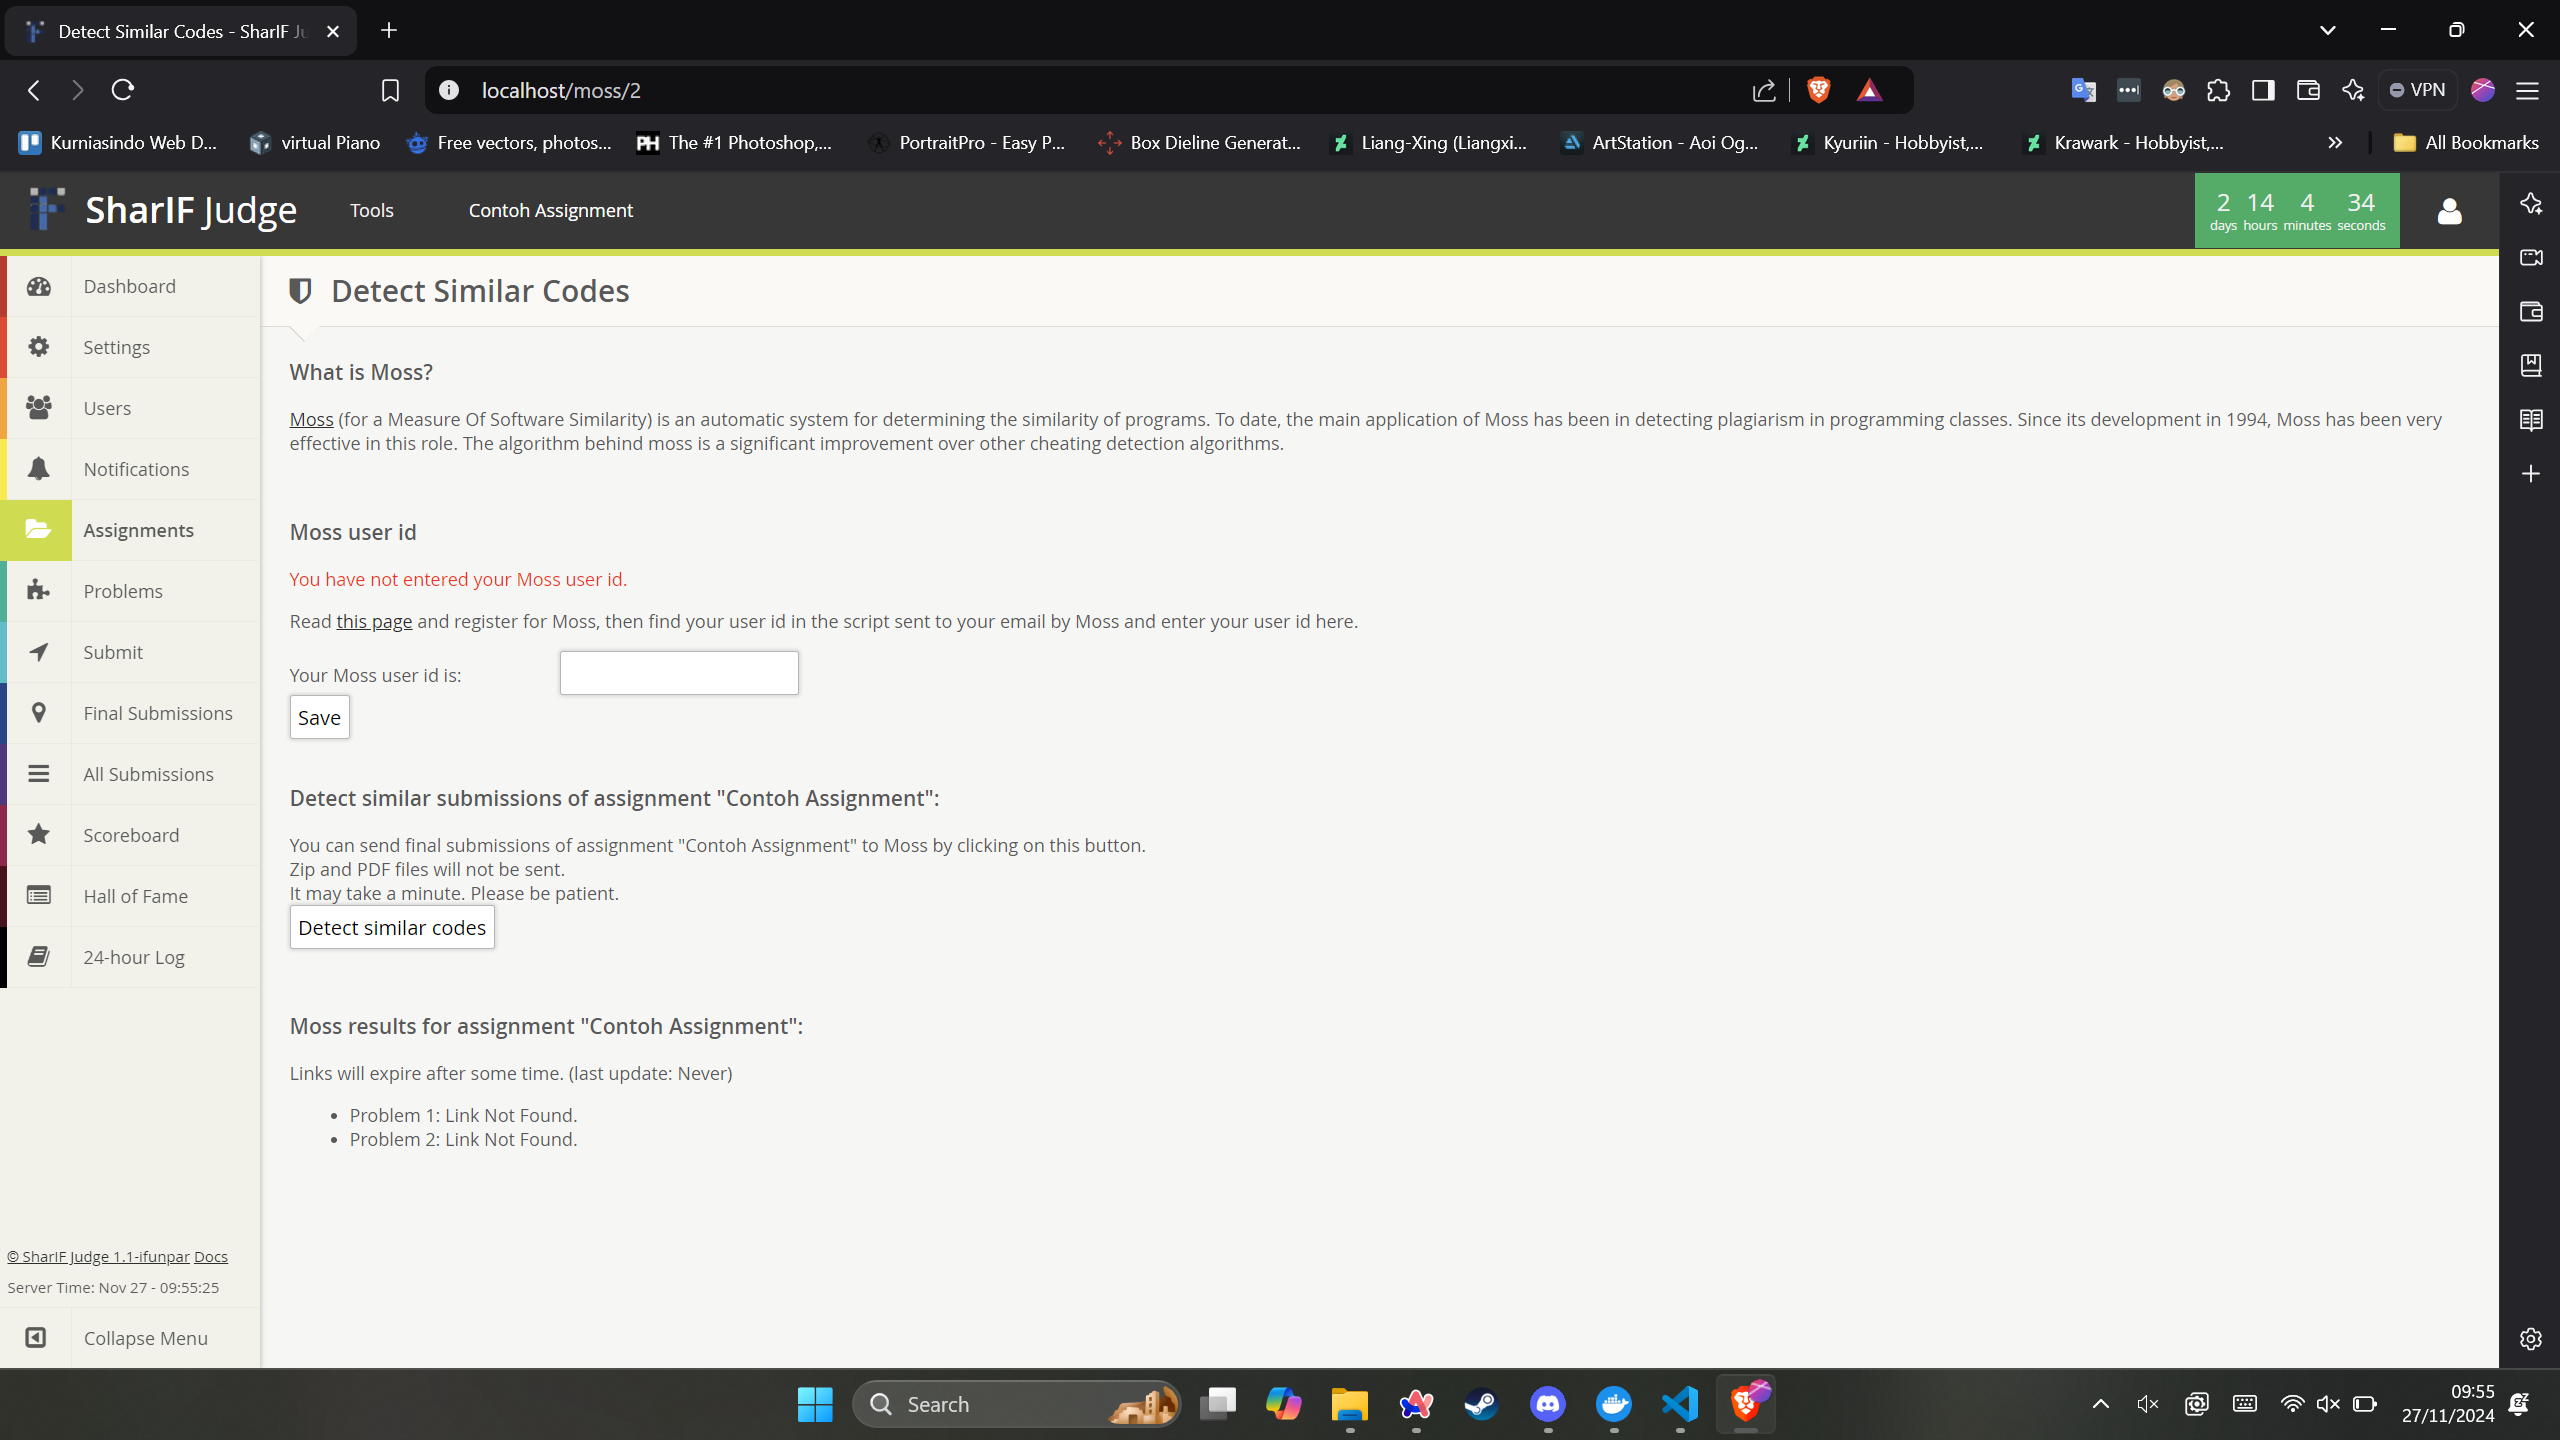
\includegraphics[width=0.8\textwidth]{views/moss.png}
					                        \caption{Halaman Moss}
					                        \label{fig:3:1:1:moss}
				                        \end{figure}

			                  \end{itemize}

			            \item \verb|Notifications.php| \\
			                  Berikut fungsi dengan penjelasannya pada \textit{controller} \verb|Notifications.php|:

			                  \begin{itemize}
				                  \item \verb|add()| \\
				                        Menambahkan atau memperbaharui sebuah \textit{notification}.
				                  \item \verb|edit($notif_id)| \\
				                        Menandai \textit{notification} yang akan di \textit{edit} dan memanggil fungsi \verb|add|.
				                  \item \verb|delete()| \\
				                        Menghapus sebuah \textit{notification}.
				                  \item \verb|check()| \\
				                        Mengunakan \textit{ajax request} untuk mengetahui ketersediaan \textit{notification} baru.
				                  \item \verb|index()| \\
				                        Mendapatkan data dari dua model yaitu \verb|Assignment_model| dan \verb|Notifications_model|. Data akan dimasukkan ke dalam \textit{view} \verb|notifications.twig| yang akan dikembalikan ke pengguna. Gambar \ref{fig:3:1:1:notif} menunjukkan hasil halaman \textit{Notifications}.

				                        \begin{figure}[H]
					                        \centering
					                        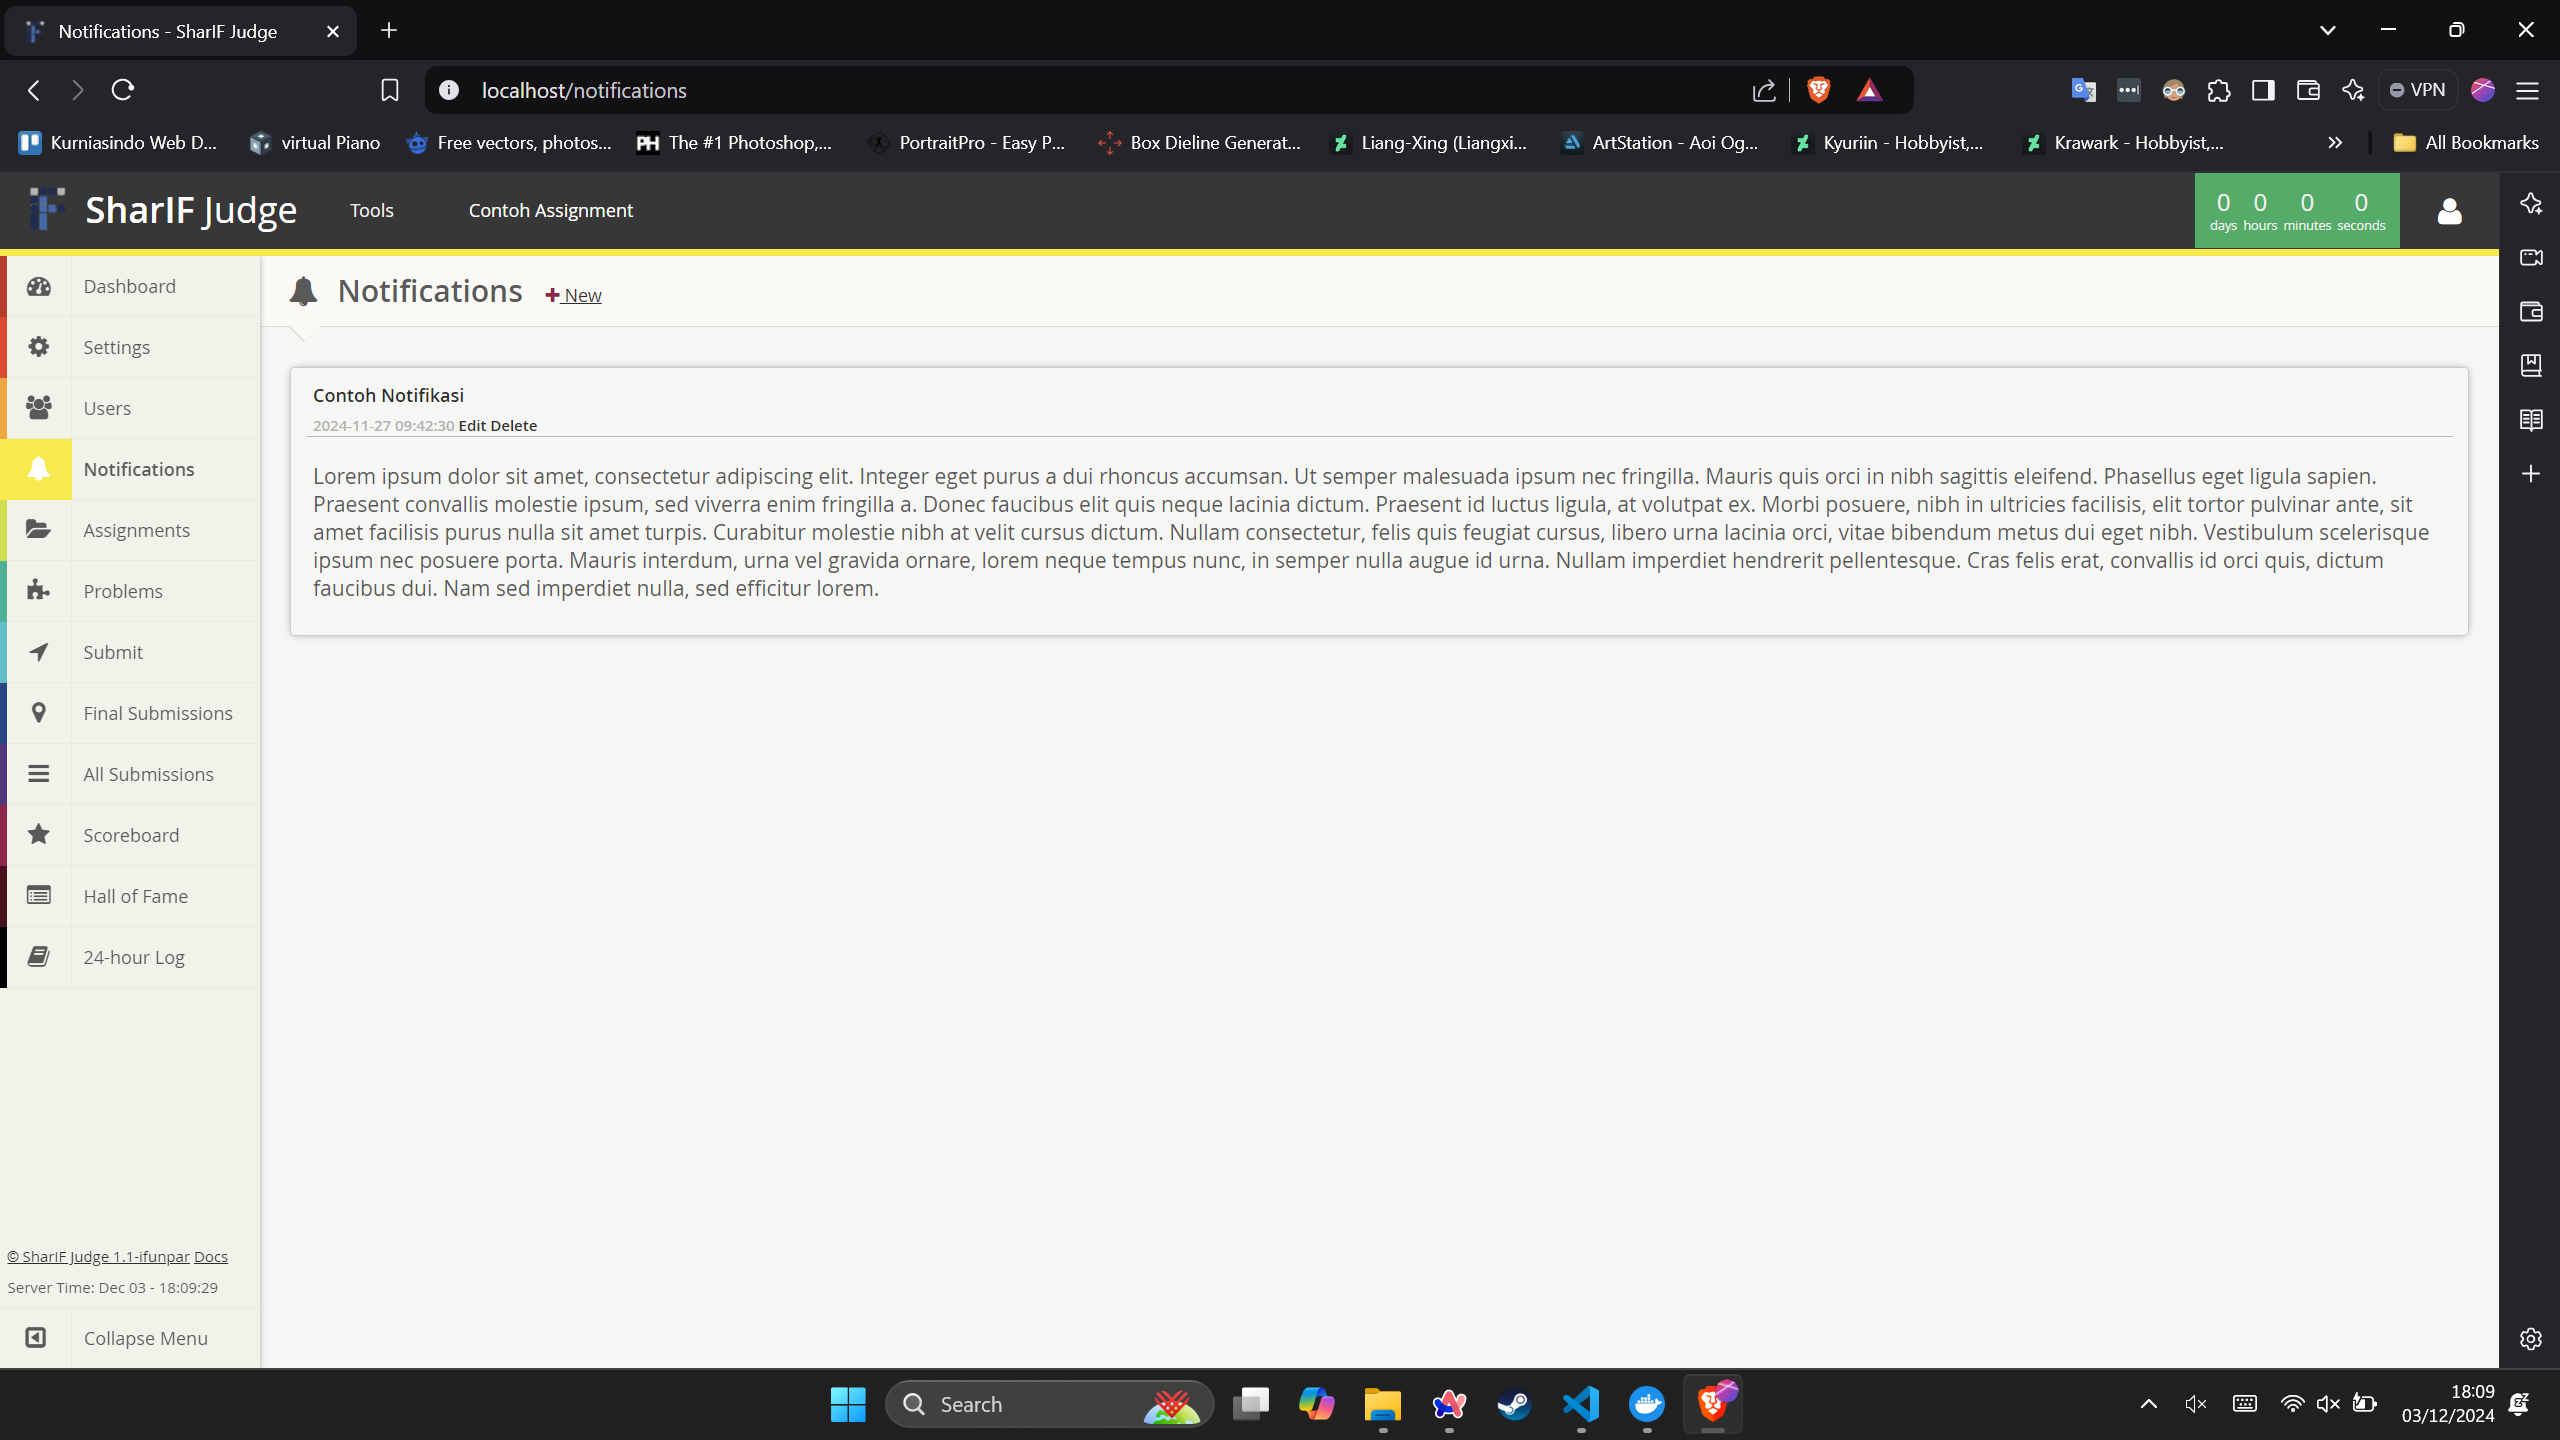
\includegraphics[width=0.8\textwidth]{views/notifications.png}
					                        \caption{Halaman Notifications}
					                        \label{fig:3:1:1:notif}
				                        \end{figure}

			                  \end{itemize}

			            \item \verb|Problems.php| \\
			                  Berikut fungsi dengan penjelasannya pada \textit{controller} \verb|Notifications.php|:

			                  \begin{itemize}
				                  \item \verb|edit()| \\
				                        Memperbaharui deskripsi sebuah \textit{problem} dalam bentuk \verb|html| atau \verb|markdown|.
				                  \item \verb|index()| \\
				                        Mendapatkan data \textit{problem} dari berbagai \textit{model} sesuai dengan \textit{assignment} yang dipilih dan menaruh data tersebut pada halaman \verb|problems.twig| yang akan ditampilkan ke pengguna. Gambar \ref{fig:3:1:1:problem} menunjukkan hasil halaman Problems.

				                        \begin{figure}[H]
					                        \centering
					                        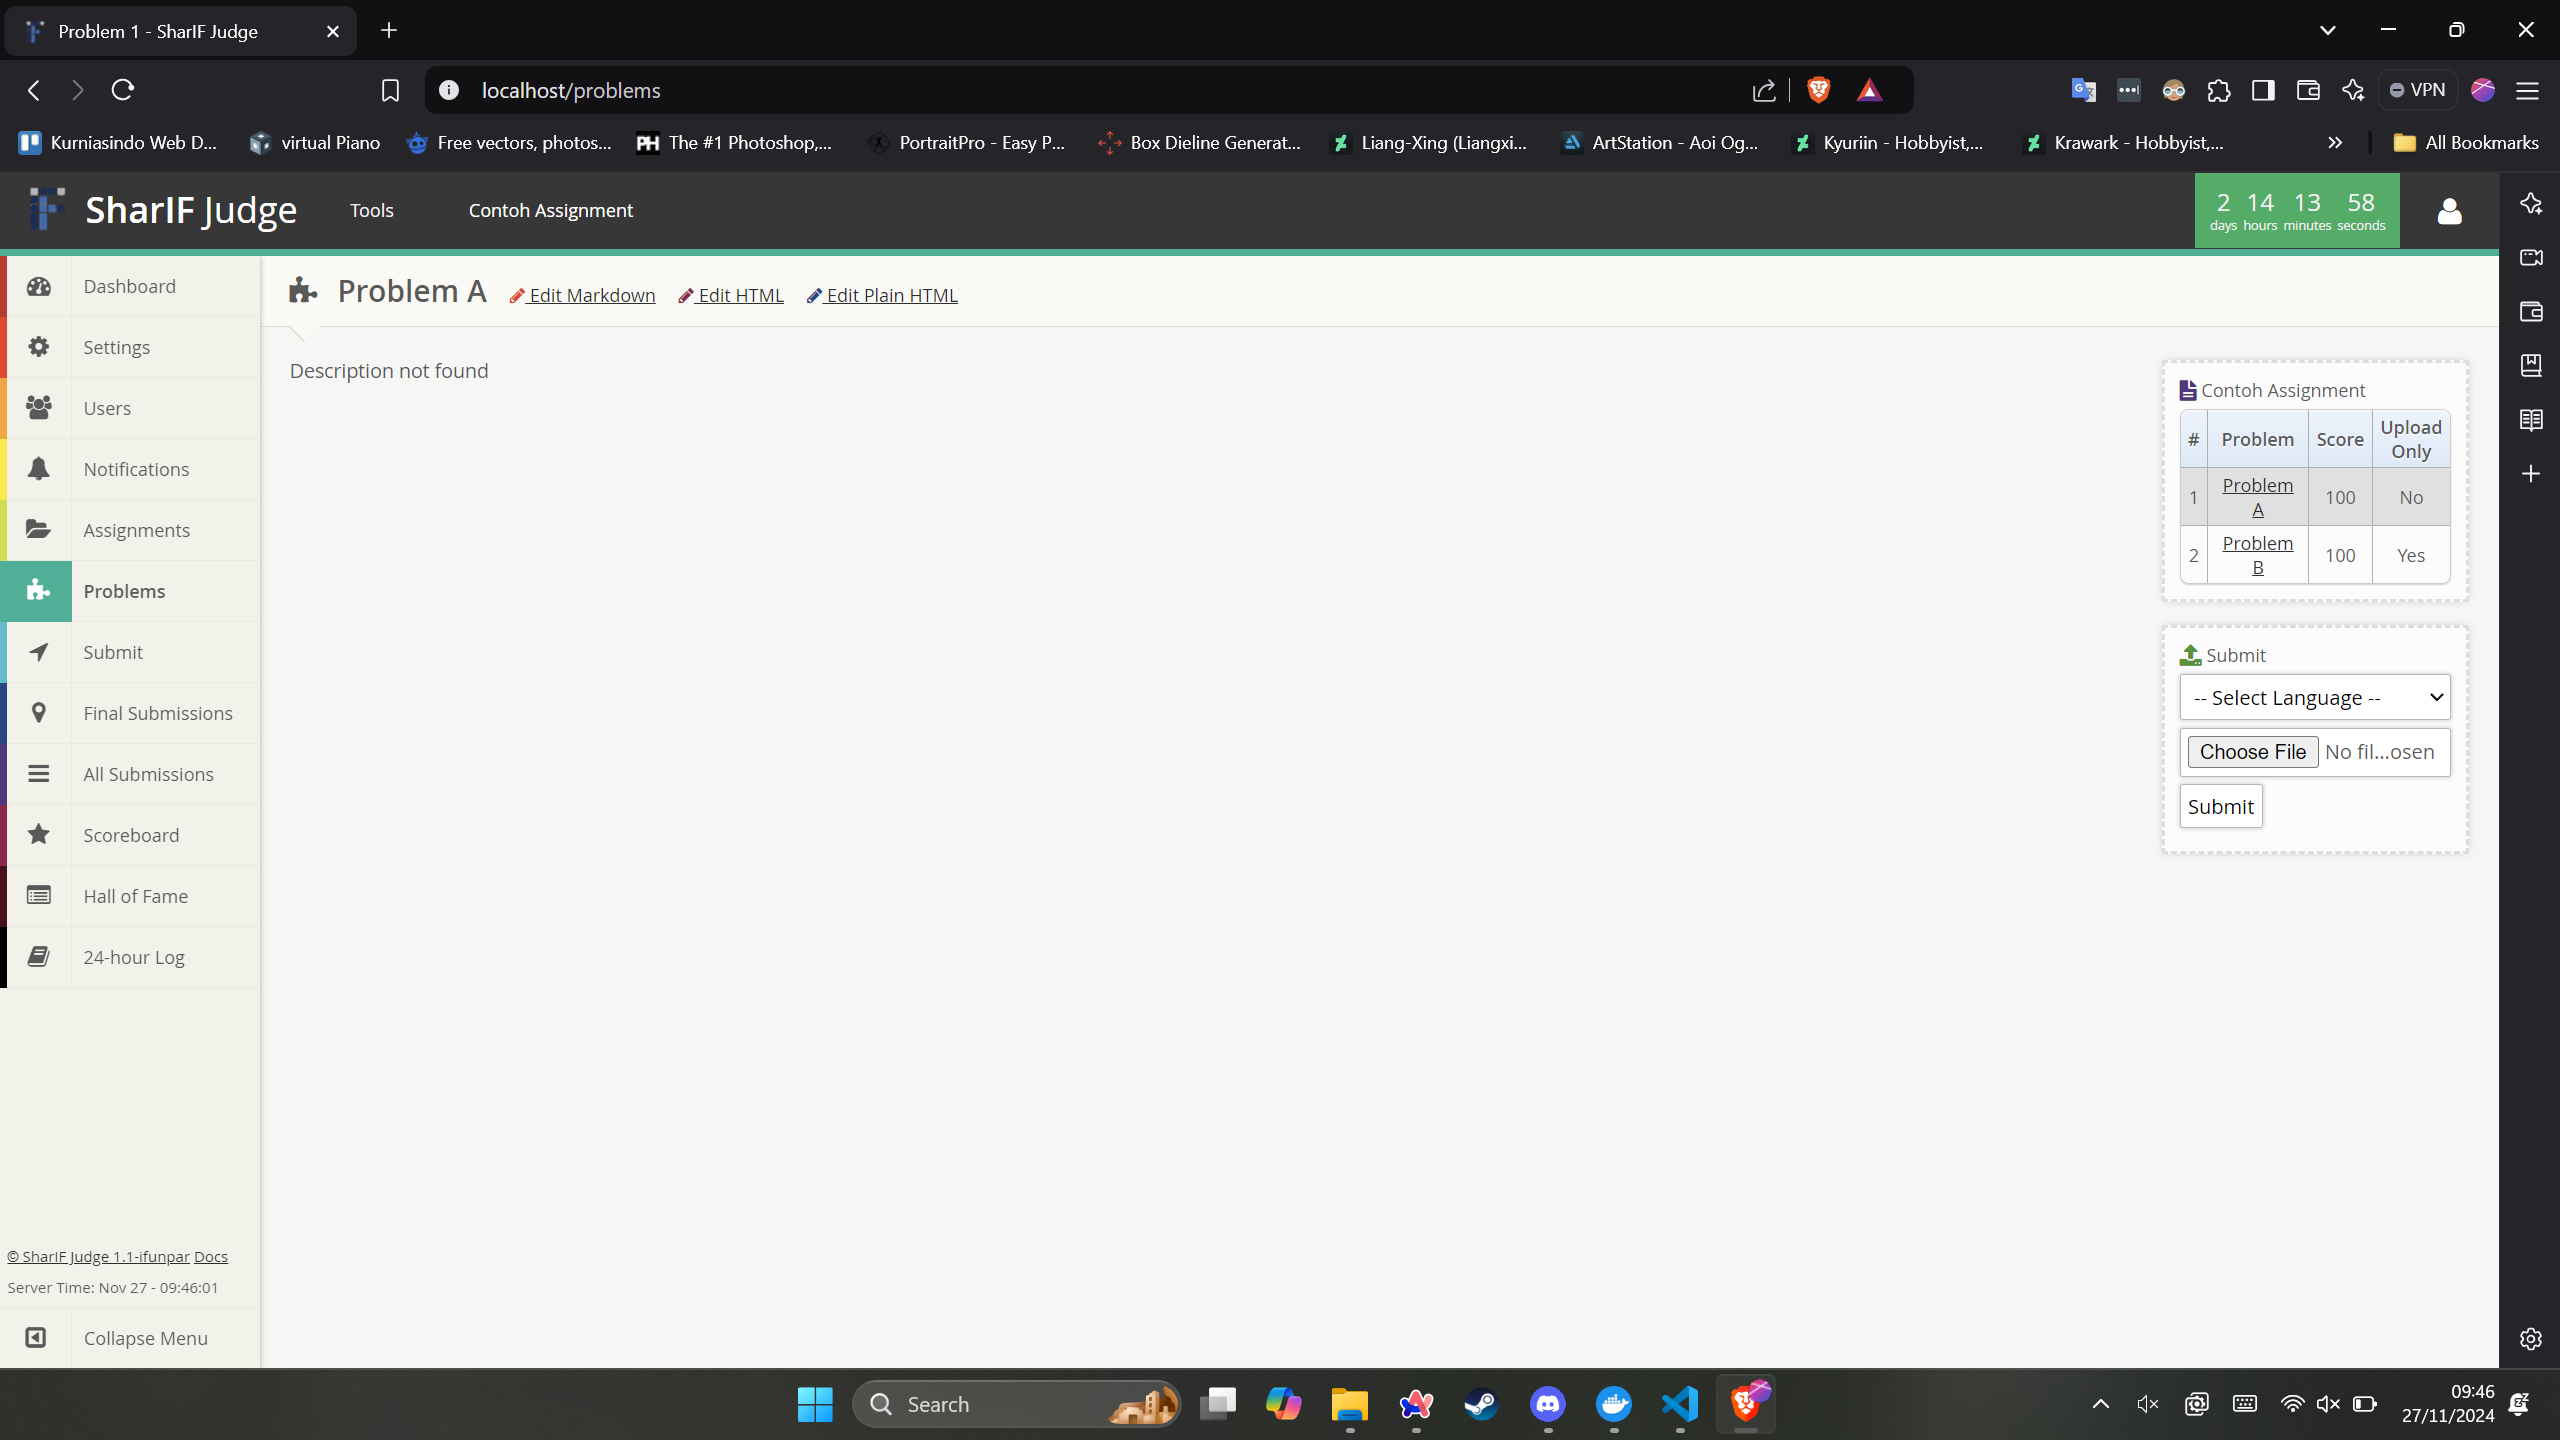
\includegraphics[width=0.8\textwidth]{views/problem.png}
					                        \caption{Halaman Problems}
					                        \label{fig:3:1:1:problem}
				                        \end{figure}

			                  \end{itemize}

			            \item \verb|Profile.php| \\
			                  Berikut fungsi dengan penjelasannya pada \textit{controller} \verb|Profile.php|:

			                  \begin{itemize}
				                  \item \verb|index()| \\
				                        Mendapatkan data dari berbagai \textit{model} terutama dari \textit{User} yang akan dimasukkan ke dalam \textit{view} \verb|profile.twig|. Fungsi ini juga menangani pengiriman \textit{form} pembaharuan data \textit{user} pengguna. Gambar \ref{fig:3:1:1:profile} menunjukkan hasil halaman Profile.

				                        \begin{figure}[H]
					                        \centering
					                        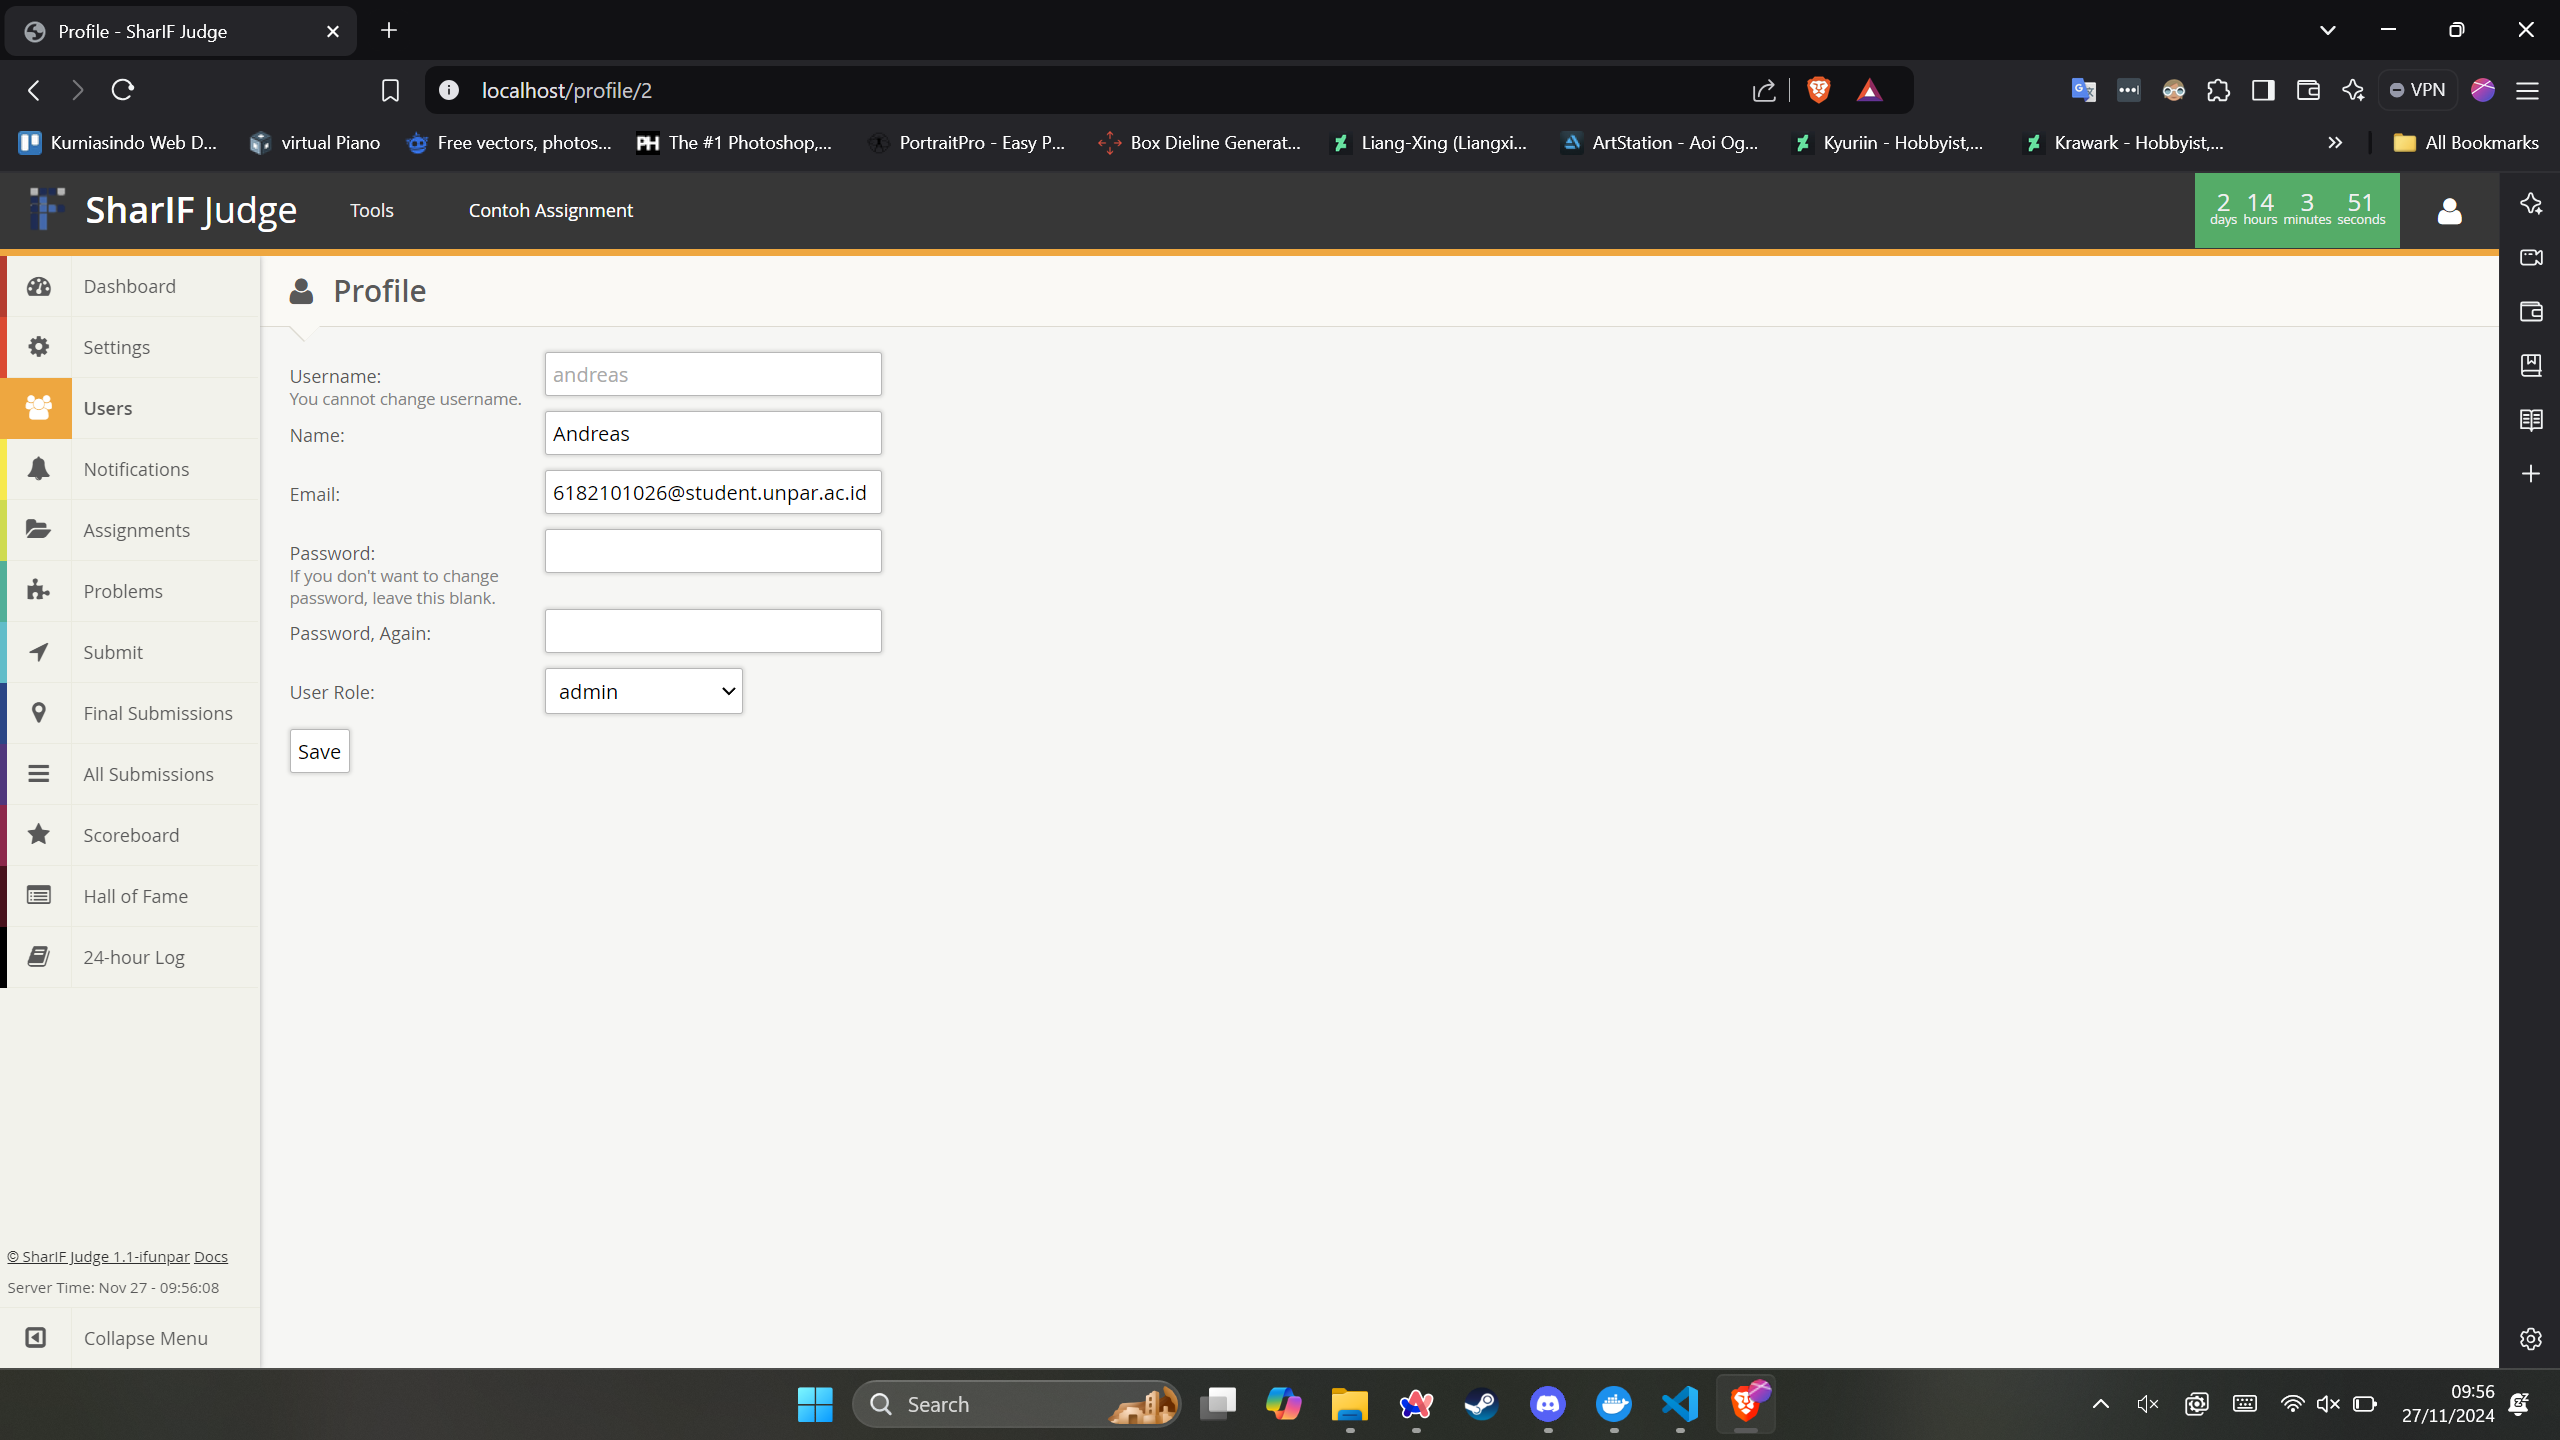
\includegraphics[width=0.8\textwidth]{views/profile.png}
					                        \caption{Halaman Profile}
					                        \label{fig:3:1:1:profile}
				                        \end{figure}
				                  \item \verb|_password_check($str)| \\
				                        Melakukan validasi \textit{input password}.
				                  \item \verb|_password_again_check($str)| \\
				                        Melakukan validasi \textit{input} tulisan pengulangan \textit{password}.
				                  \item \verb|_email_check($str)| \\
				                        Melakukan validasi ketersediaan email pada \textit{database}.
				                  \item \verb|_role_check($str)| \\
				                        Melakukan validasi \textit{role} pengguna saat ingin mengubah \textit{role user}.
			                  \end{itemize}

			            \item \verb|Queue.php| \\
			                  Berikut fungsi dengan penjelasannya pada \textit{controller} \verb|Profile.php|:

			                  \begin{itemize}
				                  \item \verb|pause()| \\
				                        Memberhentikan proses \textit{queue}.
				                  \item \verb|resume()| \\
				                        Melanjutkan proses \textit{queue}.
				                  \item \verb|empty_queue()| \\
				                        Menghapus semua \textit{queue} yang ada.
				                  \item \verb|index()| \\
				                        Mendapatkan data dari \textit{model} \verb|Queue|, \verb|Assignments_model|, dan \verb|Settings_model| yang dipakai dalam \textit{view} \verb|queue.twig| dan ditampilkan kepada pengguna. Gambar \ref{fig:3:1:1:queue} menunjukkan hasil halaman Queue.

				                        \begin{figure}[H]
					                        \centering
					                        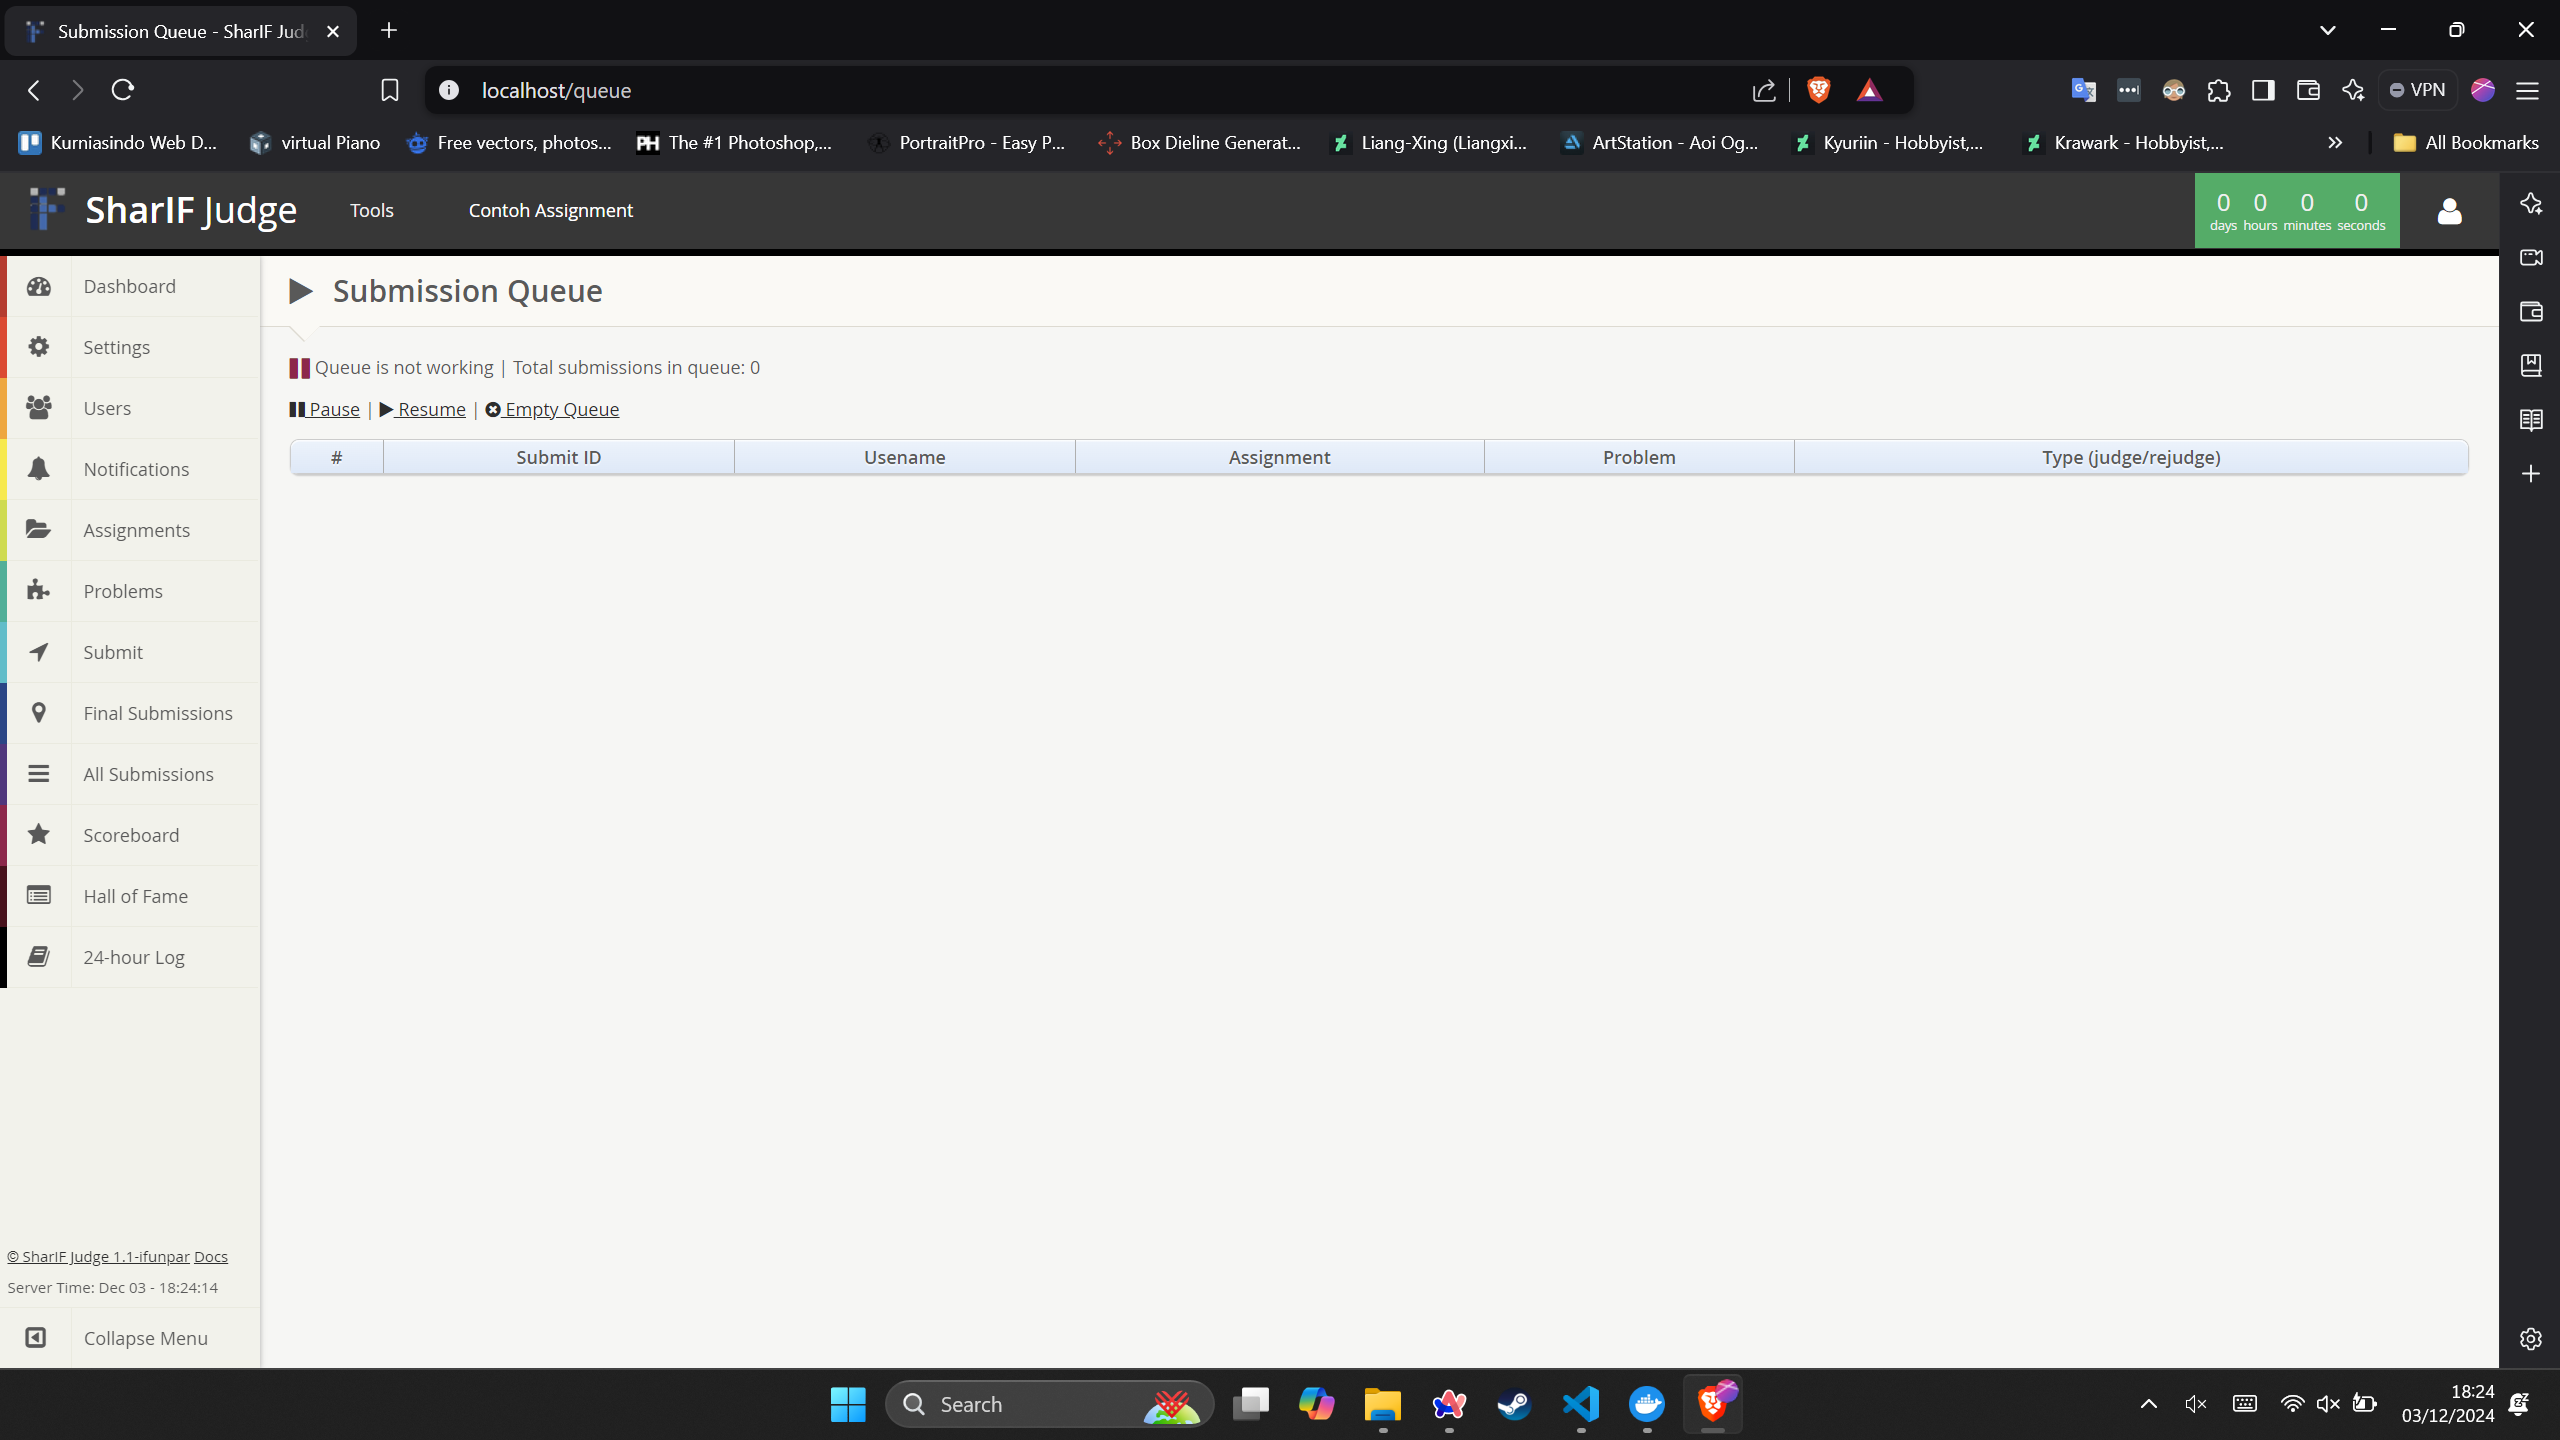
\includegraphics[width=0.8\textwidth]{views/queue.png}
					                        \caption{Halaman Queue}
					                        \label{fig:3:1:1:queue}
				                        \end{figure}

			                  \end{itemize}

			            \item \verb|Queueprocess.php| \\
			                  \textit{Controller} \verb|Queueprocess.php| hanya memiliki satu fungsi yaitu \verb|run()| yang akan menjalankan \textit{queue} satu per satu menggunakan \verb|bash|.

			            \item \verb|Rejudge.php| \\
			                  Berikut fungsi dengan penjelasannya pada \textit{controller} \verb|Profile.php|:

			                  \begin{itemize}
				                  \item \verb|rejudge_single()| \\
				                        Melakukan \textit{rejudge} untuk satu buah \textit{submission}.
				                  \item \verb|index()| \\
				                        Mendapatkan data dan menampilkan \textit{view} \verb|rejudge.twig|. Fungsi ini juga dapat melakukan \textit{rejudge} pada sebuah \textit{problem} tertentu. Gambar \ref{fig:3:1:1:rejudge} menunjukkan halaman Rejudge.

				                        \begin{figure}[H]
					                        \centering
					                        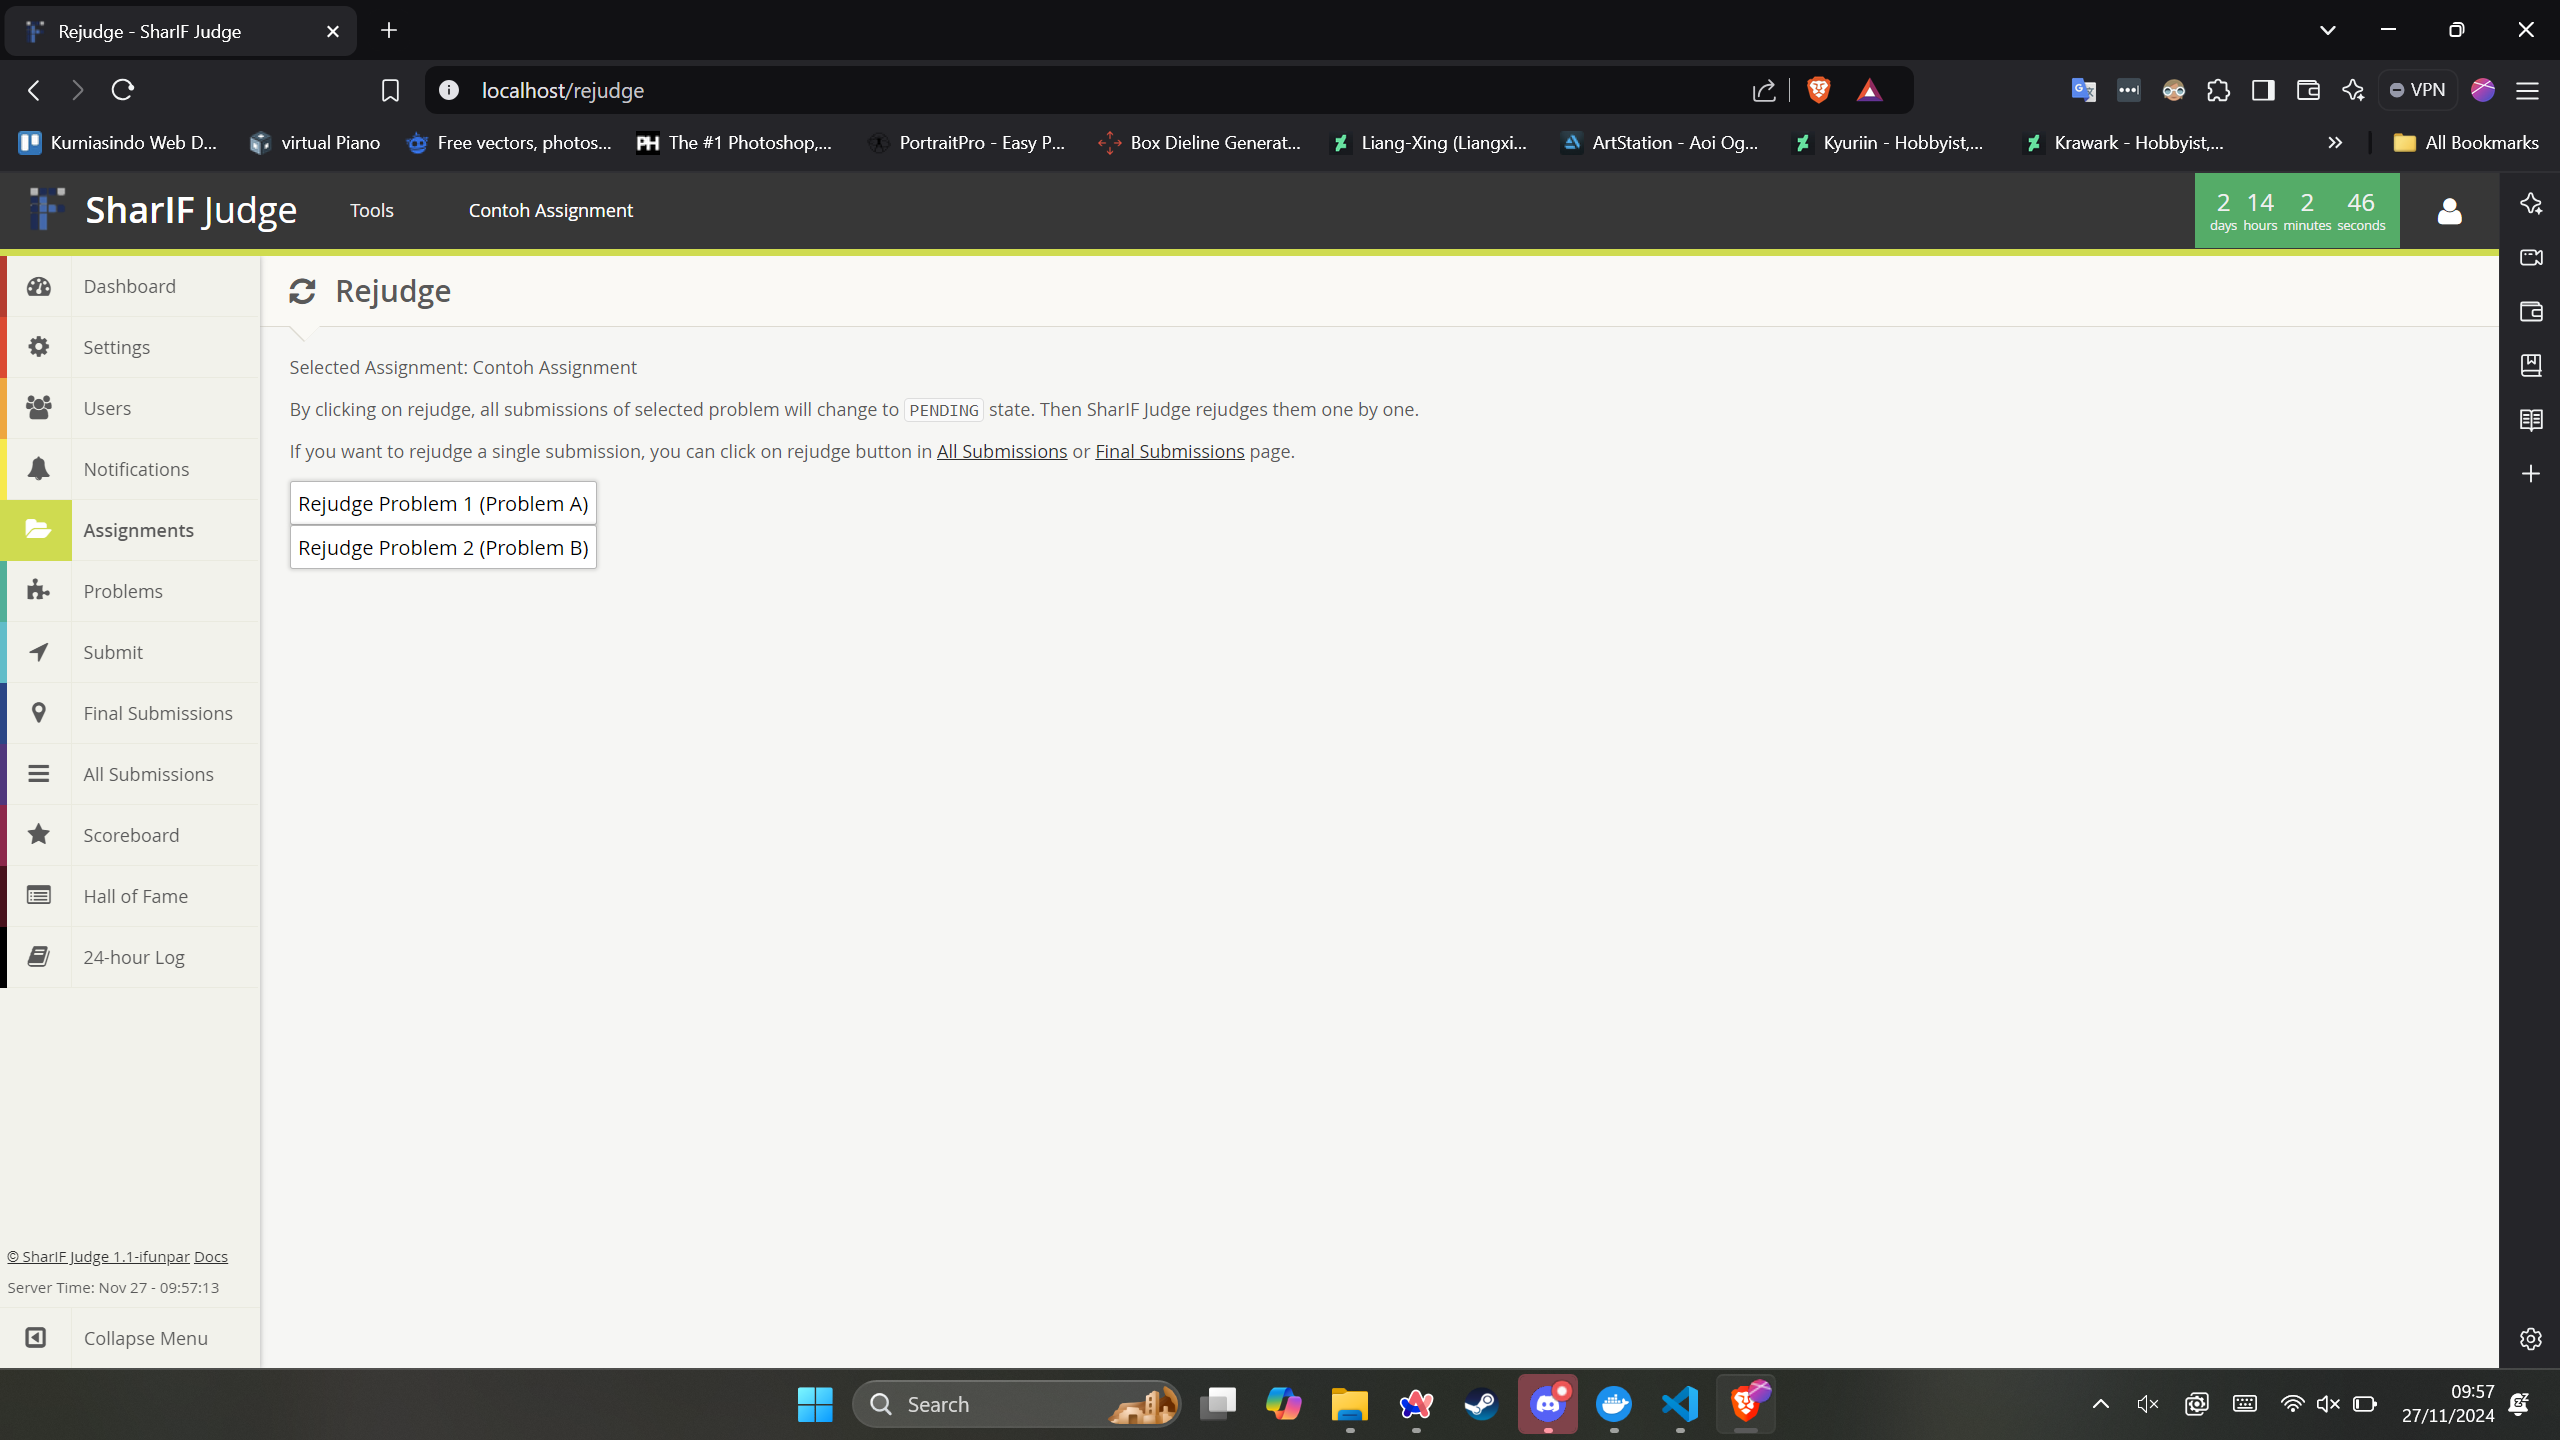
\includegraphics[width=0.8\textwidth]{views/rejudge.png}
					                        \caption{Halaman Rejudge}
					                        \label{fig:3:1:1:rejudge}
				                        \end{figure}

			                  \end{itemize}

			            \item \verb|Scoreboard.php| \\
			                  \textit{Controller} \verb|Queueprocess.php| hanya memiliki satu fungsi yaitu \verb|index()| yang akan menampilkan \textit{view} \verb|scoreboard.twig| dengan data dari \verb|Scoreboard_model|. Gambar \ref{fig:3:1:1:scoreboard} menunjukkan hasil halaman Scoreboard.

			                  \begin{figure}[H]
				                  \centering
				                  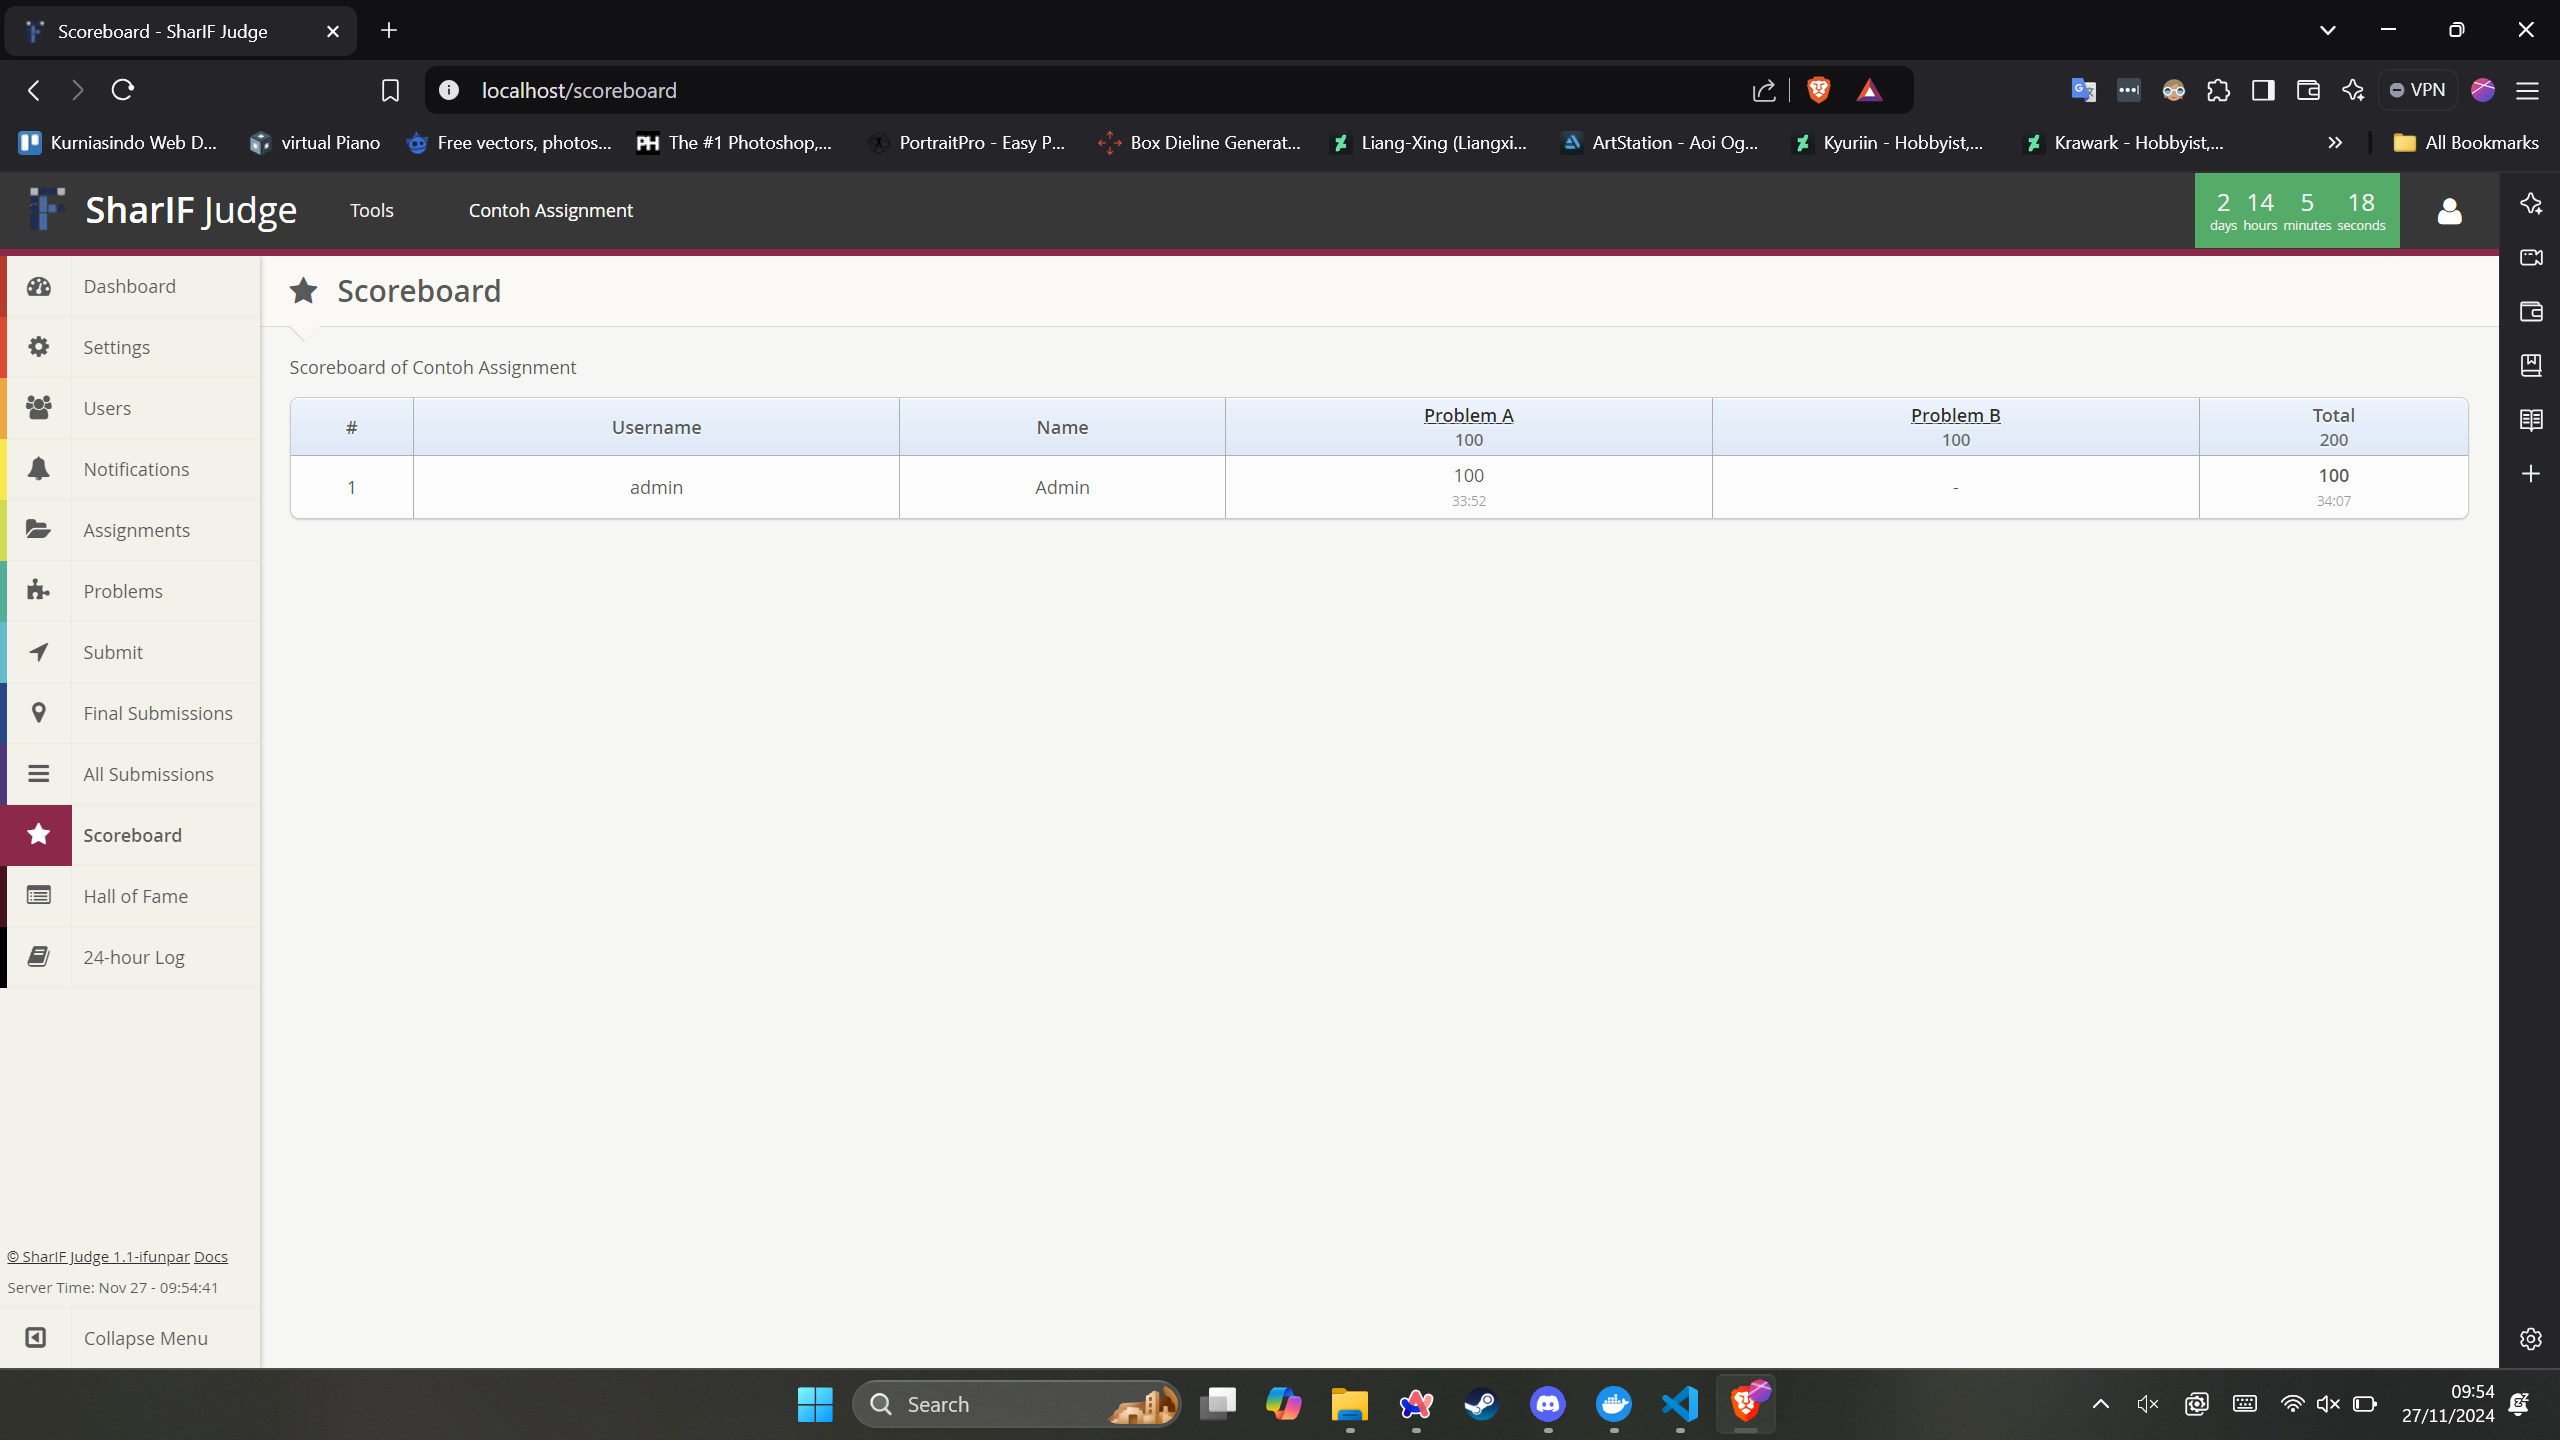
\includegraphics[width=0.8\textwidth]{views/scoreboard.png}
				                  \caption{Halaman Scoreboard}
				                  \label{fig:3:1:1:scoreboard}
			                  \end{figure}

			            \item \verb|Server_time.php| \\
			                  \textit{Controller} \verb|Queueprocess.php| hanya memiliki satu fungsi yaitu \verb|index()| yang akan mencetak waktu pada \textit{server}, waktu akan digunakan untuk sinkronisasi waktu.

			            \item \verb|Settings.php| \\
			                  Berikut fungsi dengan penjelasannya pada \textit{controller} \verb|Settings.php|:

			                  \begin{itemize}
				                  \item \verb|update()| \\
				                        Memperbaharui \textit{settings} dari masukkan pengguna.
				                  \item \verb|index()| \\
				                        Mendapatkan data dari \verb|Settings_model| dan menampilkan \textit{view} \verb|settings.twig|. Jika terdapat \textit{error setting} pada sistem, akan ditampilkan juga pada \textit{view} tersebut. Gambar \ref{fig:3:1:1:settings} menunjukkan hasil halaman Users.

				                        \begin{figure}[H]
					                        \centering
					                        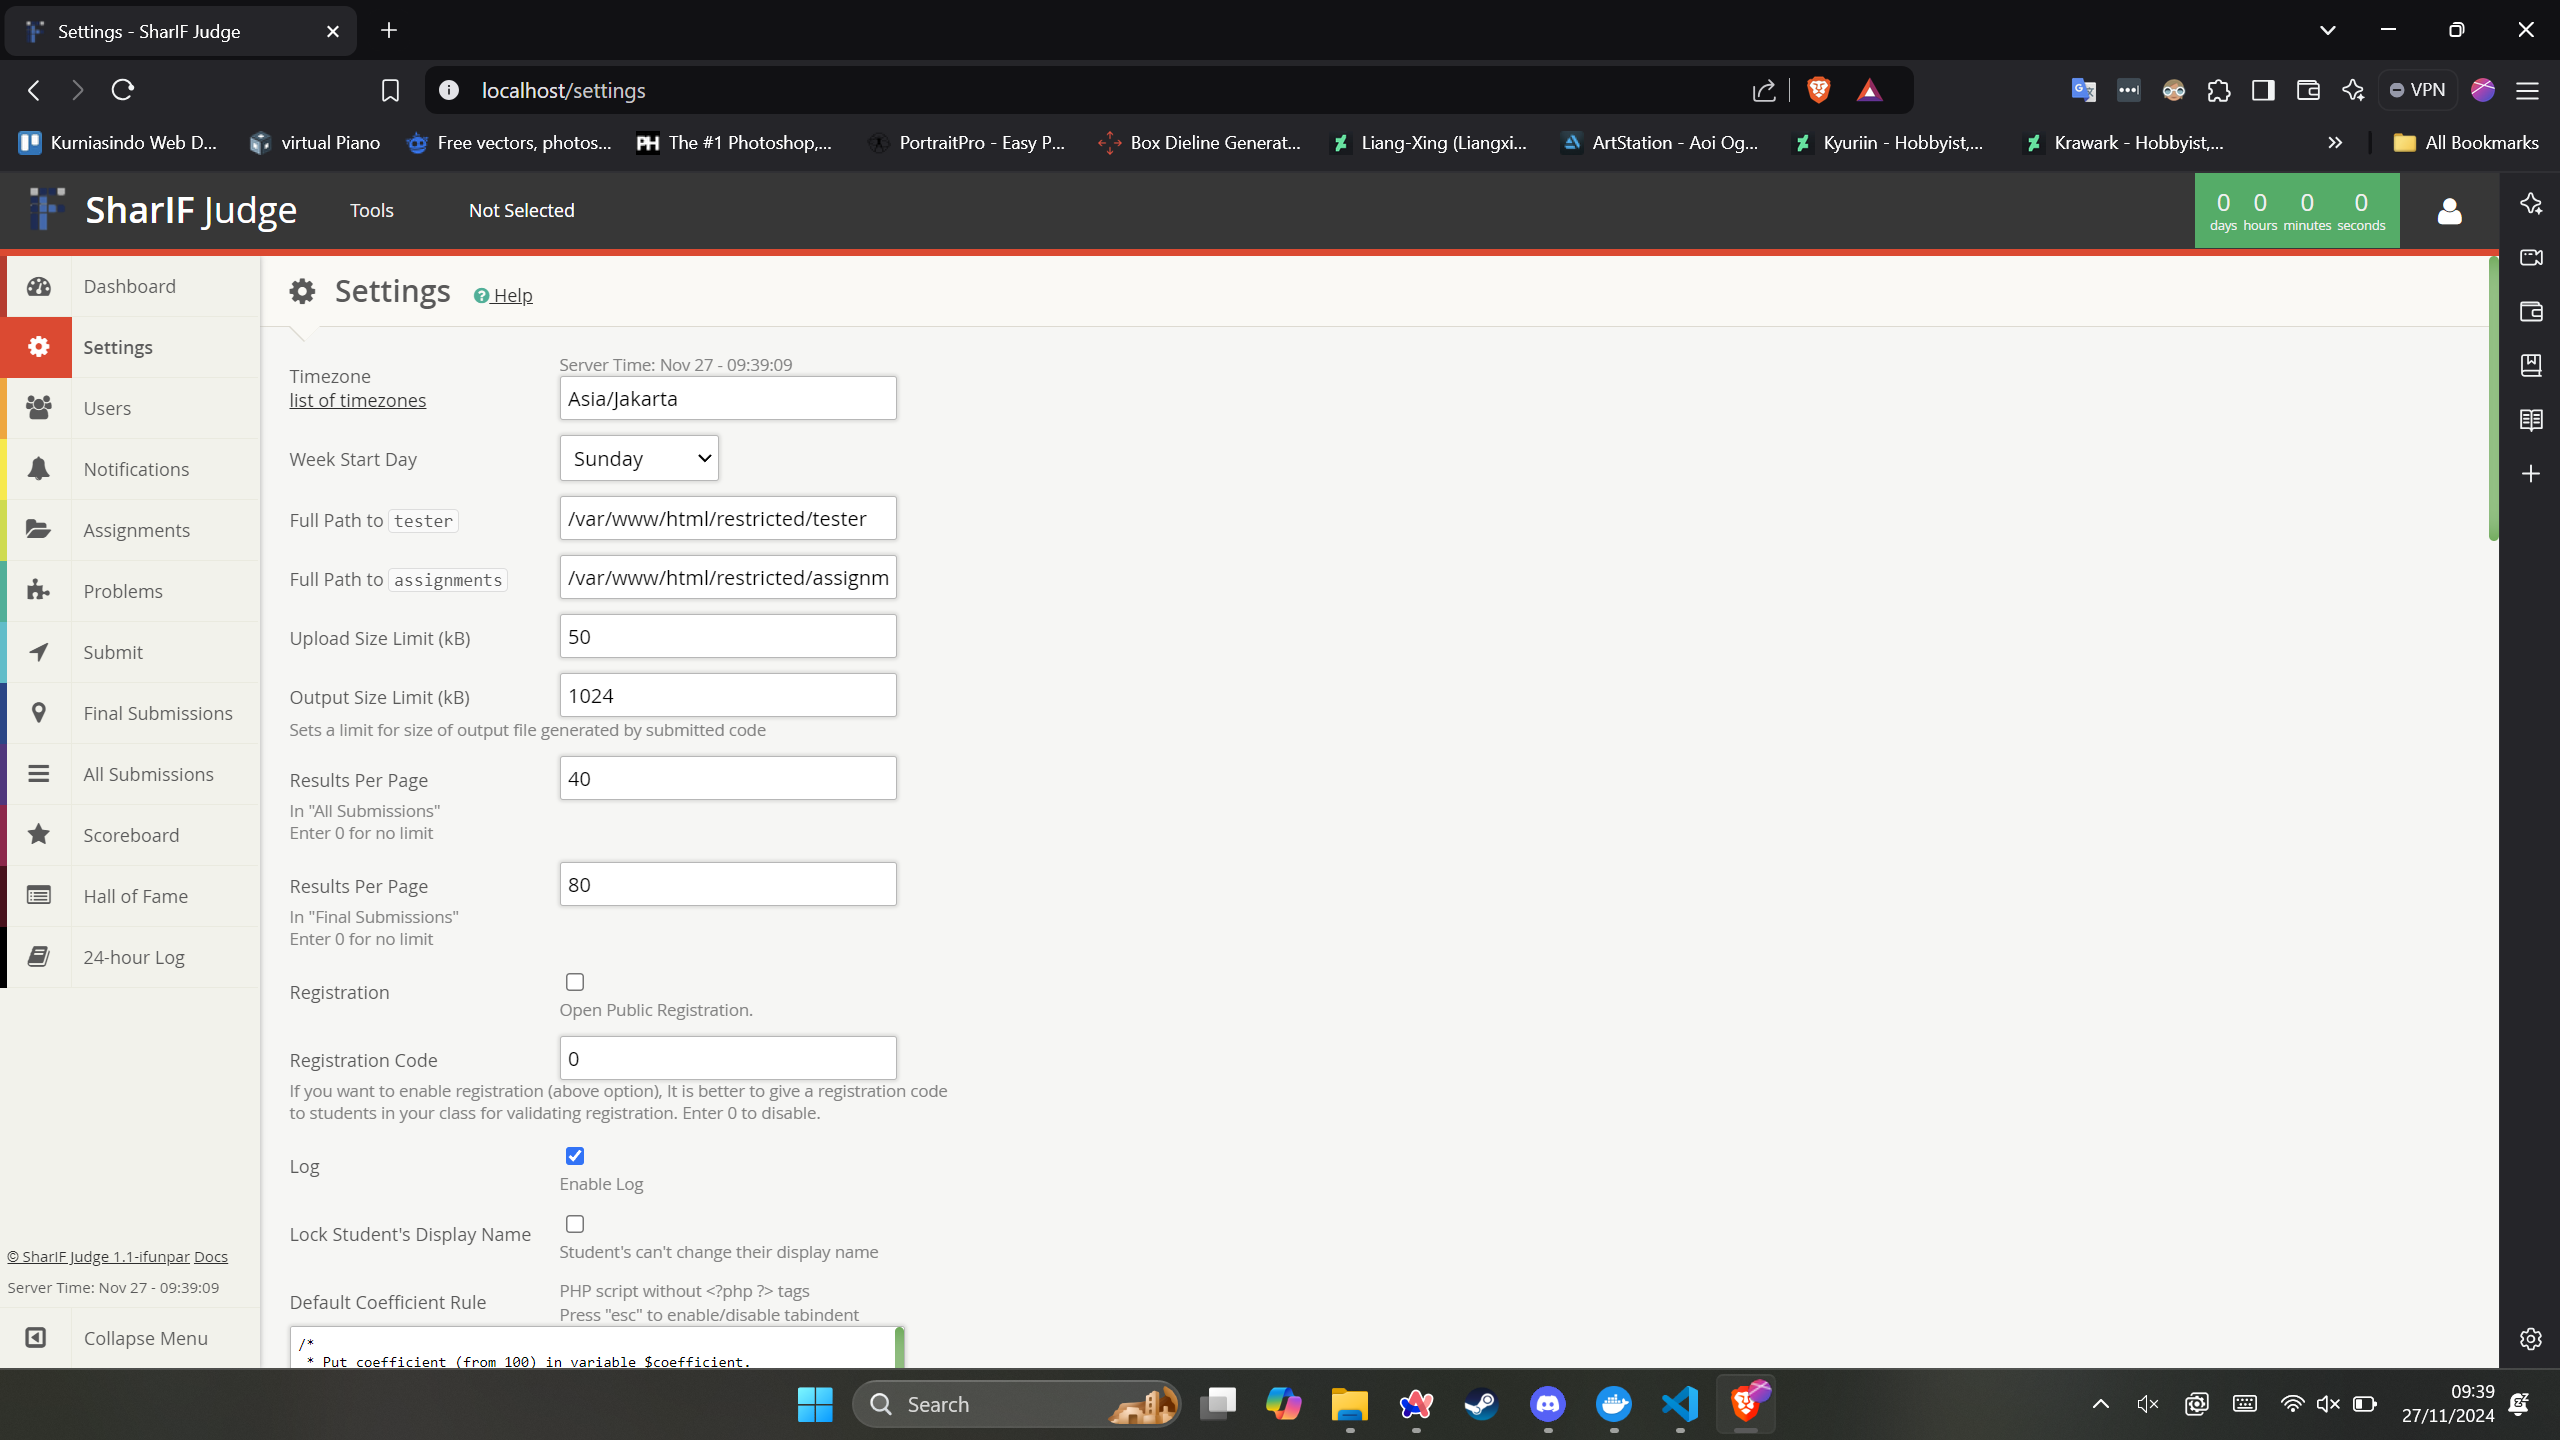
\includegraphics[width=0.8\textwidth]{views/settings.png}
					                        \caption{Halaman Settings}
					                        \label{fig:3:1:1:settings}
				                        \end{figure}

			                  \end{itemize}

			            \item \verb|Submissions.php| \\
			                  Berikut fungsi dengan penjelasannya pada \textit{controller} \verb|Submissions.php|:

			                  \begin{itemize}
				                  \item \verb|the_final()| \\
				                        Mendapatkan data dari \verb|Submit_model| untuk mendapatkan \textit{final submission} dan menampilkan halaman \verb|submission.twig| berisi \textit{final submission}. Gambar \ref{fig:3:1:1:final} menunjukkan halaman Final Submissions .
				                        \begin{figure}[H]
					                        \centering
					                        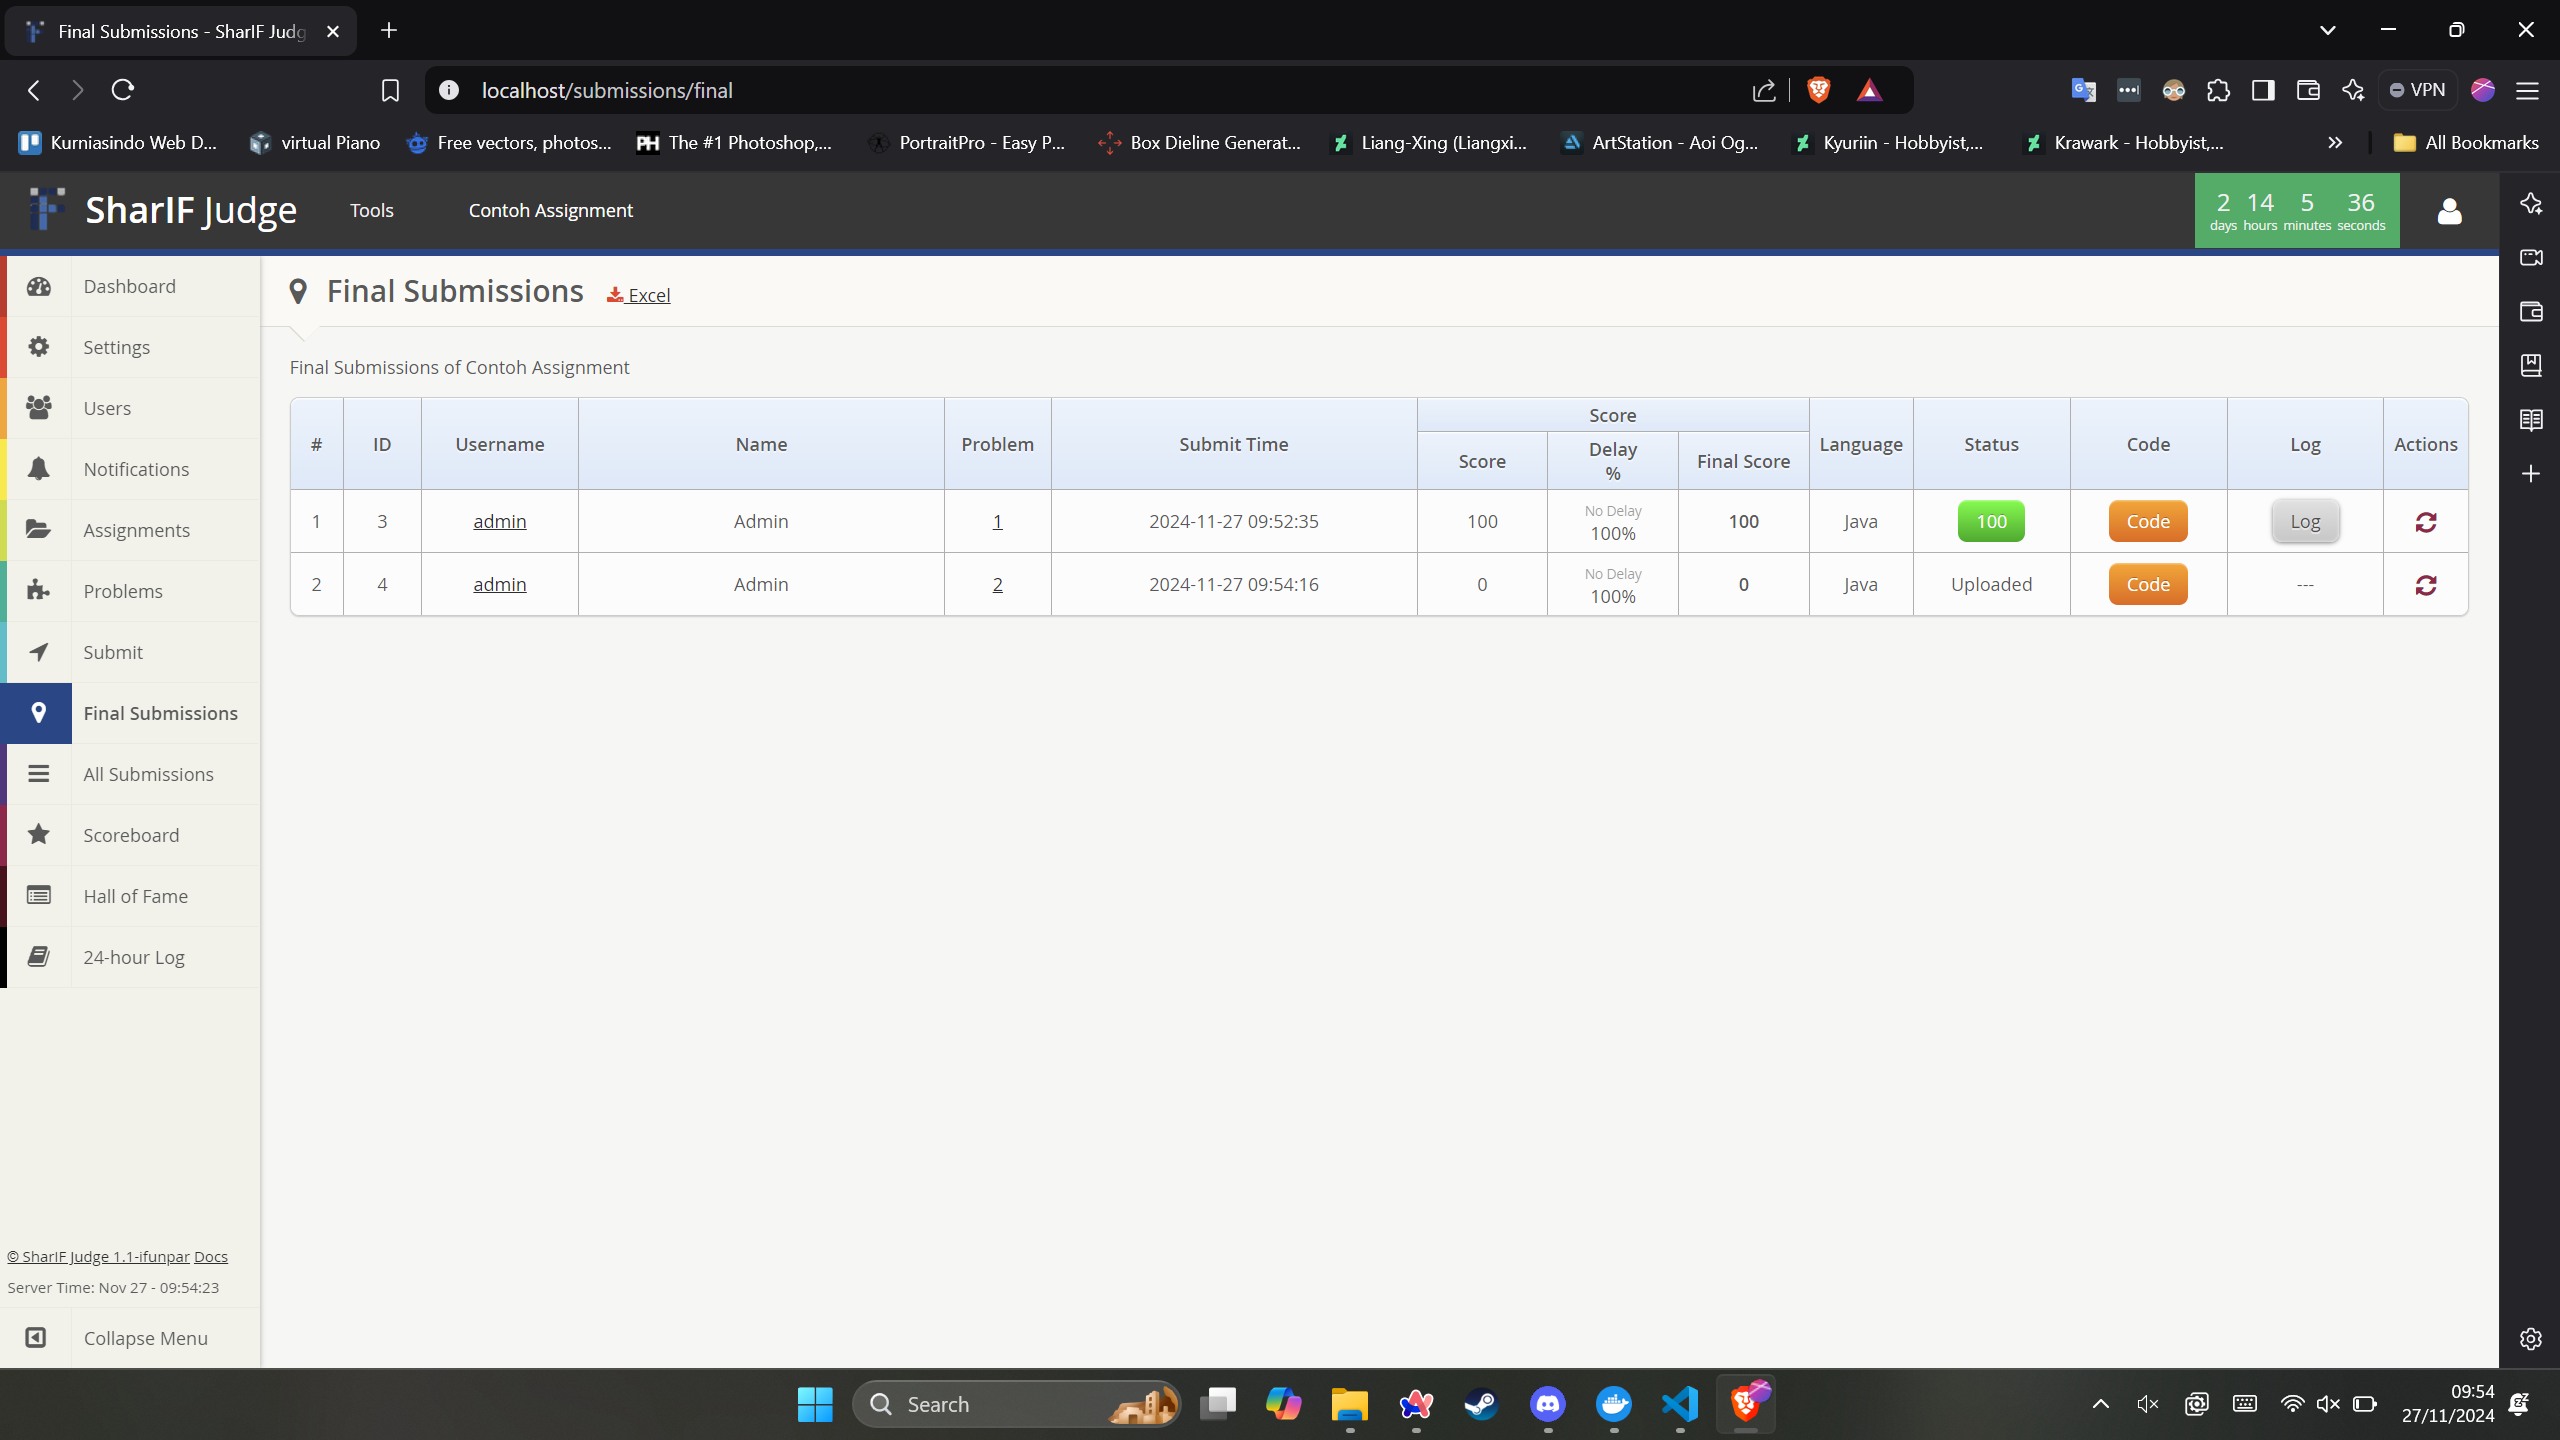
\includegraphics[width=0.8\textwidth]{views/final_submissions.png}
					                        \caption{Halaman Final Submissions}
					                        \label{fig:3:1:1:final}
				                        \end{figure}
				                  \item \verb|_download_excel($view)| \\
				                        Menggunakan \textit{library} PHPExcel untuk membuat sebuah \textit{file excel} dari \textit{submissions} yang akan diunduh pengguna.
				                  \item \verb|final_excel()| \\
				                        Menggunakan fungsi \verb|_download_excel| untuk mendownload \textit{final submission}.
				                  \item \verb|all_excel()| \\
				                        Menggunakan fungsi \verb|_download_excel| untuk mendownload seluruh \textit{submission}.
				                  \item \verb|select()| \\
				                        Menggunakan \textit{ajax request} untuk memilih \textit{submission} yang akan dikumpulkan atau menjadi \textit{final}.
				                  \item \verb|_check_type($type)| \\
				                        Melakukan validasi tipe \textit{submission} yang dikumpulkan.
				                  \item \verb|view_code()| \\
				                        Digunakan untuk melihat kode, melihat hasil kode, atau melihat \textit{log} sebuah \textit{submission}.
				                  \item \verb|download_file()| \\
				                        Mengunduh \textit{file} kode sebuah \textit{submission}.

				                  \item \verb|all()| \\
				                        Mendapatkan data dari \verb|Submit_model| untuk mendapatkan seluruh \textit{submission} dan menampilkan halaman \verb|submission.twig| berisi semua \textit{submission}. Gambar \ref{fig:3:1:1:all} menunjukkan halaman All Submissions .

				                        \begin{figure}[H]
					                        \centering
					                        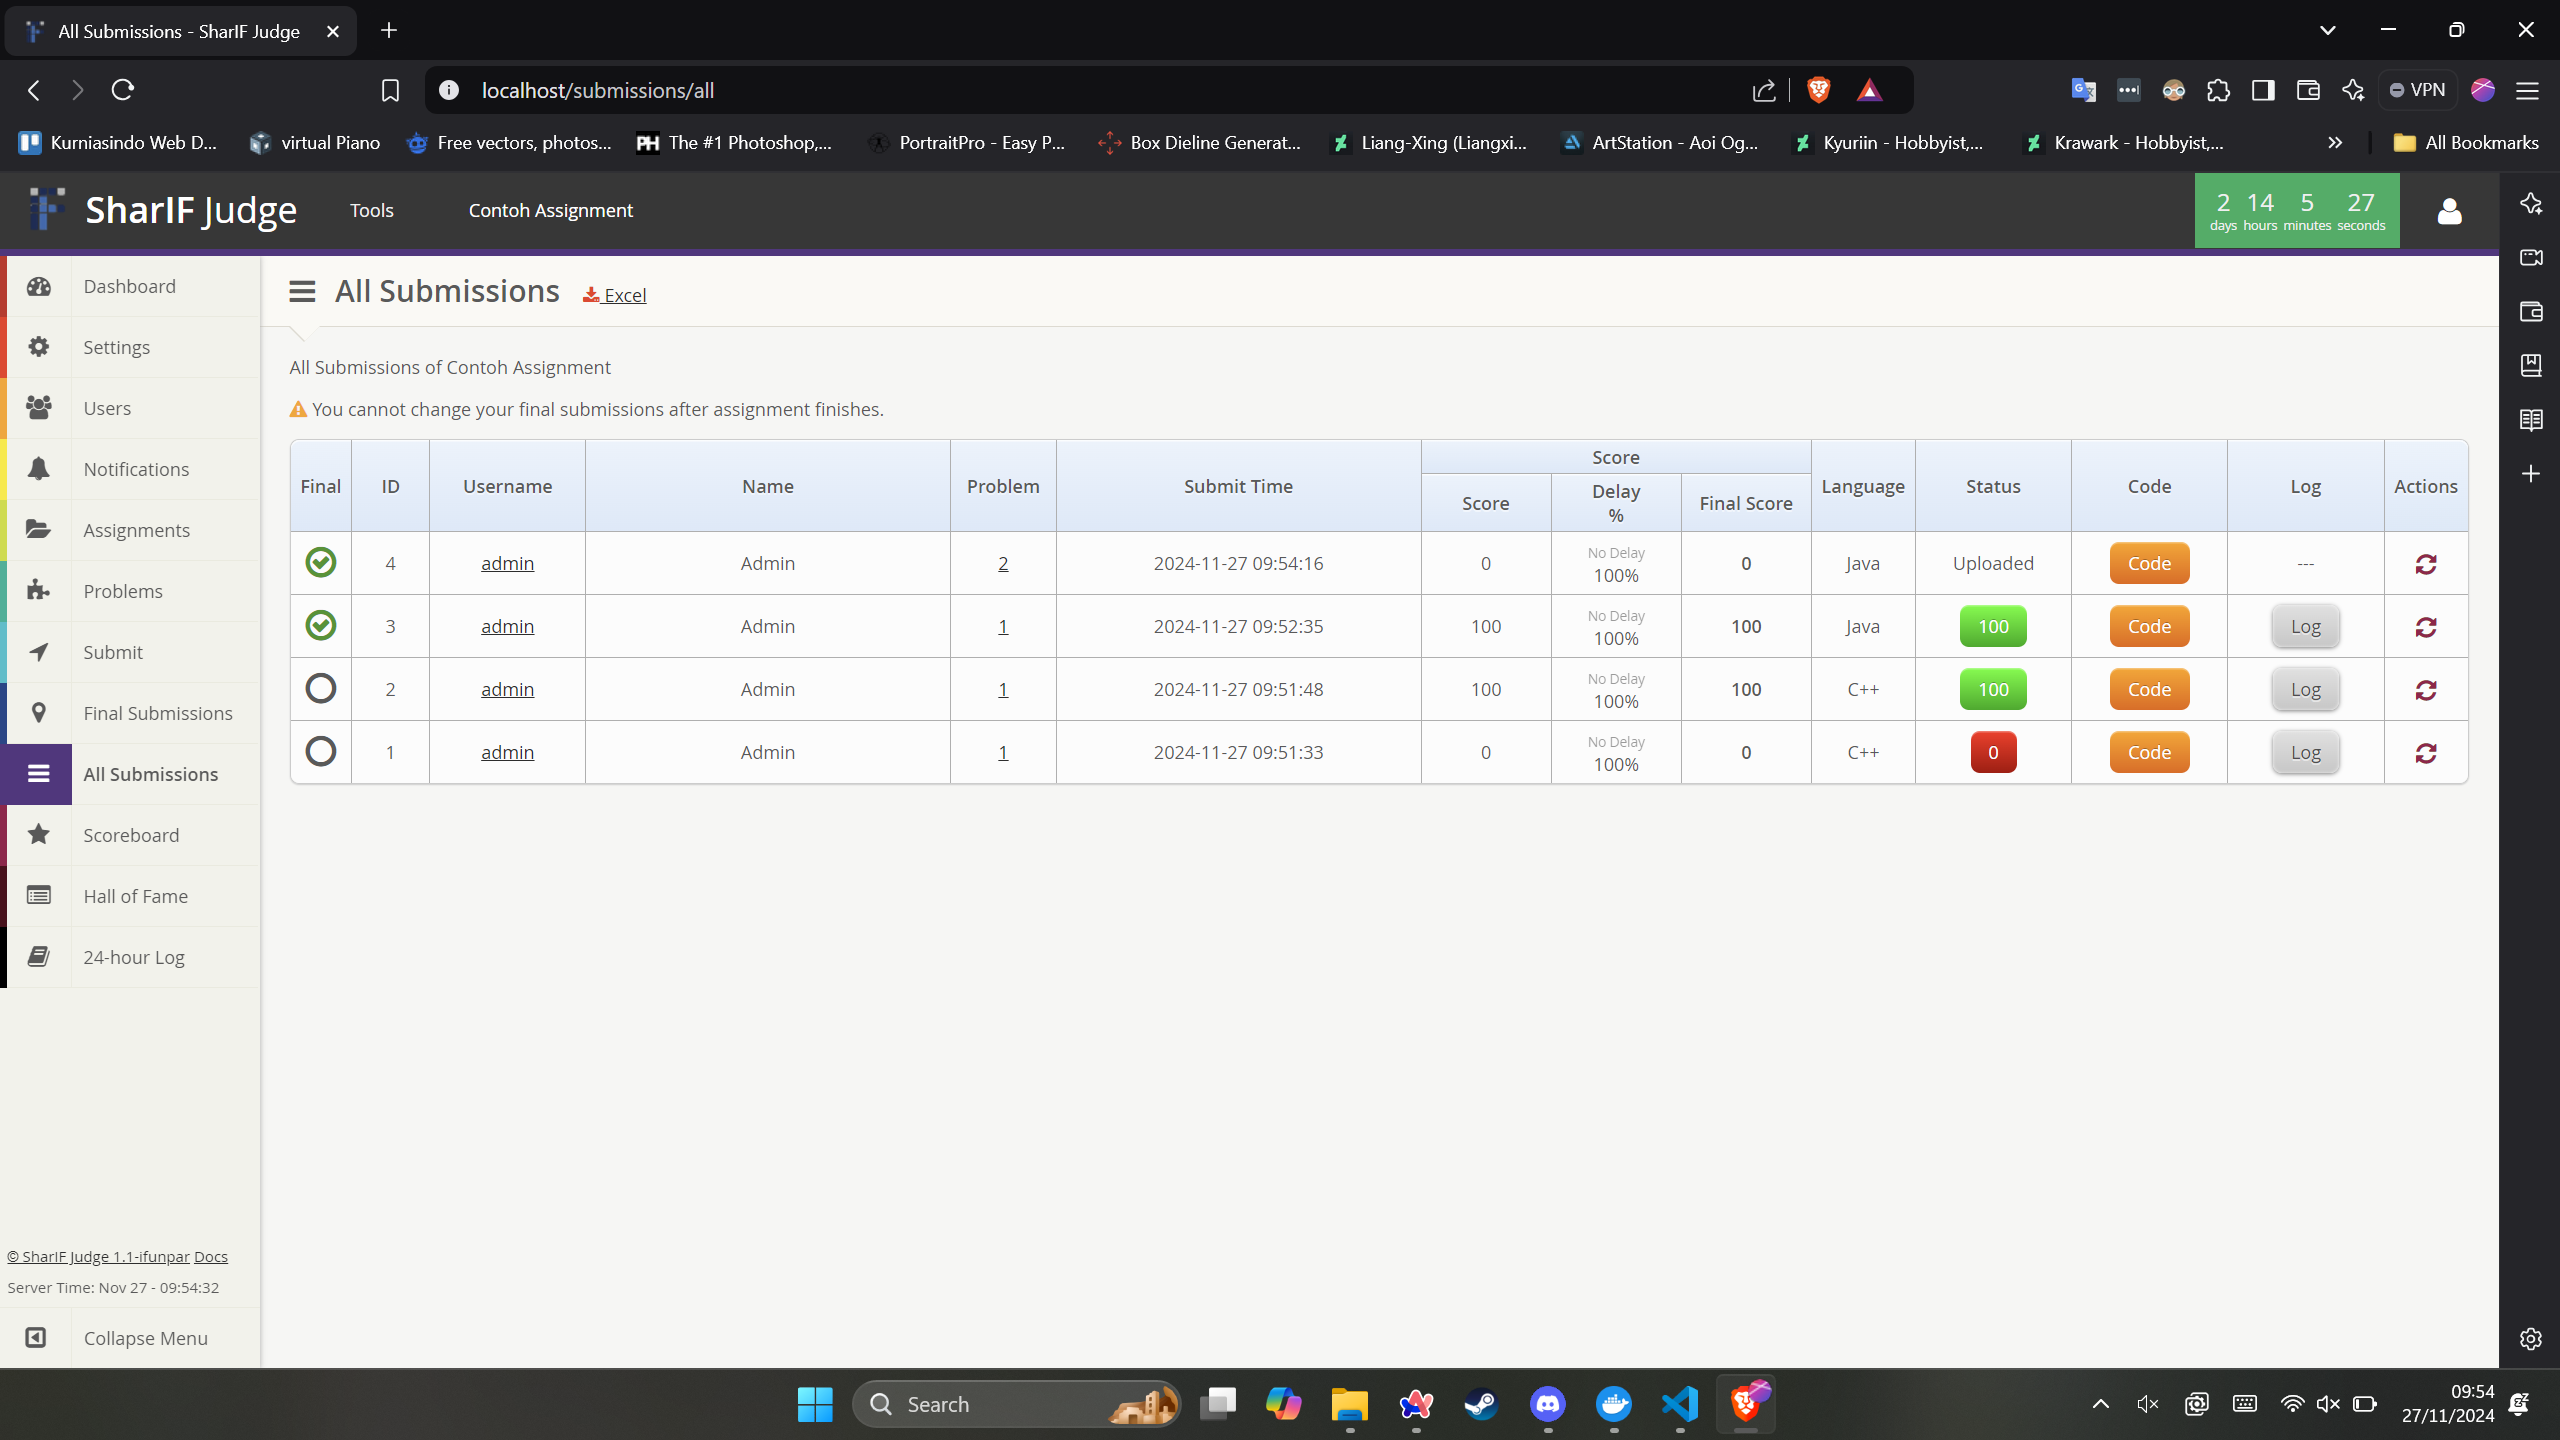
\includegraphics[width=0.8\textwidth]{views/all_submissions.png}
					                        \caption{Halaman All Submissions}
					                        \label{fig:3:1:1:all}
				                        \end{figure}
			                  \end{itemize}

			            \item \verb|Submit.php| \\
			                  Berikut fungsi dengan penjelasannya pada \textit{controller} \verb|Submit.php|:

			                  \begin{itemize}
				                  \item \verb|_language_to_type($language)| \\
				                        Mengembalikan kode singkat dari \verb|$language| dipilih.
				                  \item \verb|_language_to_ext($language)| \\
				                        Mengembalikan extensi file dari \verb|$language| yang dipilih.
				                  \item \verb|_match($type, $extension)| \\
				                        Melakukan validasi untuk \verb|$type| dan \verb|$extension| agar sesuai.
				                  \item \verb|_check_language($str)| \\
				                        Melakukan validasi sudah dipilihannya bahasa.
				                  \item \verb|_upload()| \\
				                        Menyimpan jawaban pengguna yang dikirim dan menambahkannya ke dalam \textit{queue} untuk dinilai jika bukan \textit{upload only problem}.
				                  \item \verb|load($problem_id)| \\
				                        Mendapatkan isi file dan menaruh isi file ke editor kode.
				                  \item \verb|save($type)| \\
				                        Menyimpan isi editor kode ke dalam \textit{server} dan menjalankan atau mengumpulkan jika diinginkan.
				                  \item \verb|_submit($data, $problem_id, $language, $user_dir)| \\
				                        Menambahkan kode ke dalam \textit{submission} untuk dinilai.
				                  \item \verb|_execute($data, $problem_id, $language, $user_dir)| \\
				                        Menambahkan kode ke dalam \textit{queue} untuk di jalankan saja.
				                  \item \verb|get_output($problem_id)| \\
				                        Mendapatkan keluaran dari kode yang telah dijalankan sebagai hasil eksekusi.
				                  \item \verb|index()| \\
				                        Mendapatkan data dari \textit{model} \verb|Assignments_model| untuk mendapatkan \textit{problem} dan data lainnya. Semua data akan dimasukkan dalam \textit{view} \verb|submit.twig|. Gambar \ref{fig:3:1:1:submit} menunjukkan hasil halaman Submit. Halaman ini terdapat editor kode yang sudah di implementasikan oleh Nicholas Aditya Halim\footnote{Halim, N.~A. (2021) {Implementasi Editor Kode pada SharIF Judge}. Skripsi. Universitas Katolik Parahyangan,  Indonesia.}.

				                        \begin{figure}[H]
					                        \centering
					                        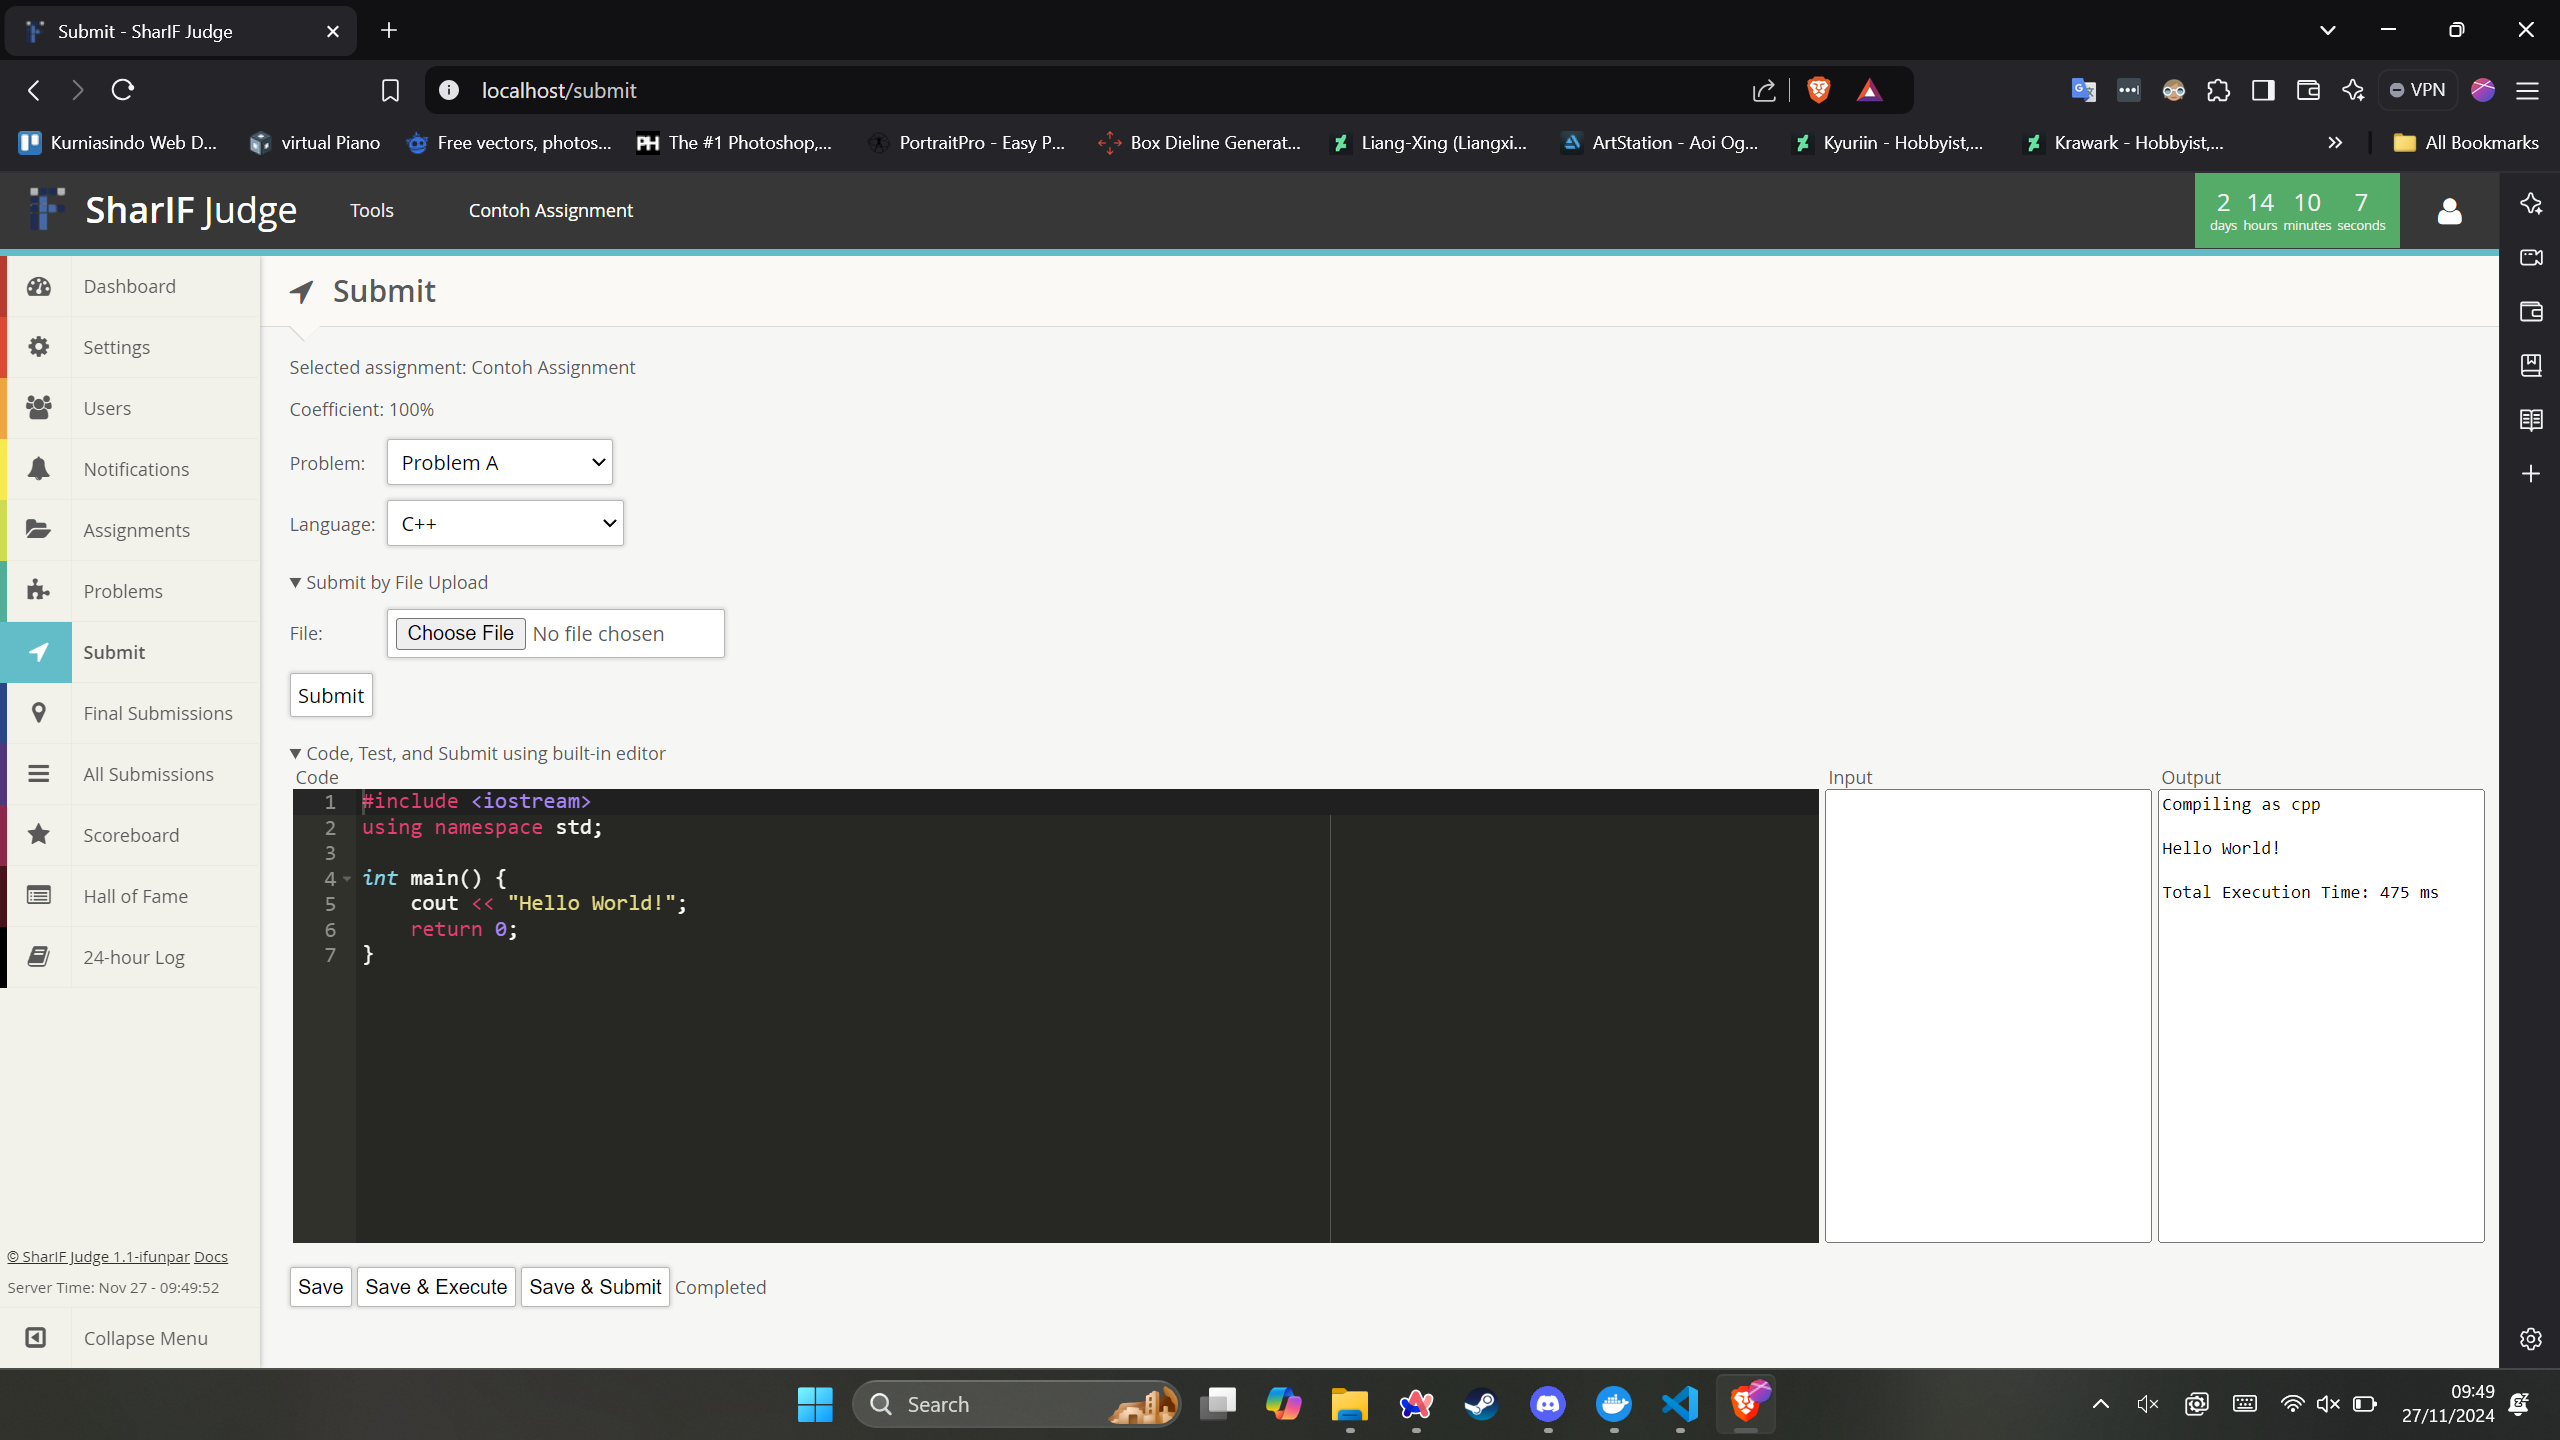
\includegraphics[width=0.75\textwidth]{views/submit.png}
					                        \caption{Halaman Submit}
					                        \label{fig:3:1:1:submit}
				                        \end{figure}

			                  \end{itemize}

			            \item \verb|User.php| \\
			                  Berikut fungsi dengan penjelasannya pada \textit{controller} \verb|User.php|:

			                  \begin{itemize}
				                  \item \verb|add()| \\
				                        Menambahkan \textit{user} baru ke dalam \textit{sistem}.
				                  \item \verb|delete()| \\
				                        Menghapus sebuah \textit{user}.
				                  \item \verb|delete_submissions()| \\
				                        Menghapus seluruh \textit{submissions} dari sebuah \textit{user}.
				                  \item \verb|list_excel()| \\
				                        Menggunakan \textit{library} PHPExcel untuk membuat sebuah file excel dari seluruh daftar \textit{user} yang akan diunduh pengguna.
				                  \item \verb|index()| \\
				                        Fungsi ini digunakan akan mendapatkan data dari \verb|User_model| dan menunjukkan \textit{view} \verb|users.twig| dengan data tersebut. Gambar \ref{fig:3:1:1:users} menunjukkan hasil halaman Users. Pada halaman ini terdapat daftar seluruh \textit{user} yang terdaftar pada SharIF Judge. Pengguna dapat membuat, memperbaharui, dan menghapus \textit{user}.

				                        \begin{figure}[H]
					                        \centering
					                        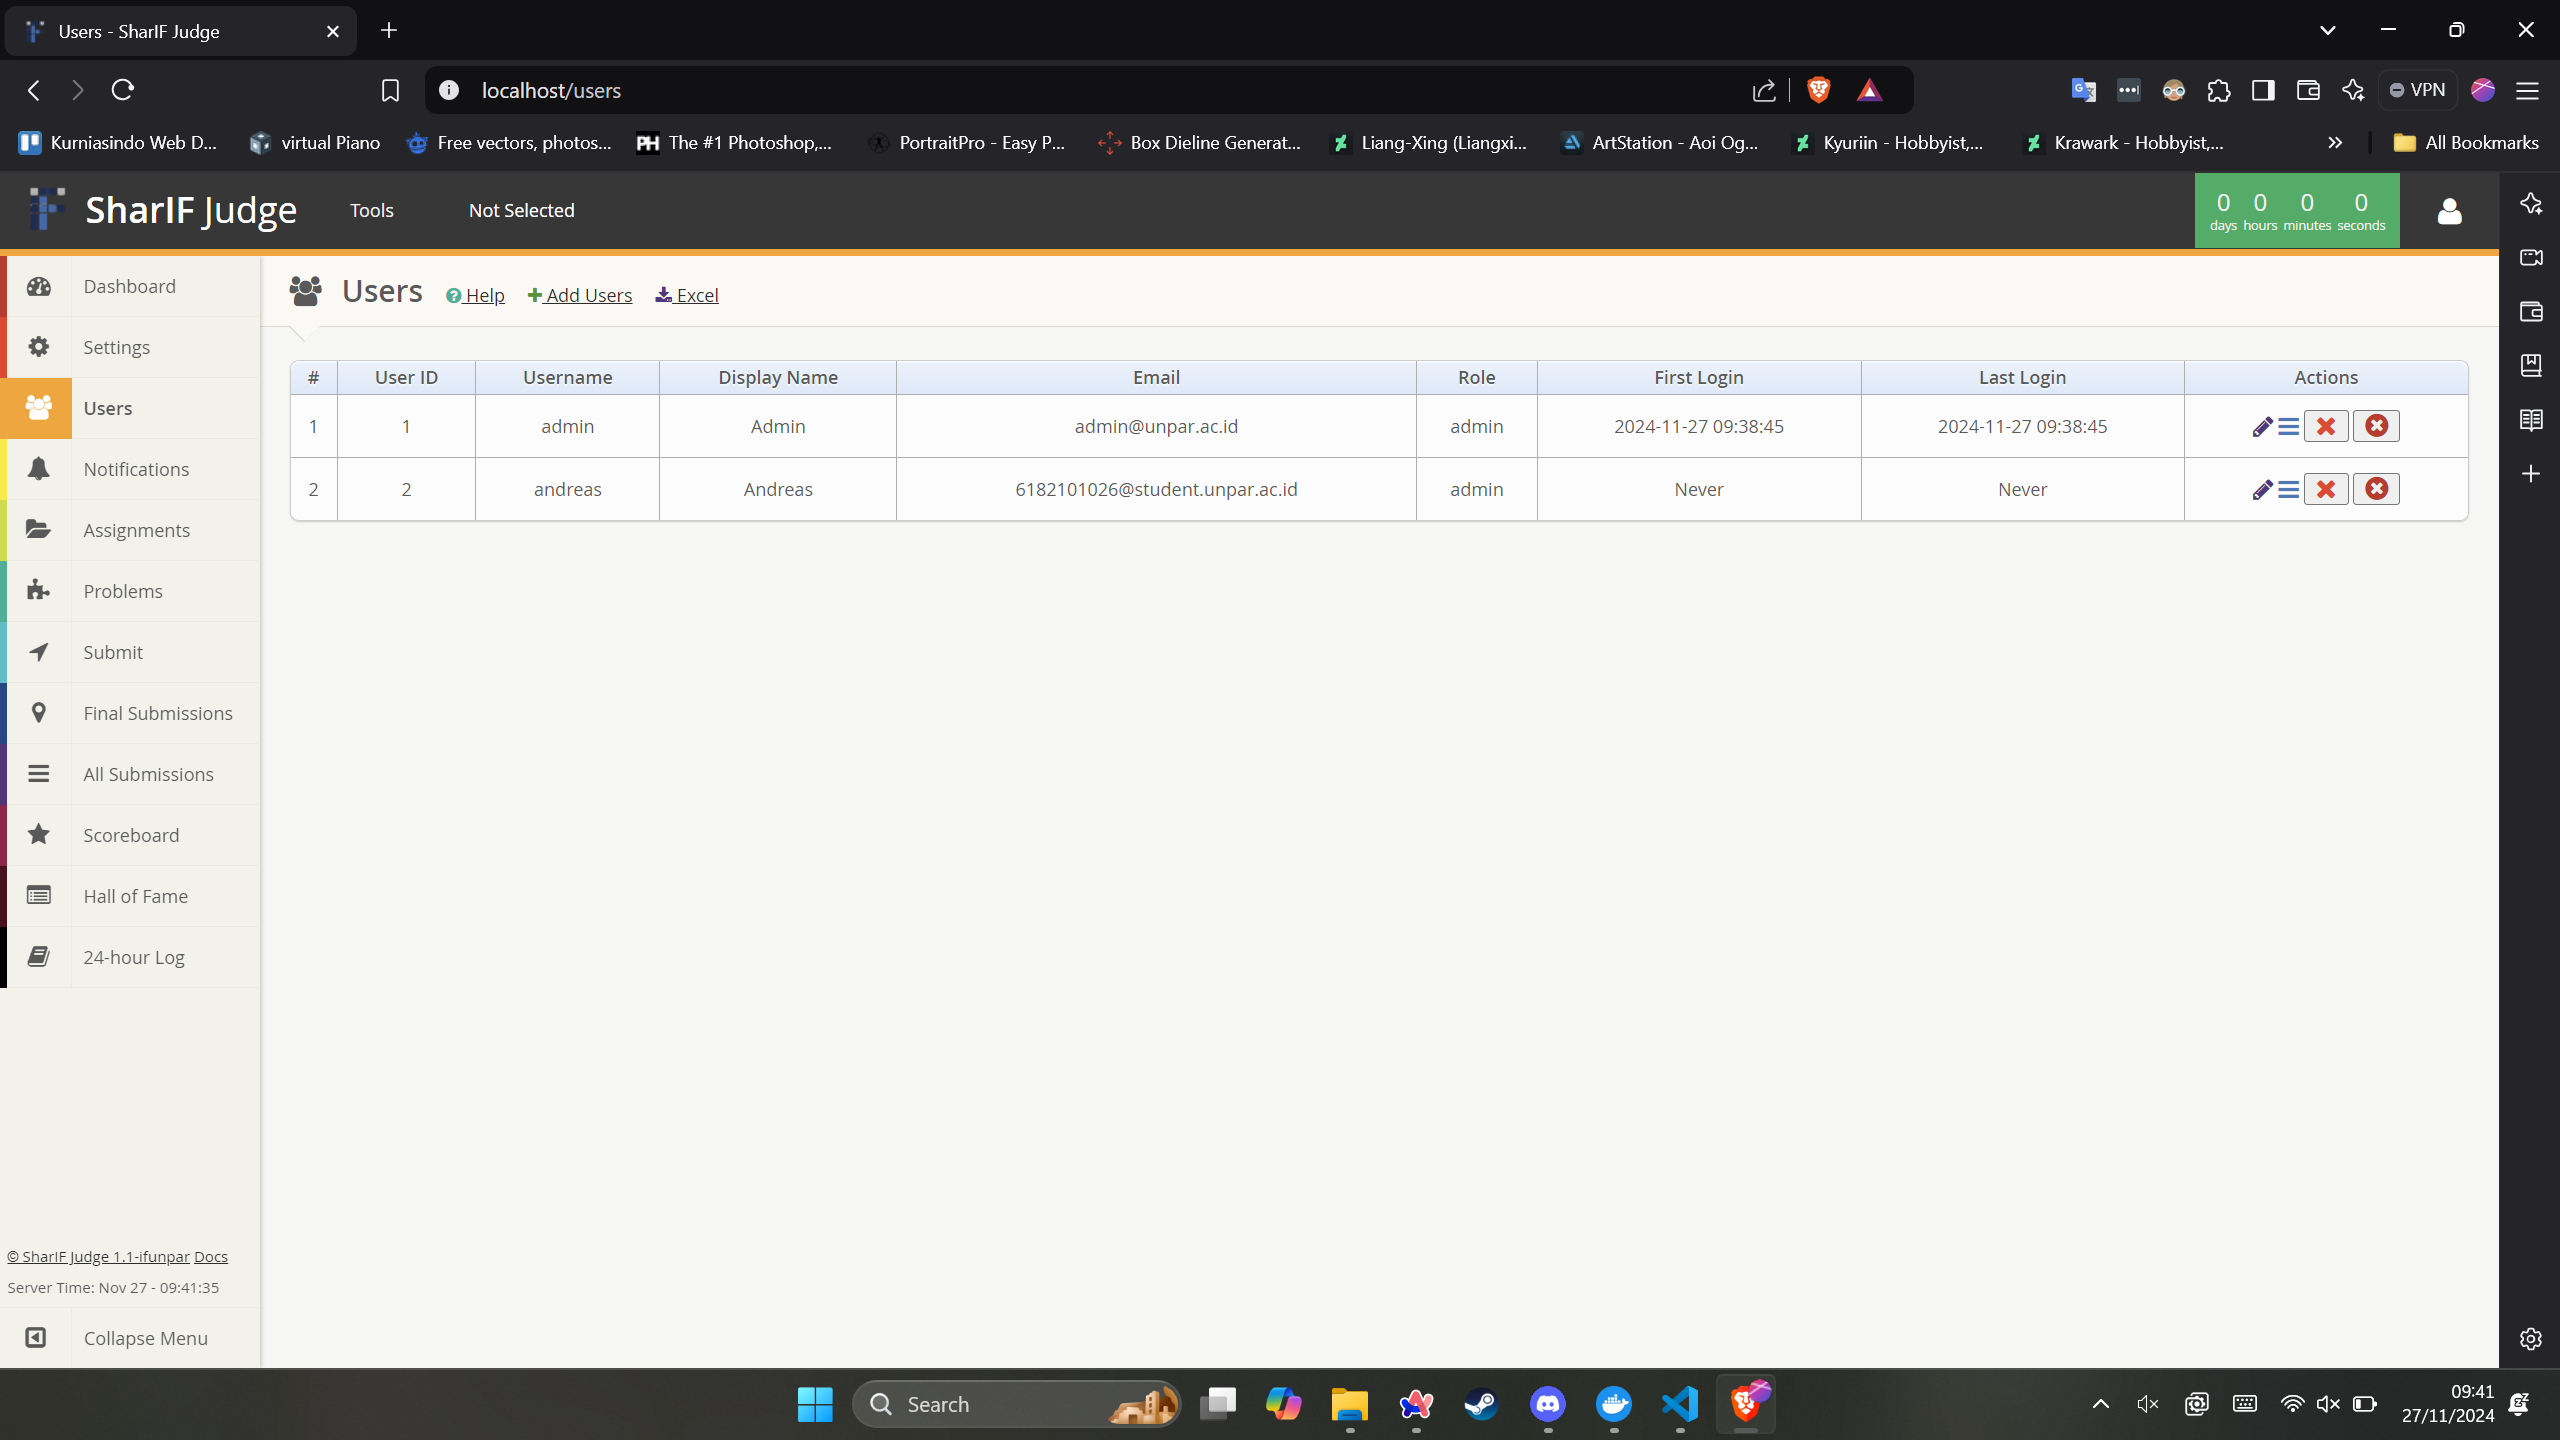
\includegraphics[width=0.8\textwidth]{views/users.png}
					                        \caption{Halaman Users}
					                        \label{fig:3:1:1:users}
				                        \end{figure}


			                  \end{itemize}

		            \end{itemize}
	      \end{itemize}

	\item \textbf{Melakukan studi literatur mengenai Twig\footnote{Dokumentasi twig. https://twig.symfony.com/doc/3.x/(10 Desember 2024)}.}\\
	      {\bf Status :} baru ditambahkan pada semester ini\\
	      {\bf Hasil :} Sudah melakukan studi mengenai menggunakan Twig.

	      Berikut merupakan hasil studi penggunaan Twig:

	      Twig merupakan sebuah \textit{template engine} untuk PHP. Ada beberapa \textit{expression}, \textit{expression}, atau \textit{statement} yang ditemupakan pada template Twig adalah sebagai berikut:
	      \begin{itemize}
		      \item Pewarisan \textit{Template}
		      \item Struktur Kontrol (mengunaan kondisional, \textit{looping})
		      \item Filter
		      \item Variable pada PHP
	      \end{itemize}

	      Pada saat template dievaluasi, semua \textit{variable} atau \textit{expression} akan dibuah menjadi value dan \textit{tag} yang mengontrol logika template. Berikut contoh kode menggunakan \textit{twig}.

	      \begin{lstlisting}[language={php}, caption={Contoh template Twig}, label={kode:2:twig}]


	<ul id="navigation">
	
		<li>
			<a href="{{item.href}}">
				&nbsp;&nbsp;
				{{ item.caption|upper }}
			</a>
		</li>
	
	</ul>

			\end{lstlisting}

	      Kode \ref{kode:2:twig} merupakan contoh sebuah template Twig. Terdapat dua jenis \textit{delimiter}, yaitu \verb|| dan \verb|{{ ... }}|. \textit{Delimiter} \verb|| digunakan untuk Menjalankan sebuah \textit{statement} seperti \textit{for-loops}, sedangkan \textit{delimiter} \verb|{{ ... }}| digunakan untuk mengubah sebuah \textit{variable} atau \textit{expression} menjadi sebuah html biasa dengan nilai \textit{variable} atau \textit{expression} tersebut.


	\item \textbf{Melakukan studi mengenai cara penyimpanan rekaman ketikan.} \\
	      {\bf Status :} Ada sejak rencana kerja skripsi.\\
	      {\bf Hasil :} Sudah melakukan sebagian studi mengenai penyimpanan rekaman ketikan.

	      Berikut merupakan kesimpulan yang didapat dalam penyimpanan rekaman ketikan.

	      Sebelum ketikan dapat di putar kembali, dibutuhkannya fitur untuk merekam segala \textit{event} yang terjadi pada masukkan tersebut. \textit{Event} yang sudah direkam akan disimpan bersama dengan waktu saat di terjadinya \textit{event} tersebut. Penyimpanan rekaman juga akan disimpan pada folder yang sama dengan penyimpanan kode submission seperti yang dijelaskan pada bagian \ref{sub:3:1:penyimpanankode} dengan nama file \verb|recording|. Pemimpanan perekaman akan memiliki format sebagai berikut:

	      \begin{center}
		      \verb|<timeline>: {event: <event>, data: <payload>}|
	      \end{center}

	      \verb|<timeline>| akan menunjukkan pada milidetik berapa \textit{event} terjadi dengan menggunakan fungsi \verb|Date.| \\ \verb|now()| pada \textit{Javascript}. sedangkan \verb|<event>| dan \verb|<payload>| merupakan data \textit{event} yang terjadi. \verb|<pay| \\ \verb|load>| akan disesuaikan dengan \textit{event} yang terjadi. Sebagai contoh untuk \textit{event insert} huruf `a' akan di tuliskan menjadi sebagai berikut:

	      \begin{center}
		      \verb|1733335637486: {event: "insert", data: "a"}|
	      \end{center}

	      Penyimpanan \textit{event} akan di lakukan oleh \textit{Controller} \verb|Submit| yang akan menyimpan \textit{file} pada saat kode disimpan. Maka fungsi yang akan dimodifikasi adalah fungsi \verb|save()|.

	      Untuk tugas akhir 2 akan melakukan studi mengenai tipe file yang akan digunakan seperti JSON, BSON, atau Protocol Buffer. Hal ini tidak dapat diselesaikan pada tugas akhir ini karena pada tugas akhir 1 memfokuskan analisis mengenai cara kerja berbagai \textit{framework} yang terdapat SharIF Judge dan juga mempelajari SharIF Judgenya juga.

	\item \textbf{Memodelkan dan merencanakan perubahan pada structur website dan database pada SharIF-Judge.} \\
	      {\bf Status :} Ada sejak rencana kerja skripsi.\\
	      {\bf Hasil :} Sudah melakukan perencanaan perubahan pada structur website dan database.

	      Berikut perencaan yang didapat:

	      Pada SharIF Judge akan ditambahkan dalam beberapa file yaitu file \verb|shj_submit.js| yang mengatasi bagian \textit{client side} untuk mengotomasikan rekaman \textit{event}. Selanjutnya akan ada perubahan yang dilakukan saat editor kode di save, maka file yang berubah adalah \verb|shj_submit.js|, \textit{Controller} \verb|Submit.php|, dan \textit{Model} \verb|Submit_model.php|.

	      Pada sistem perekaman ketikan dibutuhkan penyimpanan untuk list recording yang tersedia dalam sistem dengan menyimpan ke dalam database. Maka dibutuhkan tabel baru dengan nama \verb|recording| yang memiliki beberapa \textit{fields} yaitu:

	      \begin{enumerate}
		      \item \verb|id|
		      \item \verb|username|
		      \item \verb|assignment|
		      \item \verb|problem|
		      \item \verb|time|
		      \item \verb|file_name|
	      \end{enumerate}

	      Pada SharIF Judge dibutuhkannya juga beberapa hal baru yaitu \textit{Controller} \verb|Recording.php|, \textit{View} \verb|recording.twig|, \textit{Model} \verb|Recording_model.php|, dan \textit{Javascript} \verb|shj_recording.js|.

	      \vspace{0.15cm}
	      \textit{Controller} \verb|Recording.php| akan memiliki beberapa fungsi utama yaitu:
	      \begin{itemize}
		      \item \verb|index()| \\
		            Fungsi \verb|index()| akan mengambil list recording sesuai dengan \textit{assignment} \textit{problem} yang dipilih dan mengembalikan \textit{view} \verb|recording.twig|
		      \item \verb|load_recording()| \\
		            Fungsi \verb|load_recording()| akan digunakan untuk mengambil file yang sudah di simpan pada server dan mengembalikannya.
	      \end{itemize}

	      \vspace{0.15cm}
	      Untuk \textit{model} \verb|Recording_model.php| akan memiliki beberapa fungsi utama yaitu:
	      \begin{itemize}
		      \item \verb|save_recording()| \\
		            Fungsi ini akan digunakan untuk menyimpan file recoding pada \textit{database} \verb|recoding|.
		      \item \verb|delete_recording()| \\
		            Fungsi ini akan digunakan untuk menghapus file recoding pada \textit{database} \verb|recoding|.
		      \item \verb|get_list_recording()| \\
		            Fungsi ini akan digunakan untuk mengembalikan \textit{list recoding} pada \textit{database}.
	      \end{itemize}

	      \vspace{0.15cm}
	      \textit{Javascript} yang akan dibuat pada \verb|shj_recording.js| akan memiliki berbagai fungsi yaitu sebagai berikut:

	      \begin{itemize}
		      \item Fungsi untuk memilih \textit{user} dan \textit{problem} yang ditampilkan.
		      \item Fungsi ajax untuk meminta \textit{file recording} sesuai dengan pilihan.
		      \item Fungsi untuk menjalankan, memberhentikan \textit{recording} dari \textit{file} JSON.
	      \end{itemize}

	      \vspace{0.15cm}
	      Untuk tugas akhir 2 pekerjaan yang akan dilanjutkan adalah untuk memodelkan perubahan pada SharIF Judge lebih lanjut. Hal ini tidak dapat diselesaikan pada tugas akhir ini karena pada tugas akhir 1 memfokuskan analisis mengenai cara kerja berbagai \textit{framework} yang terdapat SharIF Judge dan juga mempelajari SharIF Judgenya juga.

	      \vspace{0.5cm}
	\item \textbf{Menulis dokumen skripsi}\\
	      {\bf Status :} Ada sejak rencana kerja skripsi.\\
	      {\bf Hasil :} Sudah menulis sebagian dokumen skripsi yaitu bab 1, 2, dan 3.

	      \vspace{0.5cm}
	\item \textbf{Implementasi sistem pemutaran ketikan ulang}\\
	      {\bf Status :} Ada sejak rencana kerja skripsi.\\
	      {\bf Hasil :} Akan dikerjakan pada tugas akhir 2.

	      \vspace{0.5cm}
	\item \textbf{Melakukan Pengujian dan eksperimen}\\
	      {\bf Status :} Ada sejak rencana kerja skripsi.\\
	      {\bf Hasil :} Akan dikerjakan pada tugas akhir 2.


\end{enumerate}

\newpage

\section{Pencapaian Rencana Kerja}
Langkah-langkah kerja yang berhasil diselesaikan dalam Skripsi 1 ini adalah sebagai berikut:
\begin{enumerate}
	\item Mempelajari bahasa pemrograman PHP
	\item Melakukan studi literatur mengenai \textit{CodeIgniter 3}, editor kode \textit{Ace}, SharIF Judge.
	\item Merencanakan perubahan pada structur website dan database pada SharIF-Judge.
	\item Menulis dokumen skripsi yaitu bab 1, 2, dan 3.
\end{enumerate}


\begin{comment}
\section{Kendala yang Dihadapi}
%TULISKAN BAGIAN INI JIKA DOKUMEN ANDA TIPE A ATAU C
Kendala - kendala yang dihadapi selama mengerjakan skripsi :
\begin{itemize}
	\item Terlalu banyak melakukan prokratinasi
	\item Terlalu banyak godaan berupa hiburan (game, film, dll)
	\item Skripsi diambil bersamaan dengan kuliah ASD karena selama 5 semester pertama kuliah tersebut sangat dihindari dan tidak diambil, dan selama 4 semester terakhir kuliah tersebut selalu mendapat nilai E
	\item Mengalami kesulitan pada saat sudah mulai membuat program komputer karena selama ini selalu dibantu teman
\end{itemize}
\end{comment}

\vspace{1cm}
\centering Bandung, \tanggal\\
\vspace{2cm} \nama \\
\vspace{1cm}

Menyetujui, \\
\ifdefstring{\jumpemb}{2}{
	\vspace{1.5cm}
	\begin{centering} Menyetujui,\\ \end{centering} \vspace{0.75cm}
	\begin{minipage}[b]{0.45\linewidth}
		% \centering Bandung, \makebox[0.5cm]{\hrulefill}/\makebox[0.5cm]{\hrulefill}/2013 \\
		\vspace{2cm} Nama: \pembA \\ Pembimbing Utama
	\end{minipage} \hspace{0.5cm}
	\begin{minipage}[b]{0.45\linewidth}
		% \centering Bandung, \makebox[0.5cm]{\hrulefill}/\makebox[0.5cm]{\hrulefill}/2013\\
		\vspace{2cm} Nama: \pembB \\ Pembimbing Pendamping
	\end{minipage}
	\vspace{0.5cm}
}{
	% \centering Bandung, \makebox[0.5cm]{\hrulefill}/\makebox[0.5cm]{\hrulefill}/2013\\
	\vspace{2cm} Nama: \pembA \\ Pembimbing Tunggal
}
\end{document}

